% *!TeX spellcheck = nl_NL
\documentclass[
master=cws,
masteroption=ai,
english,
%oneside
]{kulemt}
%	options include 12pt or 11pt or 10pt
%	classes include article, report, book, letter, thesis

\title{Scalable Multirotor UAV Trajectory Planning using Mixed-Integer Linear Programming}
\author{Jorik De Waen}
\date{\today}

\setup{
title={Scalable Multirotor UAV Trajectory Planning using Mixed-Integer Linear Programming},
promotor={Prof.\,dr.\,Tom Holvoet},
assessor={Dr.\,Mario Henrique Cruz Torres \and Dr.\,Bart Bogaerts},
assistant={Hoang Tung Dinh \and Dr.\,Mario Henrique Cruz Torres}
}

\setup{filingcard,
translatedtitle={Schaalbare Traject Planning voor Onbemande Multirotor Luchtvaartuigen met Gemengd Geheeltallig Lineair Programmeren},
shortabstract={TODO:shortabstract},
udc={004.8},
keywords={TODO:keywords},
articletitle={Scalable Multirotor UAV Trajectory Planning using Mixed-Integer Linear Programming}
}

\chapterstyle{ell}

\usepackage{amsmath}
\usepackage{relsize}
\usepackage{mathtools}
\usepackage{graphicx}
\usepackage{caption}
\usepackage{subcaption}
\usepackage{hyperref}
\usepackage{amssymb}
\usepackage{algpseudocode}
\usepackage{algorithm}
\usepackage{algorithmicx}

\usepackage{setspace}
%\doublespacing


\graphicspath {{img/}}

\algnewcommand\algorithmicforeach{\textbf{for each}}
\algdef{S}[FOR]{ForEach}[1]{\algorithmicforeach\ #1\ \algorithmicdo}
\newcommand{\Break}{\State \textbf{break} }
\renewcommand{\Return}{\State \textbf{return} }

\newtheorem{hyp}{Hypthesis}

\renewcommand{\topfraction}{.85}
\renewcommand{\bottomfraction}{.7}
\renewcommand{\textfraction}{.15}
\renewcommand{\floatpagefraction}{.66}
\renewcommand{\dbltopfraction}{.66}
\renewcommand{\dblfloatpagefraction}{.66}
\setcounter{topnumber}{9}
\setcounter{bottomnumber}{9}
\setcounter{totalnumber}{20}
\setcounter{dbltopnumber}{9}

%\setup{coverpageonly}

\begin{document}

\begin{preface}
TODO: preface
\end{preface}

\tableofcontents*

\begin{abstract}
This thesis presents a new highly scalable offline trajectory planning algorithm for multitrotor UAVs. The algorithm is based around Mixed-Integer Linear Programming (MILP). Previous approaches which used MILP for trajectory planning suffered from scalability limitations in large environments with many obstacles. The new approach in this thesis is capable of generating a trajectory through 2D space in environments based on data from real cities, spanning several square kilometers with tens of thousands of polygonal obstacles.
\par
This improvement in performance is achieved by dividing the trajectory planning problem in many smaller subproblems. Each subproblem models a small part of the trajectory. To split the problem into subproblems, the algorithm finds a path to the goal first. Unlike a trajectory, a path is time-independent and does not take the UAV's dynamics into account. The subproblems are generated around the turns in this path, which limits the amount of obstacles that need to be modeled in each individual subproblem.
\par
The algorithm was tested on several different scenarios. Some of these scenarios take place in worlds based on maps of San Francisco and Leuven. The experiments show that the scalability of the algorithm is mainly limited by the density of the distribution of obstacles in the world. However, even with the density of obstacles in the Leuven dataset being higher than necessary for this application, the algorithm can still reliably plan a trajectory in an acceptable amount of time. 
\par
This thesis also discusses the shortcomings of the new approach and suggest some ways to improve on those. The insights from the experiments show that there are still many opportunities for improvements and refinements with additional work in the future.
\end{abstract}

\begin{abstract*}
Deze thesis presenteert een nieuw traject-planningsalgoritme voor onbemande multirotor luchtvaartuigen (Unmanned Areal Vehicle, of UAV, in het Engels). Dit algoritme is uiterest schaalbaar en maakt gebruik van Gemengd  Geheeltallig Linear Programmeren (meestal vermeld met de Engelse term: Mixed-Integer Linear Programming, ofwel MILP). Eerdere systemen die MILP gebruikten voor trajectplanning hadden last van een slechte schaalbaarheid bij een lang traject of een groot aantal obstakels. De nieuwe aanpak in deze thesis kan trajecten plannen door 2D werelden die gebaseerd zijn op data van echte steden. Deze datasets zijn verschillende vierkante kilometers groot en hebben tot wel tienduizenden obstakels.
\par
Deze vooruitgang in performantie is mogelijk omdat het trajectplanning probleem wordt opgedeeld in een vele kleinere deelproblemen. Elk deelprobleem modelleert slechts een klein stuk van het gehele traject. Om het probleem in deelproblemen op te delen berekent het algoritme eerst een pad naar de doelpositie. Een pad, in tegenstelling tot een traject, is niet afhankelijk van tijd en houdt geen rekening met de dynamische eigenschappen van de UAV. De deelproblemen worden gegenereerd op basis van de bochten in dit pad, waardoor het aantal obstakels dat gemodelleerd moet worden in elk deelprobleem beperkt blijft.
\par
Het algoritme werd uitgetest op verschillende scenario's. Een aantal van die scenario's neemt plaats in een wereld die gebaseerd is op kaarten San Francisco of Leuven. De experimenten tonen aan dat de schaalbaarheid van het algoritme vooral afhangt van de dichtheid van de verspreiding van de obstakels. Ondanks dat kan het algoritme nog altijd steeds een traject plannen in een aanvaardbare hoeveelheid tijd, zelfs met de dichtheid van obstakels in de Leuven dataset die groter is dan nodig voor deze toepassing.
\par
De thesis bespreekt ook de beperkingen van deze nieuwe aanpak en stelt aan aantal oplossingen voor. De inzichten die voortvloeien uit de experimenten tonen dat er nog altijd veel mogelijkheden zijn om het algoritme te verbeteren en verfijnen met wat extra werk in de toekomst.
\end{abstract*}

\listoffigures
\listoftables

\mainmatter
\begin{abstract}
Trajectory planning using Mixed Integer Programming is currently severely limited by its poor scalability. This paper presents a new approach which improves the scalability with respect to the amount of obstacles and the distance between the start and goal positions. Where previous approaches hit computational limits when dealing with tens of obstacles, this new approach can handle tens of thousands of polygonal obstacles successfully on a typical consumer computer. 
This is achieved by dividing the trajectory into many smaller segments using multiple heuristics. Only obstacles in the local neighborhood of a segment are modeled, significantly reducing the complexity of the optimization problem. To demonstrate this approach can scale enough to be useful in real, complex environments, it has been tested on unprocessed maps of real cities with trajectoriess spanning several kilometers.
\end{abstract}

\section{Introduction}
Trajectory planning for UAVs is a complex problem because flying is inherently a dynamic process. Proper modeling of the velocity and acceleration are required to generate a trajectory that is both fast and safe. A trajectory that is both fast and safe requires precise control of the trajectory to effectively navigate corners while maintaining momentum. The fastest trajectory is not always the shortest one, since the vehicle's velocity may be different. The vehicle dynamics are often not the only constraints placed on the trajectory. Different laws in different countries also affect the properties of the trajectory. The operators of the UAV may also wish to either prevent certain scenarios or ensure specific criteria are always met. \\
In this paper, we present a scalable approach which is capable of generating fast and safe trajectories, while also being easily extensible by design. The trajectory is represented with discrete time steps, where each step describes the vehicle's dynamic state at that moment. We used Mixed Integer Linear Programming (MILP), a form of mathematical programming, to achieve this goal. In mathematical programming, the problem is modeled using mathematical equations as constraints. An objective function encodes one or more properties, like time or trajectory length, to be optimized. A general solver is then used to find the optimal solution for the problem. Because the problem is defined declaratively, additional constraints can easily be added.\\

Other papers have used MILP for trajectory planning \cite{Schouwenaars2001}, but scalability limitations meant that it could not be used to generate long trajectories through complex environments. This paper's main contribution is a preprocessing pipeline which makes MILP trajectory planning more scalable.. Our strategy for making this approach more scalable revolves around dividing the long trajectory into many smaller segments. Several steps of preprocessing collect information about the trajectory. This information is used to generate the smaller segments, as well as reduce the difficulty of each specific segment. \\

The first step consists of finding an initial path using the Theta* algorithm. This trajectory does not take dynamic properties into account, making it faster to calculate. In the second step, the corners in this initial path are extracted and used to generate the segments. We define a corner to be a distinct change in the path's direction, with that change in direction being necessary because at least one obstacle is in-between the position where the turn starts and the goal position. The third step attempts to minimize the amount of obstacles that need to be modeled in each segment. A heuristic selects important obstacles for each segment. An obstacle is important if its absence could have a large impact on the trajectory. These obstacles are considered active and will be fully modeled in the MILP problem, ensuring that the vehicle will not collide with an active obstacle.\\ 
To ensure that the trajectory does not intersect with the inactive obstacles, a safe area is constructed by a genetic algorithm. This safe area is constructed such that it does not contain inactive obstacles and is convex. The vehicle is constrained stay within the safe area at all times in the MILP problem. To avoid restricting the movement of the vehicle unnecessarily, the genetic algorithm attempts to maximize the size of the safe area.\\

Schouwenaars et al. \cite{Schouwenaars2001} were the first to demonstrate that MILP could be applied to trajectory planning problems. They used discrete time steps to model time with a vehicle moving through 2D space, just like the approach we present in this paper. Obstacles are modeled as grid-aligned rectangles. The basic formulations of constraints we present in this paper are the same as in the work of Schouwenaars et al. To limit the computation complexity, they presented a receding horizon technique so the problem can be solved in multiple steps. However, this technique is essentially blind and could easily get stuck behind obstacles. Bellingham\cite{Bellingham2002} recognized that issue and proposed a method to prevent the trajectory from get stuck behind obstacles, even when using a receding horizon. However Bellingham's approach still scales poorly in environments with many obstacles.\\

Flores\cite{Flores2007} and Deits et al\cite{Deits2015} do not use discretized time, but model continuous curves instead. This not possible using linear functions alone. They use Mixed Integer Programming (MIP) with functions of a higher order to achieve this. The work by Deits et al. is especially relevant to this paper, since they also use convex safe regions to solve the scalability issues when faced with many obstacles. \\

Several papers \cite{Fliess1995a, Hao2005, Cowling2007, Mellinger2011} show how the full state of a quadrocopter, including motor thrust, can be determined using only the 3D position of the vehicle's center of mass, the yaw and their derivatives. This demonstrates that, when the properties of a vehicle are accurately modeled, trajectory planners like the one in this paper need minimal post-processing to control a vehicle. Of course that does assume these planners can run in real time to deal with errors that inevitably will grow over time. Culligan \cite{Culligan2006} provides an online approach. However, their approach can only find a suitable trajectory for the next few seconds of flight and updates that trajectory constantly. \\

More work has been done on modeling specific kinds of constraints or goal functions. For instance, Chaudhry et al. \cite{Chaudhry2004} formulated an approach to minimize radar visibility for drones in hostile airspace. However, none of these have really attempted to make navigating through a complex environment like a city feasible. The approach by Deits et al. \cite{Deits2015} could work, but did not explore the effects of longer trajectories on their algorithm.
\clearpage
\section{Modeling Trajectory Planning as a MILP problem}
\label{section:modelingbasic}
\subsection{Introduction}
This section covers how a trajectory planning problem can be represented using Mixed Integer Linear Programming. This is a relatively simple model based on the work by Bellingham \cite{Bellingham2002}. This model by itself is sufficient to solve the trajectory planning problem, but its poor scalability prevents it from being used on any but the most basic scenarios. \\

Section \ref{subsec:milp-overview} starts out with a basic overview of what MILP is, highlighting its strengths and weaknesses. Section \ref{subsec:state} to \ref{subsec:obs-avoid} describe how I modeled the trajectory planning problem. 

%TODO: REWRITE
%MILP is a form of mathematical programming, form of declarative programming. contrast with imperative programming: say what the solution looks like instead of how to get there. Mathematical programming: subset of declarative programming where problem is defined as mathematical problem. Solver computes result.\\
%Big advantages: \\
%- dont need to say how it is done, focus is on precisely modeling problem.\\
%- flexible: can easily change rules: make problem more restrictive or relaxed, change the goal, etc ``just works''\\
%- can be really fast thanks to work on solvers\\
%\\
%disadvatages:\\
%- no free lunch (find reference): for anything more than very basic cases, solver cannot guarantee that a solution will be found any faster than random search\\
%	--> cant rely on just the solver doing the work, problem needs to be stated in a way that guides solver in the right direction
%	--> even when careful, as problem becomes more complex, solvers struggle\\
%-  hard to understand: solver finds solution or not.
%	-->Solution is optimal, but if it is not as expected it does not give any information why.
%	-->when no solution: can show which constraint failed, but problem is not necessarily there. complex interplay between constraints is extremely hard to debug\\





\subsection{Overview of MILP}
\label{subsec:milp-overview}
\subsubsection{Mathematical Programming}
Mixed integer linear programming is and extension of linear programming, which is in turn a form of mathematical programming. In mathematical programming, problems are represented as models. Each model has some amount of unknown decision variables. Models are solved by assigning values to those decision variables. \\
To accurately represent most problems, a model also needs constraints. Constraints are mathematical equations which determine the allowed values for each decision variable. When all decision variables have values which are allowed by the constraint, the constraint is called "satisfied". \\
In mathematical programming, solvers are used to assign values to variables in a model. The goal of a solver is to assign those values while ensuring that all constraints are satisfied. For many problems (and their corresponding models), this is extremely challenging. Only one solution may exist among a near infinite amount of options. \\
In many cases, the goal is not to find just any solution to the problem, but to find the best possible solution. The quality of a solution is determined by an objective function. The solver aims to find the solution with the highest (or lowest) score based on the objective function, while also keeping all constraints satisfied. When an objective function is present, these problems are called optimization problems. \\
\subsubsection{Mixed Integer Linear Programming}
Solving these general mathematical models turns out to be extremely hard (TODO: cite). By limiting how a problem can be expressed in a model, it becomes much easier to build a solver which can efficiently solve those models. This is where Linear Programming (LP) comes in. In LP, all constraints must be linear equations. The objective function must also be a linear function. The decision variables must be real values. \\
Under those limitations, LP problems can be solved quickly and reliably (TODO: cite). However, the kinds of problems that can be modeled using LP is very limited. It is impossible to model "OR" ($\vee$) relations, conditionals ( $\rightarrow$) and many other logical relations. It also prevents the use of common mathematical functions like the absolute value, among others (TODO: cite?). \\
Many of those limitations can be resolved by allowing some (or all) of the decision variables to be integers \cite{Mitra1994}. While variables could take on integer variables in LP, there is no way to limit the domain of a variable so it can only take on integer values. This extension is called Mixed-Integer Linear Programming (MILP). LP alone is not sufficient to model a trajectory planning problem, so MILP is required.\\
The addition of integer variables makes MILP much harder to solve than LP. MILP belongs to a class of problems called "NP-Complete". Problems which belong to this class tend to quickly become too difficult to solve in an acceptable amount of time when the size of the problem is increased. For MILP, the worst case difficulty grows exponentially with the amount of integer variables.
\subsubsection{Arguments for MILP}
The poor worst case performance is the main disadvantage of MILP, but it also has advantages over other approaches. \\
The main advantage is flexibility. Mathematical Programming is a form of declarative programming. In imperative programming, the programmer needs to describe step-by-step how the algorithm should solve a specific kind of problem. Even a small change to the problem may cause large changes to how the algorithm works.\\
In declarative programming, the programmer does not tell the computer exactly how to solve the problem. A general solver does the heavy lifting and finds the solution. This means that when the problem changes slightly, the model only needs to be updated to reflect that small change. \\
Performance could actually be an advantage. Planning a good trajectory is not a trivial problem, so performance is likely to be a concern for any competing algorithm. MILP solvers have been used in other industries for decades, so a lot of work has gone in to making those solvers fast and memory-efficient. The performance of MILP approach could be comparable to, or even exceed, the performance of other algorithms.

%there is a single (linear) target function which needs to be minimized or maximized by the solver. For the work in this paper, we used the IBM CPLEX solver. A problem typically also contains a number linear inequalities which constrain the values of the variables in the target function. \\
%\begin{figure}
%\begin{math}
%\text{maximize} \quad f(\boldsymbol{x}) = a_0 x_0 + a_1 x_1 + ...\\
%\text{subject to} \\
%b_{0,0} x_0 + b_{0,1} x_1 + ...\leq c_0 \\
%b_{1,0} x_0 + b_{1,1} x_1 + ...\leq c_1 \\
%... \\
%x_0, x_1, ... \in \mathbb{R}
%\end{math}
%\caption{A typical linear problem}
%\label{fig:example-lp}
%\end{figure}
%In the example in figure \ref{fig:example-lp}, $  f(\boldsymbol{x}) $ is the linear goal function to be maximized. When a symbol is in \textbf{bold}, it represents a vector, otherwise it represents a scalar value. In this case, $\boldsymbol{x}$ is the vector containing all variables $x_i$. The linear inequalities below the goal function are the constraints as linear inequalities with coefficients $b_{j,i}$ and the maximum value $c_j$. The final line ensures that all variables have a real domain. When some (or all) of the variables have an integer domain, the problem is a mixed integer problem. \\
%Using multiple inequalities and possibly additional variables, it is possible to model more complex mathematical relations. Some of those relations, like logical operators or the absolute value function, can only be expressed when integer variables are allowed \cite{Mitra1994}. 
\subsection{Time and UAV state}
\label{subsec:state}

The trajectory planning problem can be represented using discrete time steps. The state of the UAV (position, velocity, etc.) is defined at each time step. Time steps are spaced out regularly, with $\Delta t$ between them. The progression of time is modeled by Equation \ref{eq:t-start} and \ref{eq:t-rest}. $time_n$ represents the amount of time that has passed at a given time step $n$. Equation \ref{eq:t-start} initializes the time at the first time step to be zero. Equation \ref{eq:t-rest} progresses time by $\Delta t$ at each time step. In total, there are $N$ time steps.

\begin{equation}
\label{eq:t-start}
time_0 = 0
\end{equation}
\begin{equation}
\label{eq:t-rest}
time_{n+1} = time_{n} + \Delta t,  \quad 0 \leq n < N - 1
\end{equation}

The position of the UAV at time step $n$ is represented by $p_n$. Equation \ref{eq:p-start} initializes the position in the first time step to the starting position $\boldsymbol{p}_{start}$. Equation \ref{eq:p-rest} updates the position of the UAV in the next time step, based on the velocity $\boldsymbol{v}_n$ in the current time step and time step size $\Delta t$. When a variable is in \textbf{bold}, it represents a vector instead of a scalar value.

\begin{equation}
\label{eq:p-start}
\boldsymbol{p}_0 = \boldsymbol{p}_{start}
\end{equation}
\begin{equation}
\label{eq:p-rest}
\boldsymbol{p}_{n+1} = \boldsymbol{p}_{n} + \Delta t * \boldsymbol{v}_{n}  \quad 0 \leq n < N - 1
\end{equation}

The velocity of the UAV is modeled the same way as the position. Equation \ref{eq:v-start} initialized the velocity in the first time step, and Equation \ref{eq:v-rest} updates it at each time step based on the acceleration $\boldsymbol{a}_i$. Other derivatives can be modeled like this as well.

\begin{equation}
\label{eq:v-start}
\boldsymbol{v}_0 =\boldsymbol{v}_{start}
\end{equation}
\begin{equation}
\label{eq:v-rest}
\boldsymbol{v}_{n+1} =\boldsymbol{v}_{n} + \Delta t * \boldsymbol{a}_{n}  \quad 0 \leq n < N - 1
\end{equation}

\subsection{Objective function}
\label{subsec:obj-fun}
The objective for the solver is to minimize the amount of time steps before the UAV reaches the goal position. Equation \ref{eq:goal-fun} describes this. $done_n$ is a boolean variable which is $true$ when the UAV has reached the goal on or before time step $n$. A boolean variable is an integer variable which can only be $0$ (false) or $1$ (true).


\begin{equation}
\label{eq:goal-fun}
minimize \quad - \mathlarger{\sum}_{n=0}^{n < N} done_n
\end{equation}

The value of $done_{n+1}$ at time step $n + 1$ is true if either $done_n$ is true, or a state transition $cdone_{n+1}$ occurs. $cdone_{n+1}$ is true whenever all conditions for reaching the goal have been satisfied. This is expressed in Equation \ref{eq:fin-rest}.

\begin{equation}
\label{eq:fin-rest}
done_{n+1} = done_n \vee cdone_{n+1},  \quad 0 \leq n < N  - 1
\end{equation}

This formulation is nearly correct, but fails to address two important assumptions. The first assumption is that the UAV has not reached its goal at the start of the trajectory. $done_0$ is not constrained by Equation \ref{fin-rest}, so a valid (and optimal) solution would be setting $done_0$ to $true$. Equation \ref{eq:fin-start} resolves this issue by forcing $done_0$ to be false.

\begin{equation}
\label{eq:fin-start}
done_0 = 0
\end{equation}

Similarly, no constraints actually force the UAV to reach its goal. The value of the objective function would be poor, but the solution would be valid. Equation \ref{eq:fin-end} forces $done_{N-1}$ to be true at the last time step. In combination with Equation \ref{eq:fin-rest} and \ref{eq:fin-start}, this ensures that the UAV must reach its goal eventually for the solution to be valid.

\begin{equation}
\label{eq:fin-end}
done_{N - 1} = 1
\end{equation}

To model the state transition, represented by $cdone_{n}$, Lamport's \cite{Lamport1989} state transition axiom method was used. This method separates the value of the state ($done_{n}$) from the requirements for transition ($cdone_{n}$). Equation \ref{eq:fin-rest} is the first part: It expresses that the state changes when a transition event occurs. It is not concerned with what leads to that state transition. \\
The second part is Equation \ref{eq:cfin}: It describes the requirements for a state transition to occur. In this case, the UAV must be at its goal position (represented by $cdone_{p,n}$) and not be done already at time step $n$.

\begin{equation}
\label{eq:cfin}
cdone_n =  cdone_{p,n} \wedge \neg done_n\quad 0 \leq n < N
\end{equation}

The equations discussed so far are all in a general form which apply to a UAV moving through a world with an arbitrary amount of spatial dimensions. For this thesis, the assumption is that the UAV moves through a 2D world. Starting from Equation \ref{eq:cfin-p}, some equations only apply to 2D worlds for simplicity. \\
Equation \ref{eq:cfin-p} defined when the UAV is considered to be at the goal position. $x_n$ and $y_n$ are the UAV's 2D coordinates at time step $n$, while $x_{goal}$ and $y_{goal}$ are the coordinates of the goal position. The UAV has reached the goal if each coordinate is at most $\epsilon{p}$ away from the goal's matching coordinate
\begin{equation}
\label{eq:cfin-p}
cdone_{p,n} = |x_{n} - x_{goal}| < \epsilon_{p} \wedge  |y_{n} - y_{goal}| < \epsilon_{p}, \quad 0 \leq n < N
%cfin_{p,n} =  \mathlarger{\mathlarger{\bigwedge_{i = 0}^{i < Dim(\boldsymbol{p}_n)}}} |p_{n,i} - p_{goal, i}| < \epsilon_{p},  \quad 0 \leq n \leq N
\end{equation}

Adding additional requirements for the state transition is easy. As an example, we may wish to ensure that the UAV stops at its goal. Equation \ref{eq:cfin} can be extended with a $cdone_{v,n}$ requirement as shown in \ref{eq:cfin-2}. $cdone_{v,n}$ is defined by Equation \ref{eq:cfin-v}, where $vx_n$ and $vy_n$ are the components of the UAV's velocity vector which must be smaller than some $\epsilon_v$.

\begin{equation}
\label{eq:cfin-2}
cdone_n =  cdone_{p,n} \wedge cdone_{v,n} \wedge \neg done_n\quad 0 \leq n < N
\end{equation}

\begin{equation}
\label{eq:cfin-v}
cdone_{v,n} = |vx_{n}| < \epsilon_{v} \wedge  |vy_{n}| < \epsilon_{v}, \quad 0 \leq n < N
\end{equation}
\subsection{Vehicle state limits}
\label{subsec:state-limits}
\begin{figure}
    \centering
        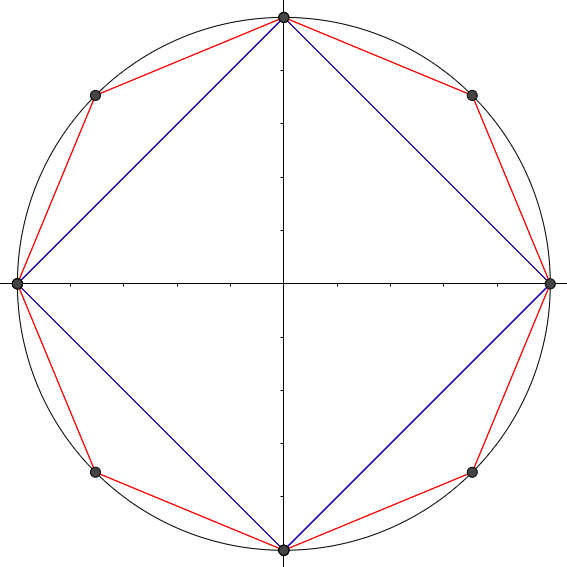
\includegraphics[width=0.5\columnwidth]{img/circlelinear}
    \caption{If the velocity is limited to a finite value, the velocity vector must lie within the circle centered on the origin with the radius equal to that value. This is represented by the black circle. This circle cannot be approximated in MILP, but it can be approximated using several linear constraints. The blue square shows the approximation using 4 linear constraints. The red polygon uses 8 linear constraints. As more constraints are used, the approximation gets closer and closer to the circle. }\label{fig:circlelinear}
\end{figure}
Like any vehicle, a UAV has a certain maximum velocity. The model should contain constraints which prevent the UAV from moving faster than the maximum velocity. The magnitude of the velocity is the 2-norm of the velocity vector (which is Pythagoras' theorem for a 2D vector). This cannot be represented as a linear constraint because the components of the velocity vector need to be squared. However, the 2-norm can be approximated using multiple linear constraints. \\
Figure \ref{fig:circlelinear} visualizes how this works for the 2D case. All velocity vectors with a magnitude smaller than the maximum velocity are on the inside of the black circle with radius $v_{max}$. This cannot be expressed in MILP, but a regular polygon which fits inside the circle can be expressed. As the amount of vertices $N_{vertex}$ making up the polygon increases, the approximation gets more and more accurate. The coordinates of the vertices of the polygon, $q_{x,i}$ and $q_{y,i}$ are defined by Equations \ref{eq:maxvel-theta}-\ref{eq:maxvel-points-y} in counter-clockwise order.

\begin{equation}
\label{eq:maxvel-theta}
\theta = \dfrac{2\pi}{N_{points}}
\end{equation}
\begin{equation}
\label{eq:maxvel-points-x}
q_{x,i}  = v_{max} * cos( \theta i), \quad 0 \leq i < N_{points}
\end{equation}
\begin{equation}
\label{eq:maxvel-points-y}
q_{y,i}  = v_{max} * sin( \theta i), \quad 0 \leq i < N_{points}
\end{equation}
Like before, the equations are limited to the 2D case, but can be extended to 3D as well. Each edge of the polygon defines a line with slope $a_i$ and intercept $b_i$, as determined by Equations \ref{eq:lin-delta}-\ref{eq:lin-b}.

\begin{equation}
\label{eq:lin-delta}
\Delta q_{x,i} = q_{x,i} - q_{x,i-1}, \quad \Delta q_{y,i} = q_{y,i} - q_{y,i-1}
\end{equation}
\begin{equation}
\label{eq:lin-a}
a_i = \dfrac{\Delta q_{y,i}}{\Delta q_{x,i}} \quad 0 \leq i < N_{vertex}
\end{equation}
\begin{equation}
\label{eq:lin-b}
b_i = q_{y,i} - a_i q_{x,i}  \quad 0 \leq i < N_{vertex}
\end{equation}


Finally, the constraints can be constructed using the slope and intercepts of each line segment. For the edges on the "top" half of the polygon, the velocity vector must stay \emph{below} those edges. This is expressed by Equation \ref{eq:vmax-1}. Similarly, for the bottom half, the velocity vector must stay \emph{above} those edges as expressed by Equation \ref{eq:vmax-2}. If $N_{vertex}$ is odd, the left-most edge of the polygon is vertical. Equation \ref{eq:vmax-3} handles this special case: the velocity vector must stay on the right of the left-most edge. TODO: add figure to explain better.

\begin{align}
vy_{n} &\leq a_i vx_{n} + b_i,  & \Delta q_{x,i} < 0, \quad 0 \leq n < N  \label{eq:vmax-1} \\
vy_{n} &\geq a_i vx_{n} + b_i,  & \Delta q_{x,i} > 0, \quad 0 \leq n < N \label{eq:vmax-2} \\
vx_{n} &\geq q_{x,i},  & \Delta q_{x,i} = 0, \quad 0 \leq n < N \label{eq:vmax-3}
\end{align}

The acceleration and other vector properties of the vehicle can be limited in the same way. 
\subsection{Obstacle avoidance}
\label{subsec:obs-avoid}
\begin{figure}[!t]
    \centering
    
    \begin{subfigure}[t]{0.47\textwidth}
        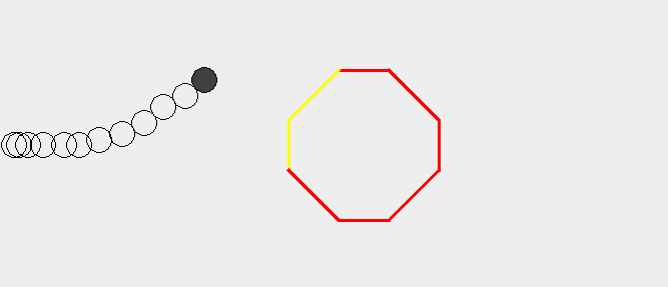
\includegraphics[width=\textwidth]{img/obs1}
        \caption{}
    \end{subfigure}
    \hfil
    \begin{subfigure}[t]{0.47\textwidth}
        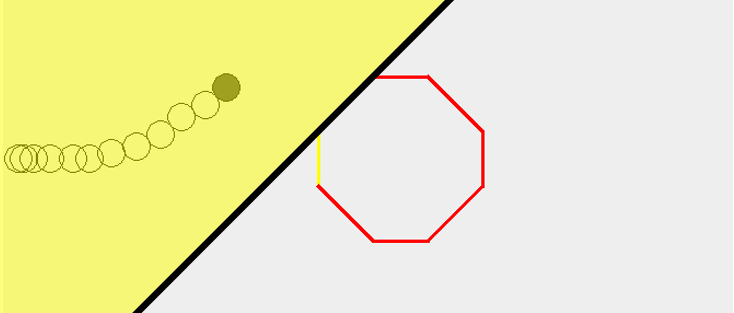
\includegraphics[width=\textwidth]{img/obs2}
        \caption{}
    \end{subfigure}
    \par\bigskip
    \begin{subfigure}[t]{0.47\textwidth}
        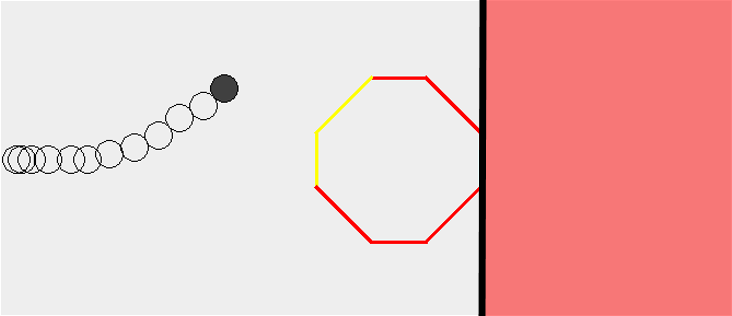
\includegraphics[width=\textwidth]{img/obs3}
        \caption{}
    \end{subfigure}
    \caption{A visual representation of how obstacle avoidance works. The top image shows the vehicle's current position as the filled circle, with its path in previous time steps as hollow circles. The color of the edges of the obstacle represent whether or not the vehicle is in the safe zone for that edge. An edge is yellow if the vehicle is in the safe zone, and red otherwise. The middle image shows the safe zone defined by a yellow edge in yellow. Note how the vehicle is on one side of the black line and the obstacle is entirely on the other side. The bottom image shows an edge for which the vehicle is not in the safe zone (represented in red this time). As long as the vehicle is in the safe zone of at least one edge, it cannot collide with the obstacle.}\label{fig:obs}
\end{figure}
The last element of the model is obstacle avoidance. Obstacles are regions in the world where the UAV is not allowed to be. This may be due to a physical obstacle, but it could also be a no-fly zone determined by law or other concerns. \\
Assuming that each obstacle is a 2D convex polygon, the constraints for obstacle avoidance are similar to those of the vehicle state limits in Section TODO:ref. However, the big difference is that the UAV must stay on the outside of the polygon instead of the inside. \\
\subsubsection{Importance of Convexity}
The maximum velocity is modeled without using any integer variables. This is possible because the allowed region for the velocity vector is a convex shape. A shape is convex if a line drawn between any two points inside that shape is also fully inside the shape. This is demonstrated in Figure \ref{fig:convex-example}\\
This property does not hold for obstacle avoidance. If the UAV is on one side of an obstacle, it cannot move in a straight line to the other side of that obstacle. Because of that obstacle, the shape formed by all the positions where the UAV is allowed to be is no longer convex. This can be seen in Figure \ref{fig:nonconvex-example}. \\
To express non-convex constraints, integer variables are needed. This causes the difference between what can be modeled in Linear Programming versus Mixed-Integer Linear Programming: non-convex constraints can be expressed in MILP, while this is not possible in LP.


\begin{figure}[]
    \centering
    
    \begin{subfigure}[]{0.47\textwidth}
        %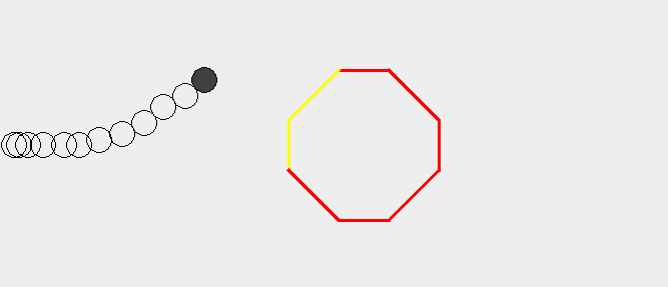
\includegraphics[width=\textwidth]{img/obs1}
        convex
        \caption{TODO:convex}
        \label{fig:convex-example}
    \end{subfigure}
    \hfil
    \begin{subfigure}[]{0.47\textwidth}
        %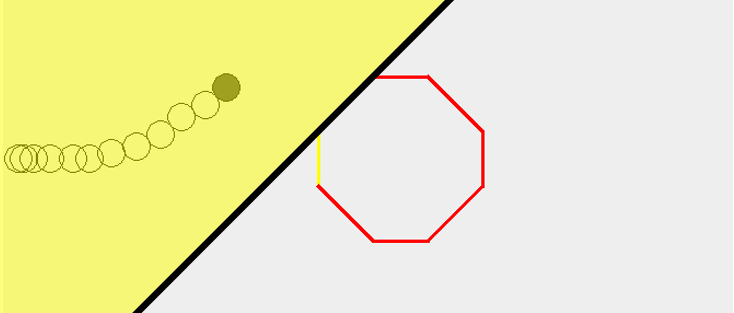
\includegraphics[width=\textwidth]{img/obs2}
        nonconvex
        \caption{TODO:nonconvex}
        \label{fig:nonconvex-example}
    \end{subfigure}
%    \caption{.}\label{fig:obs}
\end{figure}


\subsubsection{Big M Method}
Like with the maximum velocity in Section \ref{subsec:state-limits}, the edges of the obstacle are used to construct the constraints. Each edge defines a line, as determined by Equations \ref{eq:lin-delta}-\ref{eq:lin-b}. If the obstacle is convex, the obstacle will entirely on one side of that line. If the UAV is on the other side, the one without the obstacle, it cannot collide with that obstacle. This region can be consider the safe region defined by that edge. As long as the UAV is in the safe region of at least one edge, no collisions can occur. Figure \ref{fig:obs} demonstrates this visually. \\
A popular way to model this is the "Big M" method TODO:cite. For each edge, a constraint is constructed which forces the UAV to be in the safe region for that edge. However, the UAV must only be in the safe region of at least one edge. This means that it must be possible to "turn off" constraints. \\
For each edge of an obstacle, a boolean $slack$ variable is used to represent whether or the constraint for that edge is enabled. If this $slack$ variable is $true$ (equal to $1$), the constraint is \emph{disabled}. This is where the "Big M" comes in: the $slack$ variable is multiplied by a very large number $M$ on one side of the inequality constraint for that edge. $M$ must be chosen to be large enough to ensure that ,when $slack$ is $true$, the inequality is always satisfied. \\
In Equations \ref{eq:obs-m-1}-\ref{eq:obs-m-4} below, $q_{x,i}$ and $q_{y,i}$ are the 2D coordinates of vertex $i$ the obstacle. The slope $a_{i}$ and intercept $b_{i}$ of edge $i$ are calculated as in Equations \ref{eq:lin-delta}-\ref{eq:lin-b}. For every time step $n$:
\begin{align}
y_{n} \quad + \quad M*slack_{i,n} \quad &\geq 
\quad a_{i} x_{n} + b_{i},  	
& \Delta q_{x,i} < 0 							 	
\label{eq:obs-m-1} \\
y_{n} \quad - \quad M*slack_{i,n} \quad &\leq 
\quad a_{i} x_{n} + b_{i},
& \Delta q_{x,i} > 0 							 	
\label{eq:obs-m-2} \\
x_{n} \quad - \quad M*slack_{i,n} \quad &\leq
\quad  q_{x,i}, 		
& \Delta q_{y,i} < 0, \quad \Delta q_{x,i} = 0 	
\label{eq:obs-m-3} \\
x_{n} \quad + \quad M*slack_{i,n} \quad &\geq 
\quad q_{y,i},  		
& \Delta q_{y,i} > 0, \quad \Delta q_{x,i} = 0 	
\label{eq:obs-m-4}
\end{align}
\begin{figure}
    \centering
        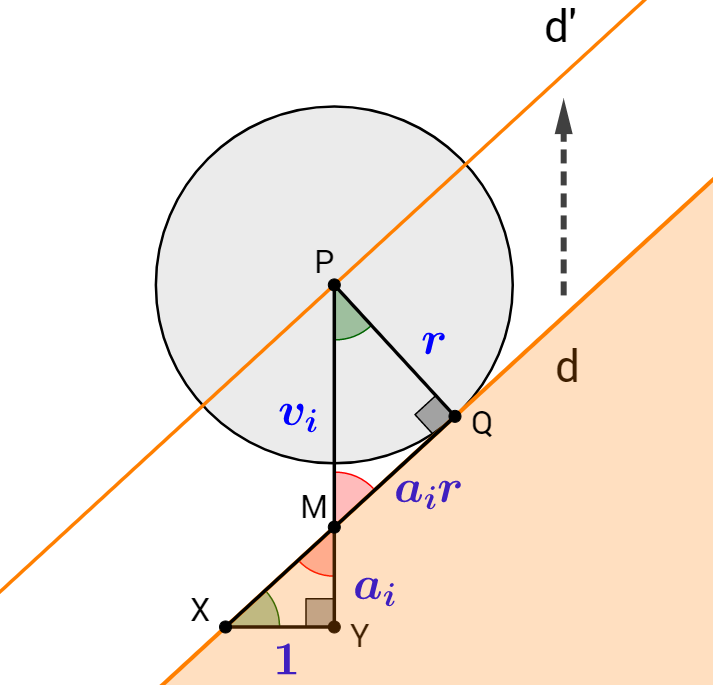
\includegraphics[width=0.8\columnwidth]{offset}
    \caption{A geometric proof for the vehicle offset formula in Equation \ref{eq:offset}. Measures are marked in blue. $P$ is the center of mass of the UAV. $d$ is the line defined by edge $i$ of an obstacle. The obstacle is the orange region. We wish to translate $d$ vertically to $d'$ such that when the UAV's center of mass $P$ touches $d'$, the circle with radius $r$ (representing the UAV's shape, colored in grey) touches $d$ in $Q$. If $d'$ is used for the constraint instead of $d$, the UAV cannot collide with the obstacle. The difference between the intercepts of $d$ and $d'$ is $v_i = |PM|$. The slope of $d'$ is $a_i$, so if $XY$ is horizontal and $|XY| = 1$, then $|MY| = a_i$. Corner $M$ is the same in both triangle $PQM$ and $XYM$, as marked in red. Corner $Q$ and $Y$ are both right angles. This means $PQM$ and $XYM$ are similar triangles. As a result: if $|PQ| = r$, then $|QM| = a_ir$. Using Pythagoras' theorem: $v_i = \sqrt{r^2 + a_i^2r^2} = r\sqrt{1+a_i^2}$.}\label{fig:offset-proof}
\end{figure}
Like in Equations \ref{eq:vmax-1} and \ref{eq:vmax-2}, edges on the top and bottom of the obstacle are treated differently. Equation \ref{eq:obs-m-1} covers the top edges. The UAV must be above the edge. If the UAV is not above the edge (when $y_n$ is too small), enabling $slack_{i,n}$ will add $M$ on the left-hand side of the inequality and ensure that it is always larger than the right-hand side. Equation \ref{eq:obs-m-2} does the same for edges on the bottom. The inequality is flipped around so that the UAV must be below the edge This also means that $M$ must be subtracted from the left-hand side of the inequality to ensure the constraint is always satisfied. \\
Vertical edges are also possible. A vertical edge may occur on the left or right side of the polygon, as covered in Equations \ref{eq:obs-m-3} and \ref{eq:obs-m-4} respectively.\\
Finally Equation \ref{eq:obs-slack} ensures that at least one of the slack variables must be false at each time step.
\begin{equation}
\neg \mathlarger{\mathlarger{\bigwedge_{i}}} slack_{i,n} \quad 0 \leq n \leq N
\label{eq:obs-slack}
\end{equation}

Equations \ref{eq:obs-m-1} - \ref{eq:obs-m-4} assume that the UAV has no physical size. The position of the UAV is the position of its center of mass. Because a UAV has certain physical dimensions, it will collide with an obstacle before its center of mass reaches the obstacle. The vehicle's shape is approximated as a circle with radius $r$. The vertical offset $v_i$ required to move the line with slope $a_i$ from the center of the circle to the edge is calculated by Equation \ref{eq:offset}. A geometric proof is given in Figure \ref{fig:offset-proof}.
\begin{equation}
v_{i} = r \sqrt{1 + a_i^2}
\label{eq:offset}
\end{equation}

With the vertical offset calculated, Equations \ref{eq:obs-m-1} - \ref{eq:obs-m-4} can be extended to Equations \ref{eq:obs-m-1-v}-\ref{eq:obs-m-2-v} which take the UAV size into account.

\begin{align}
y_{n} + M*slack_{i,n} \quad &- \quad v_i \quad \geq 
\quad a_{i} x_{n} + b_{i},  	
& \Delta q_{x,i} < 0 							 	
\label{eq:obs-m-1-v} \\
y_{n} - M*slack_{i,n} \quad &+ \quad v_i \quad \leq 
\quad a_{i} x_{n} + b_{i},
& \Delta q_{x,i} > 0 							 	
\label{eq:obs-m-2-v} \\
x_{n} - M*slack_{i,n} \quad &+ \quad r \quad \leq
\quad  q_{x,i}, 		
& \Delta q_{y,i} < 0, \quad \Delta q_{x,i} = 0 	
\label{eq:obs-m-3-v} \\
x_{n} + M*slack_{i,n} \quad &- \quad r \quad \geq 
\quad q_{y,i},  		
& \Delta q_{y,i} > 0, \quad \Delta q_{x,i} = 0 	
\label{eq:obs-m-4-v}
\end{align}


%\begin{figure}
%	\centering
%	\begin{subfigure}[t]{1\columnwidth}
%        		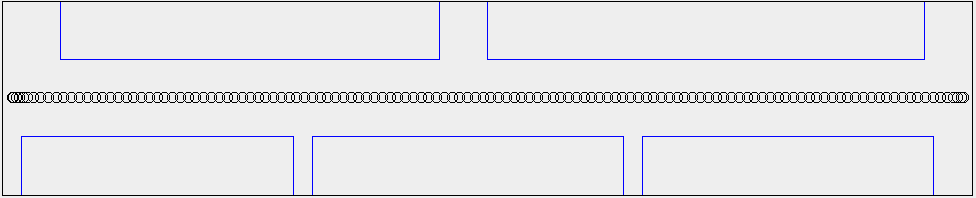
\includegraphics[width=\textwidth]{small-bench-flat}
%        		\caption{The horizontal scenario.}
%        		\label{fig:convex-straight}
%	\end{subfigure}
%	\par\bigskip
%	\begin{subfigure}[t]{1\columnwidth}
%        		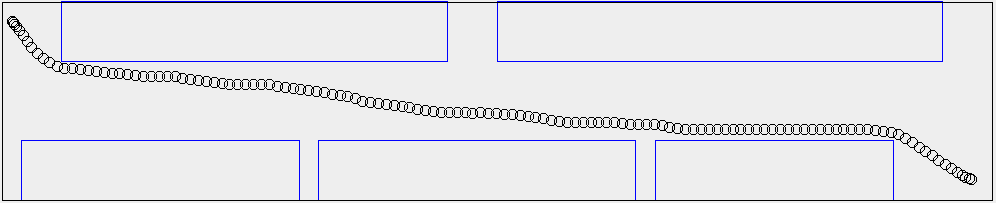
\includegraphics[width=\textwidth]{small-bench-diag}
%        		\caption{The diagonal scenario.}
%        		 \label{fig:convex-diag}
%	\end{subfigure}	
%	\par\bigskip
%	\begin{subfigure}[t]{0.8\columnwidth}
%        		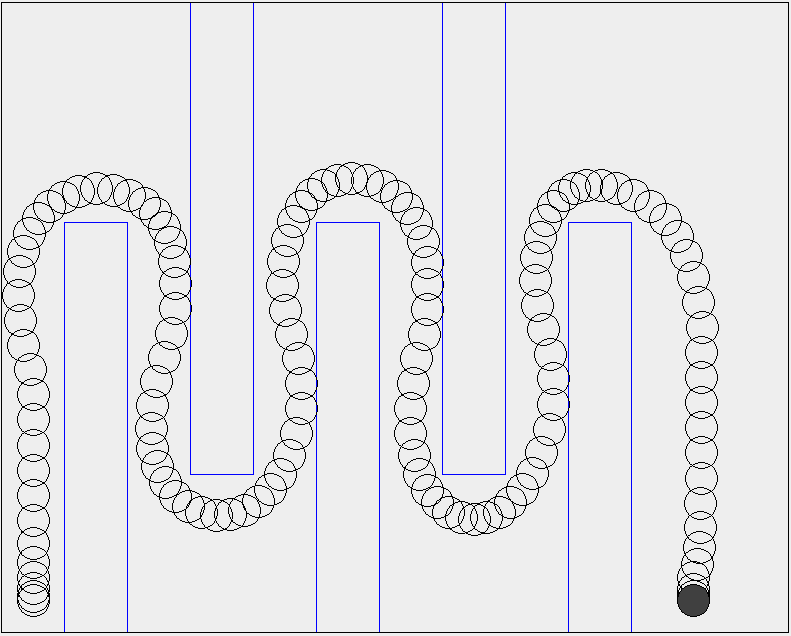
\includegraphics[width=\textwidth]{small-bench}
%        		\caption{The Up/Down Scenario.}
%        		 \label{fig:convex-full}
%	\end{subfigure}	
%    \caption{Three different testing scenarios, each with the same amount of obstacles. In each scenario, the UAV needs nearly the same amount of time steps to reach its goal. The only difference is the layout of the obstacles.}
%    \label{fig:benchmarks}     
%\end{figure}
%\clearpage
%\subsection{Performance}
%
%\begin{figure}[]
%	\centering
%	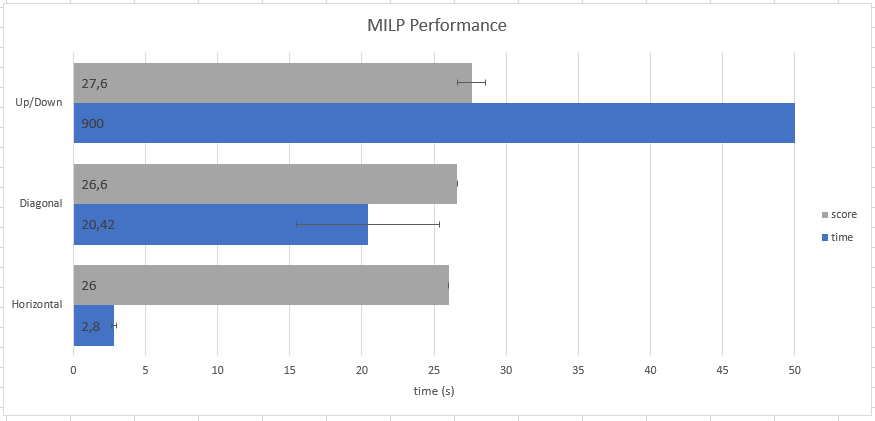
\includegraphics[width=\textwidth]{naive-performance}
%	\caption{Performance of the MILP problem.}
%	\label{fig:naive-performance}
%\end{figure}
%Typically, the amount of integer variables is used as a metric for the difficulty of a MILP problem. The amount of integer variables determines the worst case time needed to solve the MILP problem. An integer variable is needed for every edge, for every obstacle, for every time step. Increasing the amount of time steps and obstacles also increases the time needed to solve.\\
%However, the amount of integer variables does not seem to be the only factor that determines the solve time. Figure \ref{fig:benchmarks} shows three different scenarios, each with the same amount of obstacles. The time step size is $0.2s$, and in each scenario there were 30 seconds worth of time steps. The scenarios are built such that the time needed for the UAV to reach the goal position is roughly the same (between 26 and 27 seconds). As a result, each scenario has the same amount of integer variables. With 4 edges for all 5 obstacles and 150 time steps, they each have 3000 integer variables to model the obstacles alone.\\
%
%In the Horizontal scenario, the obstacles are not in the way of the UAV. The UAV can move in a straight line from the start position to its goal. In the Diagonal scenario, two of the obstacles are slightly in the way. The UAV is forced to make slight turns near the start and end of the trajectory. However, most of the trajectory is still straight. In the Up/Down scenario, the vehicle has to slalom around every obstacle.\\
%The convexity of the search space plays a large role in the difficulty of a MILP problem. My approach is built entirely around the idea of keeping the search space as convex as possible in each segment. To analyze  the importance of convexity, I tested three scenarios without any form of preprocessing. These scenarios are designed so the optimal trajectory has roughly the same duration in each scenario. The scenarios also each have 5 grid aligned rectangles as obstacles.\\
%As a result, MILP problems for all three scenarios have nearly identical amounts of integer variables. The difference between these scenarios is the convexity of the search space. \\


%\subsubsection{Results}
%Each scenario was solved five times. Figure \ref{fig:naive-performance} shows the time needed to solve the models, as well as the score. The score is also expressed in seconds, and is the time needed for the UAV to reach the goal position when following the generated trajectory. \\
%The time needed to solve these scenarios varies dramatically. The Horizontal scenario is solved consistently in just under 3 seconds. The Diagonal scenario comes in at around 20 seconds, although the 95\% confidence interval is $\pm 4.9s$. The Up/Down scenario was limited to 900s of execution time. In this time, the solver could not find the optimal trajectory, which is why the score has a confidence interval.
%\subsubsection{Discussion}
%Intuitively, it is not surprising that the Up/Down scenario is harder to solve than the other two. A human pilot would also have more difficulties navigating the Up/Down scenario compared to the others. However, this is cannot be determined by looking a the amount of integer variables or constraints alone.\\
%Problems where the trajectory requires maneuvers seem to be harder to solve. The maneuvers are necessary because there are obstacles blocking a straight approach to the goal position. This observation led me to believe that the integer variables themselves do not cause the poor performance, but the real issue is what they model: a non-convex search space.\\
%The amount of integer variables determines the worst-case performance because it determines the degree to which the search space can be non-convex. An informal definition of this degree of non-convexity would be the minimum amount of (possibly overlapping) convex shapes needed to reconstruct the original shape. With a single boolean variable, you need at most 2 convex shapes. With $n$ boolean variables, at most $2^n$ convex shapes are needed. TODO: cite.\\
%\begin{figure}
%	\centering
%	\begin{subfigure}[t]{0.47\columnwidth}
%        		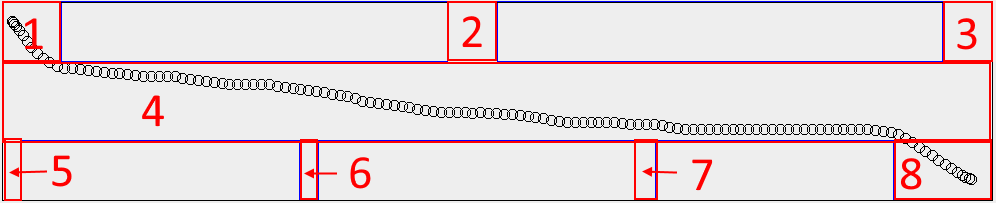
\includegraphics[width=\textwidth]{small-bench-diag-convexity}
%        		\caption{8 convex regions are needed to reconstruct the diagonal scenario.}
%        		 \label{fig:convex-diag-convexity}
%	\end{subfigure}	
%	\hfill
%	\begin{subfigure}[t]{0.47\columnwidth}
%        		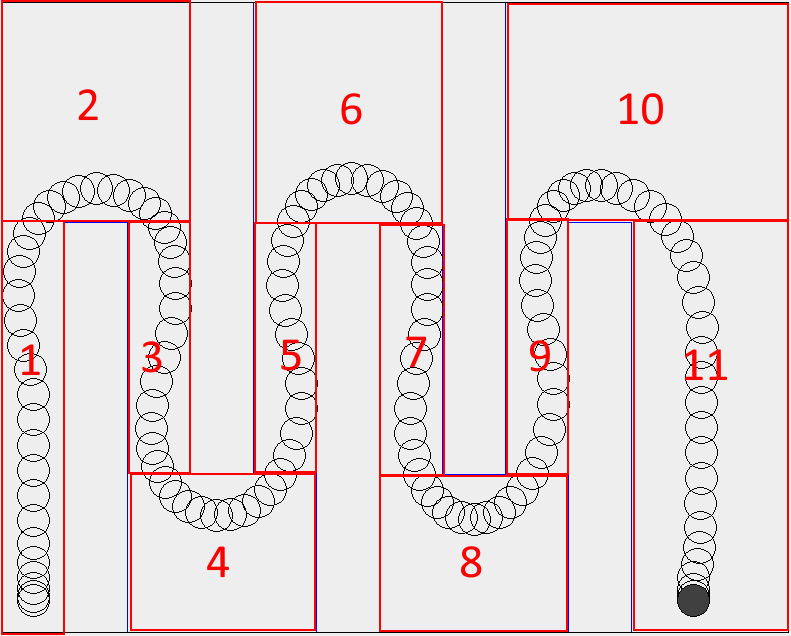
\includegraphics[width=\textwidth]{small-bench-convexity}
%        		\caption{11 convex regions needed to reconstruct the Up/Down Scenario.}
%        		 \label{fig:convex-full-convexity}
%	\end{subfigure}	
%    \caption{}
%    \label{fig:benchmarks-convex}     
%\end{figure}
%The degree of convexity of the open space for the Up/Down scenario is 11 as shown in Figure \ref{fig:convex-full-convexity}. For the Horizontal and Diagonal scenarios, this is 8 as shown in Figure \ref{fig:convex-diag-convexity}. There is a difference, but this still does not seem like a good explanation. The Horizontal and Diagonal scenarios have the same degree of convexity, even though there's almost an order of magnitude difference in the solve times. \\
%Even though the global degree of convexity is the same for the Horizontal and Diagonal scenarios, this is not the case for the neighborhood around the trajectory. In the Horizontal scenario, the trajectory only goes through a single convex region. In the Diagonal scenario, the trajectory goes through 3 convex regions. For the Up/Down scenario, the trajectory goes through all 11 regions. I present the following hypothesis:
%\begin{hyp}
%The degree of non-convexity around the optimal trajectory is a better indicator of the time needed to solve a MILP trajectory planning problem than the amount of integer variables.
%\label{hyp:nonconvex}
%\end{hyp}
%
%\subsubsection{Implications for the thesis}
%While I present Hyptothesis \ref{hyp:nonconvex} before my algorithm, I actually only came up with it near the end of the project when the algorithm was already completed. The development of the algorithm was based on a lot of trial and error, exploiting the ideas that work and ignoring those that do not. MILP solvers are black boxes, so it is hard to predict which ideas will work and which do not. It is not uncommon for mathematically equivalent constraints to have drastically different effects on solve time. \\
%However, near the end of the project I started to understand the behavior of the solver better. Hypothesis \ref{hyp:nonconvex} is the result of what I have learned during the project. It is what I believe to be the core reason why my algorithm is effective.
%\par
%The decisions I made during the development of the algorithm



%%Thoroughly analyzing this hypothesis is outside the scope for this thesis. The goal of this these is to build a scalable MILP trajectory planning algorithm. Many decisions in this thesis assume that this hypothesis is true, even though I cannot provide a more thorough analysis than the arguments presented here.



%However, the degree of non-convexity of a problem may be lower than that upper limit determined by the amount of integer variables.I propose the following hypothesis:\\
%\\
%
%
%
%
%This poor performance scaling is the problem the rest of this thesis attempts to resolve. As the number of integer variables increases, the worst case time needed by the solver increases exponentially.\\
%As a result, solving long trajectories with many obstacles is infeasible with MILP. However, it may be possible to achieve acceptable levels of performance if the MILP problem can be divided into many, smaller sub-problems. Each sub-problem only solves a small part of the trajectory, making it much faster to solve.\\
%To improve the solve time for each sub-problem, the amount of integer variables should be limited. However, I suspect this is short-sighted. Integer variables are a tool which make it possible to express a non-convex search space. \\

%
%number of edges * number of time steps, divide problem in smaller segments and solve one by one: each segment. makes it much faster.
%
%worst case performance is dependent on amount of integer variables. hypothesis: actual performance depends heavily on convexity, not integer variables. Instead of trying to minimize integer variables directly, focus should be on abstraction layer above that by trying to keep convexity as high as possible. This concept is the main assumption going forward.


%\subsection{Importance of integers and convexity}
%TODO: REWRITE
%linear programming one of the most simple forms of mathematical programming. Only linear functions allowed, all variables have a real domain. If feasible region exists: inherently convex. When a problem is convex, typically efficient solvers can be written (TODO: find source). This is the case for LP. LP problems can be solved reliably and quickly.
%\\
%Problem: only real variables is very limiting. Logical operators are impossible to model. Result is that not every problem can be modeled without integers. Adding integers seems like a minor change, but it no longer guarantees that the feasible region is convex. When the problem is no longer convex, it becomes intractible. An intractible problem is a problem for which we do not have a strategy that will on average find the solution faster than random guessing.
%\\
%Path planning when obstacles are present inherently needs integer variables and thus is an intractible problem. The goal of this thesis is to make this approach to path planning scalable. This will rely on two concepts://
%- The solvers are on average not faster than random, but that's the average of all problems. We are only concerned with a very specific kind of problem. By being aware of how the solver works and simply experimenting with different representations, the problem can be solved much faster\\
%- We can cheat. The problem can be greatly simplified and approximated. This means that the solution is no longer guaranteed to be optimal, but as long as it is good enough this is not a problem.\\
%
%\subsection{Characteristics of the basic model}
%Nothing new in basic model, motivate changes based on flaws in the model. demonstration with simple scenario (benchmark and spiral) where basic model already struggles. Approximate amount of integer variables needed, use as representation of nonconvexity of problem. \\
%Also show issue with time allowed: Need to allocate way more time than is needed, making the problem even harder to solve. Limiting time makes problem faster to solve, but cannot know without prior information.\\
%Demonstrate issue with corners. Corners make execution time go up even as amount of integer variables stays the same. If no corners are needed, feasible space stays more convex even though integer values are same. Nuance that integer variables are only apprixmation of non-convexity, convexity is real property that matters.\\
%Conclude: need to reduce amount of obstacles, need to reduce timesteps, limit amount of corners at a time (so problem becomes more convex). Dividing problem into smaller pieces tackles all these goals.

\clearpage
\chapter{Segmentation of the MILP problem}
\label{section:segment}

\section{Scalability of the pure MILP approach}
The MILP model described in chapter \ref{section:modelingbasic} is sufficient to solve the trajectory planning problem for short flights with few obstacles. However, this "pure MILP" approach scales poorly when the amount of time steps or obstacles in the model is increased. The following small experiment demonstrates this.
\par
\begin{figure}[b]
	\centering
	\begin{subfigure}[t]{0.3\columnwidth}
        		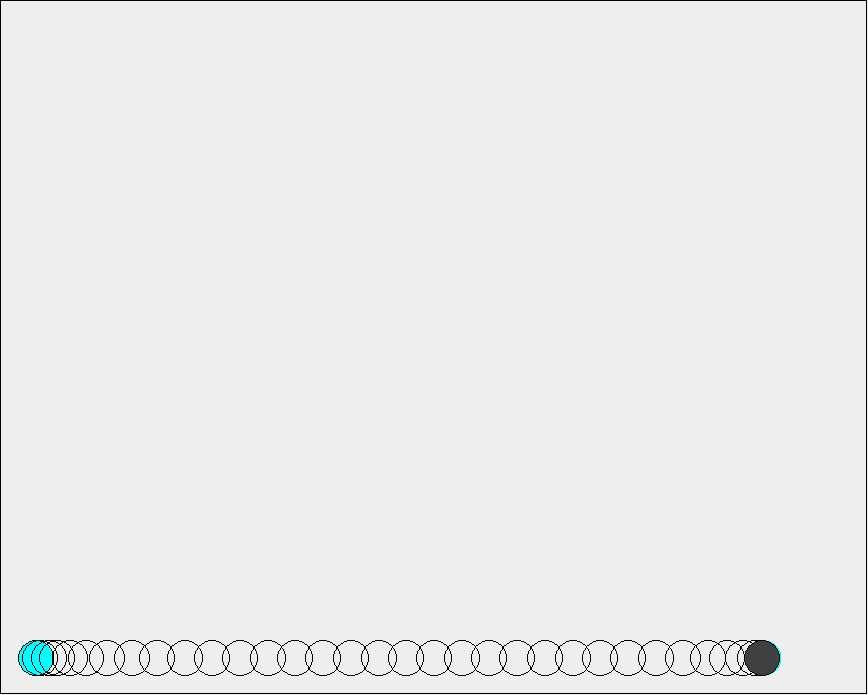
\includegraphics[width=\textwidth]{bench-0}
        		\caption{Up/Down 0}
        		 \label{fig:bench-0}
	\end{subfigure}	
	\hfill
	\begin{subfigure}[t]{0.3\columnwidth}
        		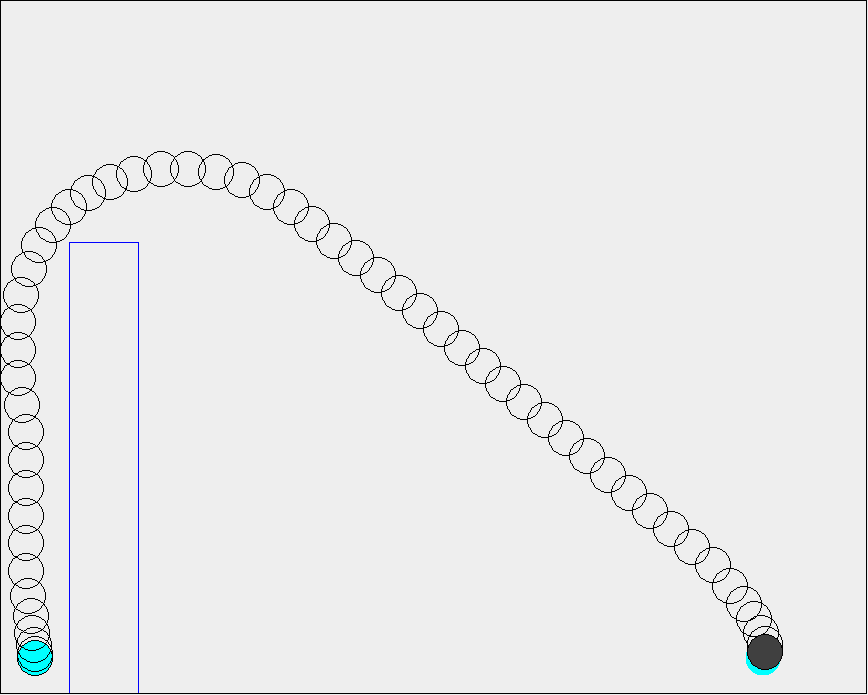
\includegraphics[width=\textwidth]{bench-1}
        		\caption{Up/Down 1}
        		 \label{fig:bench-1}
	\end{subfigure}	
	\hfill
	\begin{subfigure}[t]{0.3\columnwidth}
        		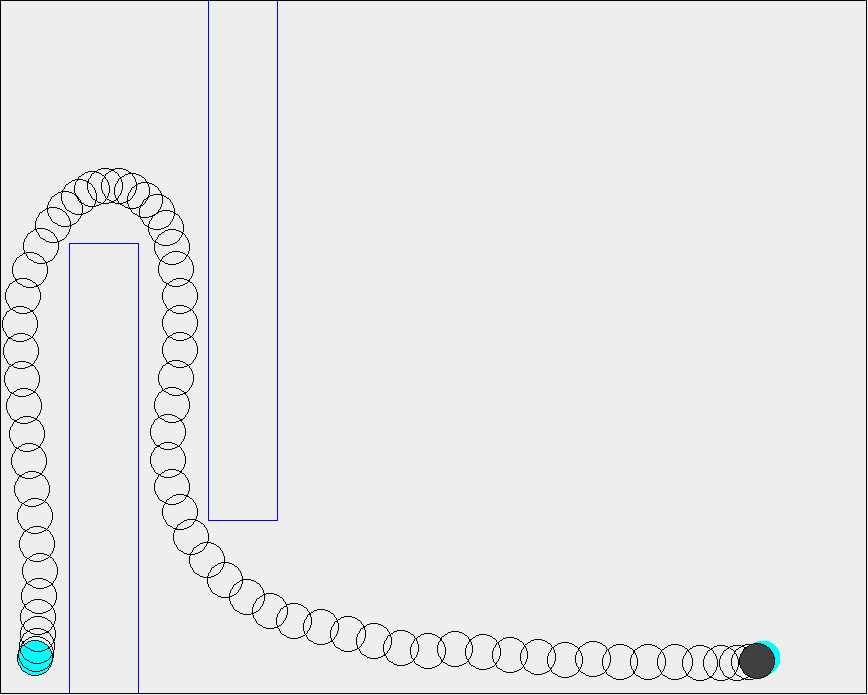
\includegraphics[width=\textwidth]{bench-2}
        		\caption{Up/Down 2}
        		 \label{fig:bench-2}
	\end{subfigure}
%	\par\bigskip
	\begin{subfigure}[t]{0.3\columnwidth}
        		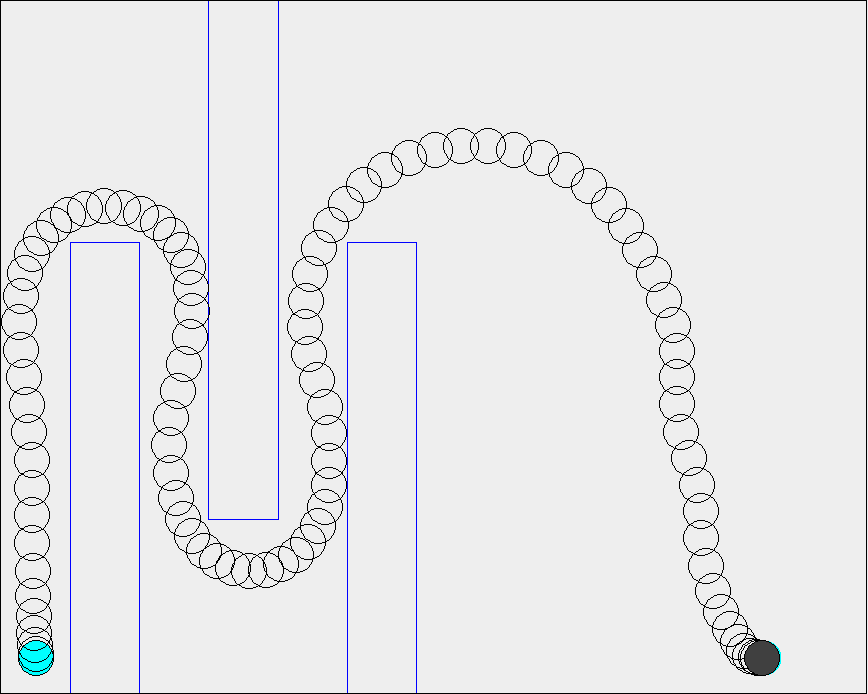
\includegraphics[width=\textwidth]{bench-3}
        		\caption{Up/Down 3}
        		 \label{fig:bench-3}
	\end{subfigure}	
	\hfill
	\begin{subfigure}[t]{0.3\columnwidth}
        		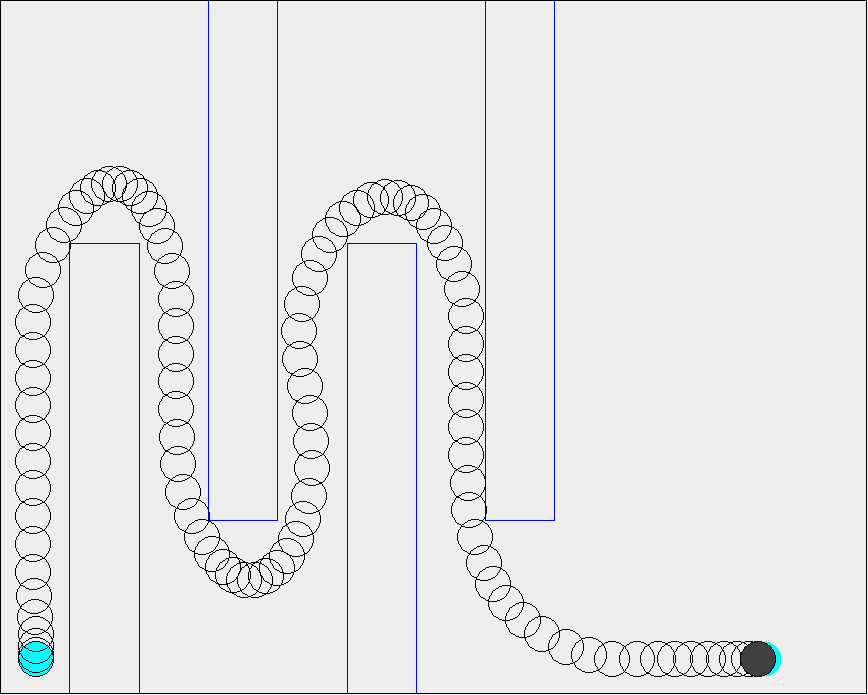
\includegraphics[width=\textwidth]{bench-4}
        		\caption{Up/Down 4}
        		 \label{fig:bench-4}
	\end{subfigure}	
	\hfill
	\begin{subfigure}[t]{0.32\columnwidth}
        		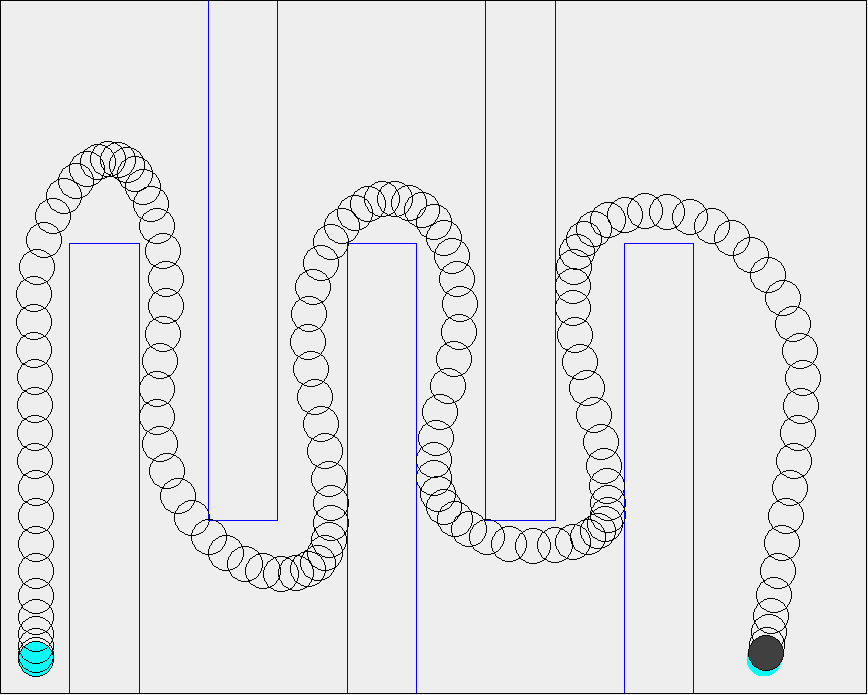
\includegraphics[width=\textwidth]{bench-5}
        		\caption{Up/Down 5}
        		 \label{fig:bench-5}
	\end{subfigure}		
	
			
	\caption[The six variations of the Up/Down scenario]{The six variations of the Up/Down scenario, ranging from no obstacles in \ref{fig:bench-0} to five obstacle in \ref{fig:bench-5}.}
    \label{fig:bench-pure}     
\end{figure}
In the experiment, the UAV must move from a point in the bottom-left corner of the world to a point in the bottom-right corner. Six different scenarios are tested. The different scenarios have a varying amount of rectangular obstacles in their world, ranging from zero at all to five obstacles. These obstacles are laid out in such a way that the UAV must zig-zag up and down to reach its goal. The time step size is $0.2s$, and there are 30 seconds worth of time steps modeled in scenario. 
\par
Figure \ref{fig:bench-pure} shows the different scenarios and the trajectory found as the solution for that scenario. Figure \ref{fig:pure-data} shows a graph of the trajectory scores, measured in seconds. The trajectory score is the time it takes for the UAV to reach its goal when it follows that trajectory. It also shows the execution time. Each scenario was executed 5 times, and execution time was limited to 900 seconds.

\begin{figure}[t]
	\centering
	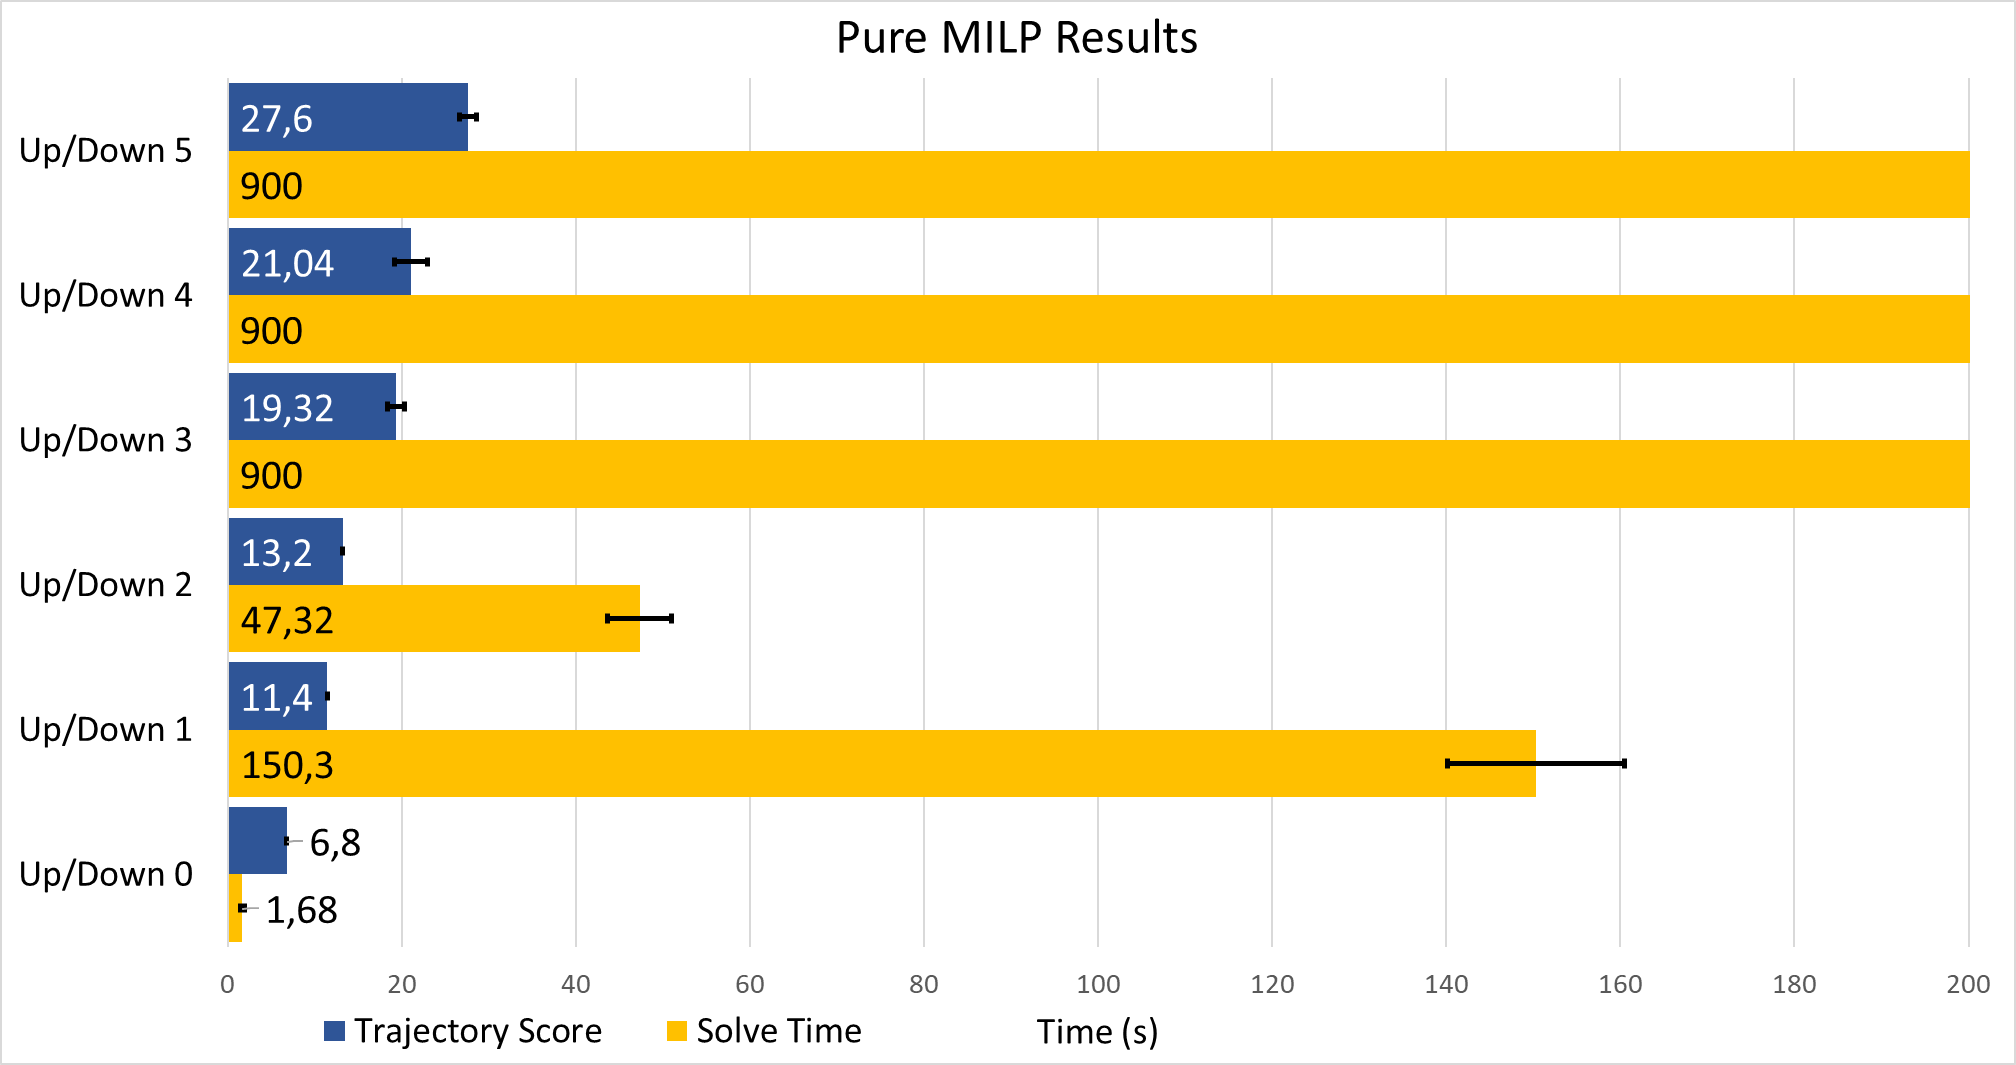
\includegraphics[width=\textwidth]{pure-milp-data}
	\caption[The results for the pure MILP approach ]{The results of the Up/Down scenario for the pure MILP approach with varying numbers of obstacles. The error bars show the 95\% confidence interval.}
	\label{fig:pure-data}
\end{figure}

Without any obstacles, the solver finds the trajectory in under two seconds. However, when even a single obstacle is added, the solver needs more than two minutes to find the optimal trajectory. When another obstacle is added, the solve time drops to below a minute again even though there are more integer variables used in the model. Starting at three obstacles and more, the solver can no longer find the optimal trajectory in less than 15 minutes. Clearly, this is not going to scale well to large scenarios.
\section{Algorithm approach}
Mixed-Integer programming belongs to the ``NP-Complete'' class of problems \cite{DBLP:conf/coco/Karp72}. Assuming there are $n$ boolean variables, the worst case time complexity is $O(2^n)$. A boolean variable is needed for every edge of every polygon, for every time step. By reducing both the amount of time steps needed and the amount of obstacles that need to be modeled, the solve time can be reduced dramatically. \\
The key insight that allows my algorithm to scale well beyond what's usually possible is that the trajectory planning problem does not need to be solved all at once. If the trajectory planning problem can be split into many different subproblems, each subproblem becomes easier to solve. The solution for each subproblem is a small part of the final trajectory. By solving these subproblems sequentially, the final trajectory can gradually be constructed. \\
While splitting the problem into subproblems does make each subproblem much easier to solve, it also has an important down side: finding the fastest trajectory can no longer be guaranteed. Smaller subproblems make it easier to find a solution, but fundamentally the problem of finding the optimal trajectory is still just as hard. The necessary trade-off for better performance is that the optimal trajectory will likely not be found. Luckily, the optimal trajectory is often not required in navigation. A reasonably good trajectory will do.

\subsection{Importance of convexity}
The worst case time needed to solve a MILP problem increases exponentially with the amount of integer variables. However, this is not the most useful way to measure the difficulty of a problem. Modern solvers are heavily optimized and are able to solve certain problems with many integer variables much faster than others. The key difference is the convexity of the solution space. Just like a circle is the solution space for ``all points a certain distance away from the center point'', the constraints used to model the trajectory planning problem form some geometric shape with a dimension for every variable. \\
When only linear constraints with real values are allowed, the solution space will always be convex. It is this convexity that makes a standard linear program easy to solve. When integer variables are introduced, it is possible to construct solution spaces which are not convex. As the solution space becomes less and less convex, the problem becomes harder to solve. Integer variables can be seen as a tool which allows non-convex solution spaces to be modeled. When trying to improve the difficulty of a problem, the actual goal is making the problem more convex (or smaller, which always helps). Reducing the amount of integer variables is only a side effect. \\
This insight is critical when determining how to divide the trajectory problem into smaller subproblems, and which obstacles are important for each subproblem.
\newpage
\begin{algorithm}[t]
\caption{General outline}
\label{alg:outline}
\begin{algorithmic}[1]
\State $T \leftarrow \{\}$ \Comment{The list of solved subtrajectories}
\State $path \leftarrow$ \Call{Theta*}{$scenario$}
\State $events \leftarrow$ \Call{FindTurnEvents}{$path$}
\State $segments \leftarrow$ \Call{GenSegments}{$path$, $events$}
\ForEach {$segment \in segments$}
\State \Call{UpdateStartState}{$segment$}
\State \Call{GenSafeRegion}{$scenario$, $segment$}
\State \Call{GenSubMILP}{$scenario$, $segment$}
\State $T \leftarrow T \cup \{$ \Call{SolveSubMILP}{} $\}$
\EndFor
\State $result \leftarrow $\Call{MergeTrajectories}{$T$}
\end{algorithmic}
\end{algorithm}

\subsection{General Algorithm Outline}
Algorithm \ref{alg:outline} shows the general outline of the algorithm. It consists of two phases. The first phase gathers information about the trajectory planning problem. A Theta* path planning algorithm is used to find an initial path (line 2). Unlike a trajectory, a path is time-independent and does not take the UAV's dynamics into account. From this initial path, turn events are generated (line 3). These turn events mark where the trajectory will have to turn. \\
The second phase builds and solves "segments". Each segment represents a single sub-trajectory. The segments contain the information needed to build the corresponding MILP subproblem, which can in turn be solved by the solver to find the sub-trajectory. First, each segment is generated (line 3) from the turn events found in the previous step. Before the MILP sub-problem can be generated and solved (line 8-9), a heuristic selects several obstacles to be modeled in the problem. A genetic algorithm generates a safe region which is allowed to overlap those selected obstacles only (line 7). To ensure a seamless transition between two consecutive sub-trajectories, the starting state for the UAV in the MILP problem for the current segment is updated to match the final state of the UAV in the previous segment (line 6). Finally, the sub-trajectories are merged together to form the final trajectory (line 11).

\section{Finding the initial path}
\label{subsec:initial-path}
The first step in Algorithm \ref{alg:outline} is finding the Theta* path (line 2). This path will be used to split the trajectory planning problem into segments. The MILP problem generated from each of those segments needs an intermediate goal to get the UAV closer to the final goal position. These intermediate goals will be determined by the Theta* path. \\
This path is not only useful to guide the trajectory towards the goal. It also lets the algorithm determine where the turns will be in the trajectory, since the turns in the trajectory will match the turns in the Theta* path.

\subsection{A*}
Theta* is a variant of the A* path planning algorithm. In A*, the world is represented as a graph. Each possible position is represented as a node in that graph, with edges between nodes if one position can be reached from the other. The distance between connected positions is represented as a weight or cost on each edge. \\
Planning a path consists of picking a start and goal node. The A* algorithm will traverse the edges between nodes, keeping track of which edges it traversed to reach a certain node. When the algorithm reaches the goal node, the nodes visited to reach that goal node are the path from the start node to the goal . \\
In this thesis, the world the UAV travels through is a continuous (2D) world. The graph for A* is generated by overlaying a grid on the world. Nodes are placed at each intersection of the grid, as long as they are not inside obstacles. Each node is also connected to its neighbors by moving horizontally, vertically or diagonally along the grid. Figure \ref{fig:astar-grid} shows an example of this.
\begin{figure}
\centering
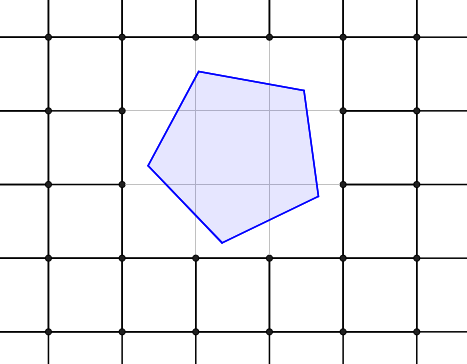
\includegraphics[width=0.5\textwidth]{astar-grid}
\caption[The grid used to build the graph for the Theta* algorithm]{An example of how a grid is used to build the graph for the path finding algorithm. Each point is a node on the graph. If two points are connected by a line, their nodes in the graph also are connected by an edge. Diagonal edges are not shown here for clarity.}
\label{fig:astar-grid}
\end{figure}

\begin{figure}[h]
\centering
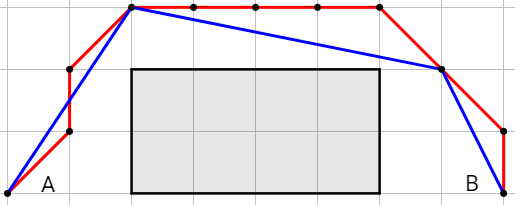
\includegraphics[width=0.5\textwidth]{a_theta_star_comp3}
\caption[A comparison between an A* and Theta* path]{The red line shows a typical A* path, compared to the path found by Theta*. The gray rectangle is an obstacle.}
\label{fig:thetastarcompare}
\end{figure}

\subsection{Reason for Theta*}
A* finds the shortest path through the graph. However, this graph is only an approximate representation of the actual continuous world. An A* path will only travel along the edges of the graph. This means that the path can only travel horizontally, vertically and possibly diagonally. If the shortest path between two points is at another angle, the A* path will contain zig-zags or detours because it is limited to traveling along the grid. \\
Theta* solves this problem. It is nearly identical to A*, but it allows the path to travel at arbitrary angles. It still traverses the graph using the edges between nodes, but does not restrict the path to only following those edges. Figure \ref{fig:thetastarcompare} shows the effect of this change.




\subsection{Theta* implementation}

Theta* was originally developed by Daniel et al. \cite{Daniel2010}. This section, including Algorithm \ref{alg:thetastar}, paraphrases their excellent explanation of the algorithm. The implementation is shown in Algorithm \ref{alg:thetastar}, which uses the following elements:
\begin{itemize}
\item The g-value $g(s)$ is the length of the shortest path between the start node and $s$.
\item A function $c(s,s')$ which returns the distance between node $s$ and $s'$.
\item A heuristic function $h(s)$, which approximates the path distance left before the goal position $s_{goal}$ is reached. The straight line distance between $s$ and the $s_{goal}$ is used, such that $h(s) = c(s,s_{goal})$. An admissible heuristic function must always be an underestimation of the actual path distance to the goal, which is ensured by using the straight line distance. 
\item A function $parent(s)$ which returns the node before $s$ in the path. When the parent of a node is $null$, it is either not part of the path or the first node of the path.
\item A priority queue $queue$. This is a queue of nodes to expand next. Each node $s$ is added with a value $x$ using the $queue.$Insert($s$,$x$) method. If $s$ is already in $queue$, its value is updated to $x$. The $queue$.Pop() method removes and returns the node $s$ with the lowest value $x$.
\item A set $expanded$ which contains all nodes which have already been expanded.
\item A function GenerateNeighbors($s$) which generates and returns the neighbors of node $s$. These are the neighboring positions on the grid around $s$
\end{itemize}

\begin{algorithm}[h]
\caption{Theta* Implementation}
\label{alg:thetastar}
\begin{algorithmic}[1]
\Function{Theta*}{$scenario$}
	\State $g(v_{start}) \leftarrow 0$
	\State $parent(v_{start}) \leftarrow null$
	\State $queue \leftarrow \emptyset$
	\State $queue$.Insert($v_{start}$, $g(v_{start}) + h(v_{start})$)
	\State $expanded \leftarrow \emptyset$
	\While{$queue \neq \emptyset$}
		\State $s \leftarrow queue$.Pop()
		\If{$s = v_{goal}$}
			\Return $s$.GetPath()
		\EndIf
		\State $expanded \leftarrow expanded \cup \{s\}$
		\ForEach{$s' \in ~ $GenerateNeighbors($s$)}
			\If{$s' \notin expanded $}
%				\If{$s' \notin queue$}
%					\State{$g(s') \leftarrow \infty $}
%					\State{$parent(s') \leftarrow null $}
%				\EndIf
				\State{UpdateVertex($s$,$s'$)}
			\EndIf
		\EndFor
	\EndWhile
	\Return "no path found"
\EndFunction
\Function{UpdateVertex}{$s$,$s'$}
	\If{LineOfSight($parent(s)$,$s'$)}
		\State $s_{parent} \leftarrow parent(s)$
	\Else
		\State $s_{parent} \leftarrow s$	
	\EndIf
	\If{$g(s_{prev}) + c(s_{prev},s') < g(s')$}
		\State $g(s') \leftarrow g(s_{parent}) + c(s_{parent},s')$
		\State $parent(s') \leftarrow s_{parent}$
		\State $queue$.Insert($s'$,$g(s') + h(s')$)
	\EndIf
\EndFunction{}
\end{algorithmic}
\end{algorithm}
\paragraph{Initialization}
When the algorithm initializes, the g-value of the start node $v_{start}$ is set to zero and its parent is set to $null$ (line 2-3). The priority queue $queue$ is initialized, and $v_{start}$ is added to it with value $g(v_{start}) + h(v_{start})$. The value attached to a node $v$ in the priority queue is the shortest possible length of a path going from the start $v_{start}$ to the goal $v_{goal}$, while going through $v$. The g-value is the length of the path between $v_{start}$ and $v$, while $h(s)$ is an estimate of the length of the path between $v$ and $v_{goal}$.
\paragraph{Main loop}
$queue$.Pop() always removes the node $s$ with the lowest value (line 8). This means that as more nodes get added to $queue$, the algorithm will always explore the "most promising leads" first. If $s = v_{goal}$, the goal has been reached and the path is returned (line 9-11). Otherwise, $s$ is added to $expanded$ (line 12). This prevents $s$ from being added to $queue$ again. Line 13 generates every neighbor $s'$ of $s$ according to the grid and obstacles, as seen in Figure \ref{fig:astar-grid}, "expanding" node $s$. If the neighbor $s'$ has not been expanded yet, UpdateVertex($s$,$s'$) is called (line 14-16).
\paragraph{UpdateVertex}
So far, the algorithm is identical to A*. The only difference between A* and Theta* are lines 22-26. Line 22 checks if the parent of $s$, which is the node before $s$ in the path, can be connected in a straight line to $s'$. Going from $parent(s)$ to $s'$ directly is always shorter than going from $parent(s)$ to $s$ and from $s$ to $s'$ due to the triangle inequality. If $parent(s)$ and $s'$ are in line of sight, the path should be constructed from $parent(s)$ to $s'$, skipping $s$. Otherwise, the path goes through $s$, which is the behavior  of A*. The choice of which node should be the parent of $s'$ is stored as $s_{parent}$\\
Line 27 checks if the path through $s_{parent}$ to $s'$ is the shortest path to $s'$ found so far. If this is not the case, a shorter path to $s'$ exists so the  path through $s_{parent}$ can safely be ignored. Otherwise, the g-value of $s'$ is updated to the length of the path to $s_{parent}$, $g(s_{parent})$ plus the distance between $s_{parent}$ and $s'$, $c(s_{parent},s')$ (line 28). The shortest path to $s'$ is updated by setting $parent(s')$ to $s_{parent}$ (line 29). Finally, $s'$ is added to $queue$ to be expanded further.
\subsection{Performance improvements}
By introducing the line of sight check, Theta* is considerably slower than A* in large worlds with many obstacles. The goal of this thesis is to improve scalability of trajectory planning to large and complex worlds, so the preprocessing phase must also scale well. \\
To help Theta* scale better, the world is divided into rectangular sectors. When the world is first loaded, the algorithm determines in which sector(s) each obstacle is placed, creating an index mapping sectors to obstacles. \\
When the line of sight check is executed, the algorithm determines which sectors the line crosses. This is usually just one or two sectors. By using the index, only the obstacles in those sectors need to be considered for the line of sight check. This is much faster than having to check every obstacle in the entire world every time.



\section{Detecting turn events}
\label{subsec:corner-events}
%According to Hypothesis \ref{hyp:nonconvex}, the degree of non-convexity around the trajectory is responsible for the poor performance of MILP trajectory planning problem. This local degree of non-convexity around the trajectory is the amount of distinct convex shapes the trajectory needs to pass through to reach the goal position, such that every point in the trajectory lies within at least one shape. \\
%Within a single convex shape, by definition, it is always possible to move in a straight line from one side of the shape to the other. As a consequence, if multiple convex shapes are needed, the trajectory needs to make a turn. If the turn is not needed, that implies the trajectory can go in a straight line, which means that only a single convex shape is needed. \\
%Because of this, the turns in the trajectory and the degree of non-convexity are  directly related. Every turn in the trajectory is a manifestation of a transition between two or more convex shapes, and thus contributes to the degree of non-convexity of the entire trajectory. \\
%Solving the trajectory in smaller segments reduces the degree of non-convexity in each segment, making them easier to solve. If Hypothesis \ref{hyp:nonconvex} is true, minimizing the amount of turns in each segment will improve performance even more. \\
%While the Theta* path is only a rough approximation of the trajectory, it does have turns in roughly the same places as the trajectory will have. Finding those turns allows the algorithm build segments such that the amount of turns in each segment is minimal. \\
%Because Theta* is used to generate the initial path, finding the turns is easy. When two nodes are in each other's line of sight, it is possible to construct a convex shape around those points. When they are not within line of sight, which is when Theta* keeps the previous node in the path, this is not possible. Using the same reasoning as above, the nodes in the Theta* path must always coincide with turns in both the Theta* path and the trajectory. \\






%With an initial path generated, the next problem is dividing it into segments. Dividing the path into equal parts presents problems, because when solving each segment, the solver has no knowledge of what will happen in the next segment. This is especially problematic when the vehicle needs to make a tight corner. If the last segment ends right before the corner, it may not be possible to avoid a collision. Because of this, corners need to be taken into account when generating the segments. The right image in figure \ref{fig:pre-1-2} shows the transitions between segments as green circles.\\
%In Euclidian geometry, the shortest path between two points is always a straight line. When polygonal obstacles are introduced between those points, the shortest path will be composed of straight lines with turns at one or more vertices of the obstacles. The obstacle that causes the turn will always be on the inside of the corner. This shows why corners are important for another reason: They make the search space non-convex. For obstacles on the outside of the corner it is possible to constrain the search space so it is still convex, but this is not possible for obstacles on the inside of a corner.\\
%Because of these reasons, isolating the corners from the rest of the path is advantageous. With enough buffer before the corner, the vehicle is much more likely to be able to navigate the corner successfully. It also means that the computationally expensive parts of the path are as small as possible while still containing enough information for fast navigation through the corners.
%\\
%The reason for using Theta* becomes clear now. Every single node in the path generated by the algorithm is guaranteed to be either the start, goal or near a corner. A corner can have more than one node, so nodes which turn in the same direction and are close to each other are grouped together and considered part of the same corner. For each corner, a corner event is generated.

The initial Theta* path shows the direction in which the UAV has to move to reach the goal. The next step is generating segments along this path. These segments will be solved to build the trajectory for the UAV. The segments are generated around the turns in the Theta* path. There are two reasons for this.
\par
\begin{figure}
\centering
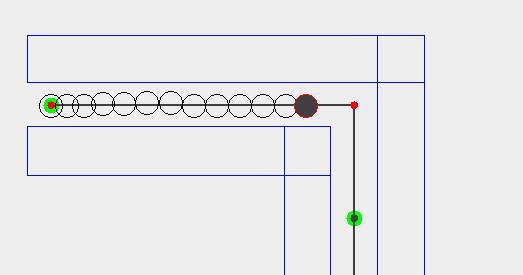
\includegraphics[width=0.65\textwidth]{small-margin-fail-post}
\caption[An example of the UAV going too fast to execute a turn]{The  UAV, represented as the filled black circle, at a transition between segments. It ended the previous segment (on the left) with a high velocity. It cannot slow down in time to turn the corner without a collision.}
\label{fig:turn-fail}
\end{figure}
The first reason is that it helps ensure that each segment can always be solved. When the UAV reaches the goal of a specific segment, it may be traveling at a high velocity. This means that it may also start the next segment at a high velocity. If this transition between segments happens right before a tight corner, the UAV may not be able to avoid a collision in the segment it is transitioning to. This is shown in Figure \ref{fig:turn-fail}.
\par
\begin{figure}
\centering
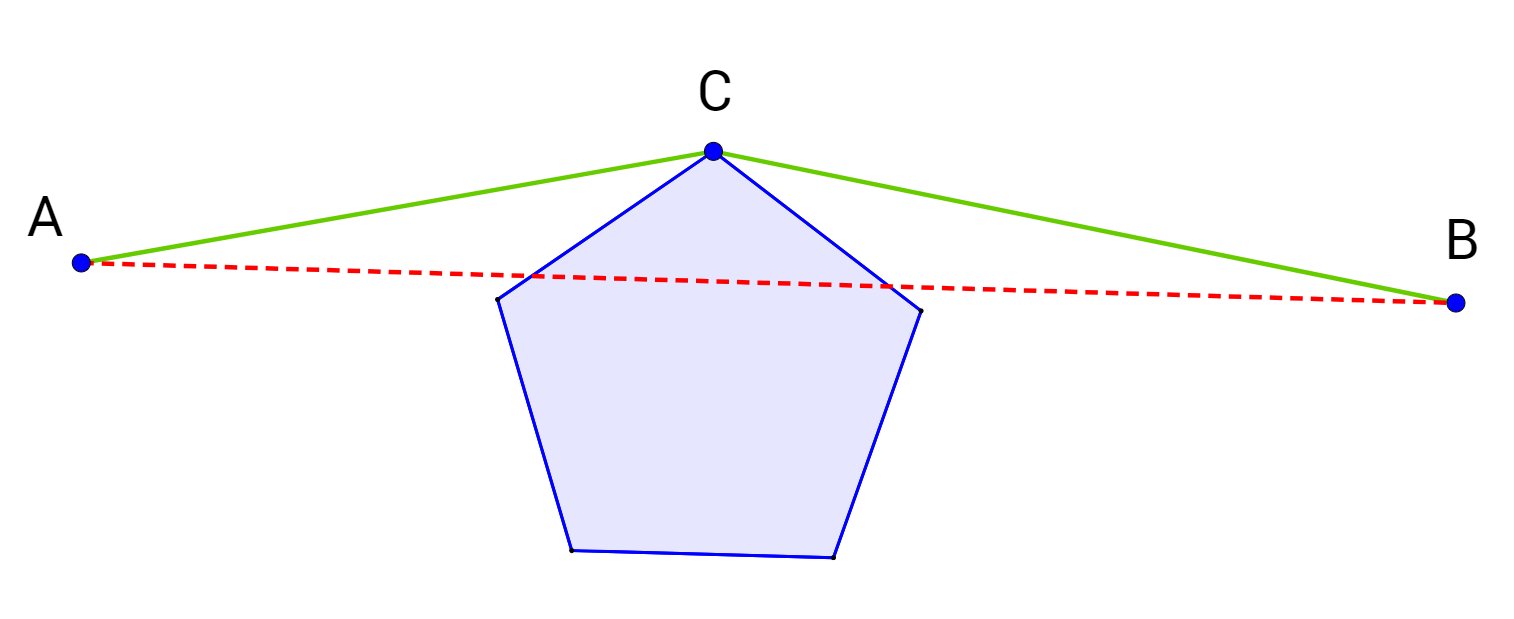
\includegraphics[width=0.65\textwidth]{inside-corner}
\caption[A demonstration of how obstacles cause turns]{The straight line path between A and B (red dashed line) is not possible because the blue obstacle is in the way. The shortest path now passes through point C (green line). The blue obstacle causes the turn in point C to exist.}
\label{fig:inside-corner}
\end{figure}
The second reason is that generating the segment around turns in the Theta* path helps improve performance. In Euclidian geometry, the shortest path between two points is always a straight line. When polygonal obstacles are introduced between those points, the shortest path will be composed of straight lines with turns at one or more vertices of the obstacles. The obstacle that causes the turn will always be on the inside of the corner. This is shown in Figure \ref{fig:inside-corner}.
\par
Turns in the Theta* path are also expressions of non-convex parts in the problem. Looking at Figure \ref{fig:inside-corner} again, points A and B are both valid positions in the search space. However, because the red line passes through an obstacle, the search space is non-convex. The red line crossing the obstacle causes both the turns and the non-convex search space. Therefore, the turns in the Theta* path can be seen as manifestations of the non-convexity of the search space.
\par
Since poor performance of any MILP is due to the non-convexity of the search space, the individual subproblems should be kept as convex as possible. By generating the segments around these turns, the algorithm can ensure that there is at most one turn per segment. This limits the non-convexity in the subproblem defined by each segment.
\par
While every node in the Theta* path (except the start and goal) coincide with a turn, they can be close together. When two or more consecutive nodes turn in the same direction (clockwise or counter-clockwise) and are close enough together, they can be considered to represent a single turn. The algorithm groups those nodes together in a turn event. Each turn event contains one or more nodes. A turn event predicts the existence of a turn in the MILP trajectory based on the   Theta* path, bridging the gap between them. This is demonstrated in Figure \ref{fig:turn-events}.

\begin{figure}
\centering
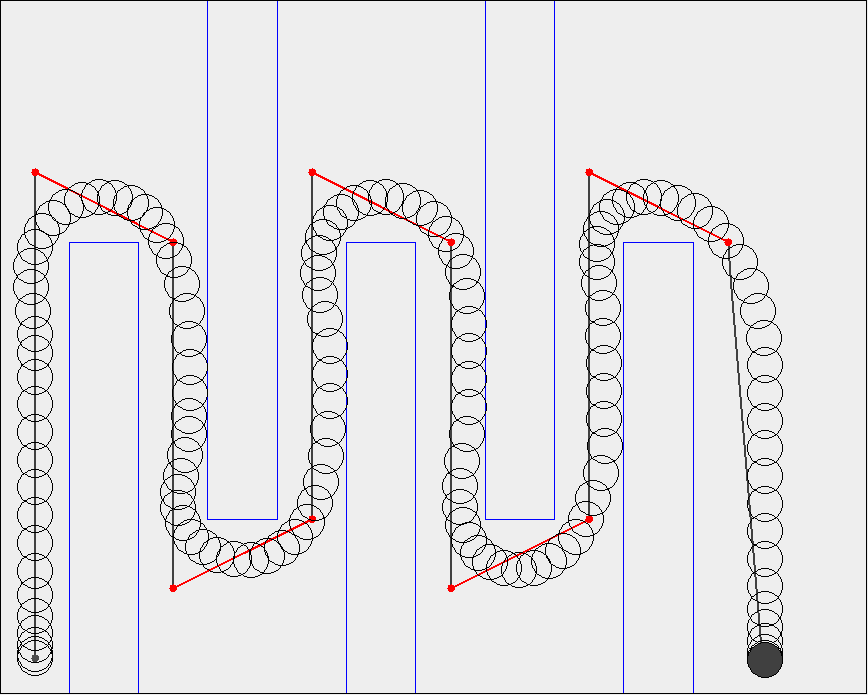
\includegraphics[width=0.65\textwidth]{turn-events}
\caption[A visualization of turn events]{This figure shows the Theta* path on the Up/Down scenario, with the turn events on that Theta* path highlighted in red. The trajectory of the UAV is also shown to illustrate how the turn events on the Theta* path match up with turns in the trajectory.}
\label{fig:turn-events}
\end{figure}
\newpage
\begin{algorithm}[t]
\caption{Finding Turn Events}
\label{alg:corners}
\begin{algorithmic}[1]
\Function{FindTurnEvents}{$path$}
  \State $\Delta max \leftarrow$ max. acc. distance * turn tolerance
  \State $events \leftarrow \{\}$ \Comment{The list of turn events found so far}
  \State $i \leftarrow 1$ \Comment{Skip the start node, it can't be a turn}
  \While{$i < |path| - 1$ } \Comment{Skip the goal node}
  	\State $event \leftarrow \{ path(i) \}$ \Comment{Start new turn event}
  	\State $turnDir \leftarrow$ \Call{TurnDir}{$path(i)$} 
    	\State $i \leftarrow  i + 1$
    	\While{$i < |path| - 1$ }
    	\If{$||path(i-1) - path(i)|| > \Delta max$}
    		\Break \Comment{Node is too far from previous}
	\EndIf
	\If{\Call{TurnDir}{$path(i)} \neq turnDir$}
		\Break \Comment{Node turns in wrong direction}
	\EndIf
	\State $event \leftarrow event \cup \{ path(i) \}$\Comment{Add to event}
	\State $i \leftarrow  i + 1$
	
    	\EndWhile
    	
    	\State $events \leftarrow events \cup \{ event \}$
  \EndWhile
\Return $events$
\EndFunction
\end{algorithmic}
\end{algorithm}

\subsection{Algorithm Implementation}
Algorithm \ref{alg:corners} processes the Theta* path to generate turn events. Two factors determine whether or not nodes are grouped together into events:
\begin{itemize}
\item The turn direction: a node $v$ in the path can either turn the path clockwise or counter-clockwise, as determined by TurnDir($v$) Two nodes with a different turn direction cannot be in the same turn event.
\item The maximum distance between two nodes in a turn event: Nodes which are too far from each other should not be merged. This distance $\Delta max$ is based on a turn tolerance parameter multiplied by the UAV's maximum acceleration distance (MAD). 
\end{itemize}



\paragraph{Maximum Acceleration Distance}
With $a_{max}$ and $v_{max}$ respectively the UAV's maximum acceleration and velocity, the time needed to reach the maximum velocity is $t_{max} = v_{max} / a_{max}$. The maximum acceleration distance is the distance traveled during that time, which equals $t_{max}^2 / 2 = v_{max}^2 / 2a_{max}$. The $MAD$ is used in several places in the algorithm as an approximation of the distance in which the UAV can recover from a maneuver. In $1*MAD$, the UAV can accelerate to any velocity from zero, or it can stop from any velocity. In $2*MAD$, the UAV can transition from any velocity vector to any other velocity vector. It is an approximation of the distance at which the presence or absence of an event can influence the UAV. \\
In this case, the MAD is relevant because turns require the velocity vector of the UAV to change from their value before the turn to a new value after the turn. If two nodes have a distance of more than $2*MAD$ between them, the turns at each node can be handled independently as distinct turns. 
\par
In the Theta* path, all but the first and last nodes are turns in the path. The second node is always the first node in a new turn event (line 5). Subsequent nodes in the path which are not too far away from the previous node (line 9) and turn in the same direction (line 12) are added to the current turn event (line 15). The maximum distance between nodes in the same turn is $\Delta max$. Once a node is found which does not belong in the event, the event is stored (line 18), a new event is created for that node (line 5) and the process repeats until no more nodes are left.


\section{Generating path segments}

Once the turn events are found, the next step is generating the segments. Each segment defines a single MILP problem whose solution is a small part of the desired trajectory. Every segment should contain at most one turn event to keep solve times low.\\
The boundaries of the segments are calculated based on the Theta* path and the turn events. For the best performance, these segments should be as small as possible. However, performance is not the only factor. Stability of the algorithm is also important. Each segment needs to be large enough so the UAV can safely approach and exit each turn. This can be guaranteed by ensuring that the start of a segment is always at least the maximum acceleration distance (MAD) before the turn event. The distance between the start of the segment and the turn event in that segment is called the expansion distance. When the expansion distance is at least $1*MAD$, the UAV can come to a complete stop before it reaches the turn. If the UAV can safely come to a stop, it can also slow down to an appropriate velocity to safely navigate the turn. Extending the segment beyond the end of the turn event also ensures that the UAV must have completely navigated the turn by the end of the segment. Ensuring that the UAV can always safely navigate a turn means that the MILP solver can always find a feasible trajectory for that segment. Because of this, ensuring  safety also ensures stability of the algorithm. \\
Increasing the approach margin beyond the minimum required for stability can improve the speed of the trajectory. An approach margin of $1*MAD$ is considered safe because the UAV can still "slam on the breaks" to slow down in time for the turn. However, a larger expansion distance gives the UAV more time and space to maneuver so it can efficiently navigate the turn. The ratio between the expansion distance and the $MAD$ is called the approach margin: $expansion distance = approach margin * MAD$. Since the $MAD$ is determined by the UAV's properties, the approach margin is used as the parameter which controls the expansion distance.


\begin{algorithm}[h]
\caption{Generating the segments}
\label{alg:segments}
\begin{algorithmic}[1]
\Function{GenSegments}{$path$, $events$}
\State $segments \leftarrow \{\}$
\State $catchUp \leftarrow true$
\State $lastEnd \leftarrow path(0)$
\For {$i \gets 0, |events| - 1 $}
\State $event \leftarrow events(i)$
\If{$catchUp$}
	%\State $segStart \leftarrow $ \Call{ExpandBackw}{$event.start$}
	%\State \Call{AddSegments}{$lastSegEnd$, $segStart$}
	%\State $lastSegEnd \leftarrow segStart$
	\State \Call{ExpandBackwards}{$event.start$} 
	\State \Call{AddSegments}{$lastEnd$,$event.start$}
	\State $lastEnd \leftarrow event.start$
\EndIf
\State $nextEvent \leftarrow events(i+1)$
\If{$nextEvent.start$ is close to $event.end$}
	\State $mid \leftarrow$ middle between $event$ \& $nextEvent$
	\State \Call{AddSegments}{$lastEnd$,$mid$}
	\State $lastEnd \leftarrow mid$
	\State $catchUp \leftarrow false$
\Else
	\State \Call{ExpandForwards}{$event.end$} 
	\State \Call{AddSegments}{$lastEnd$,$event.end$}
	\State $lastEnd \leftarrow event.end$
	\State $catchUp \leftarrow true$
\EndIf
\EndFor
\State \Call{AddSegments}{$lastEnd$,$path(|path|-1)$}
\Return $segments$
\EndFunction
\end{algorithmic}
\end{algorithm}


\subsection{Implementation}
To generate the segments, Algorithm \ref{alg:segments} considers each turn event in turn (line 5-6). $lastEnd$ is always the end of the last segment that has been generated. It is initialized with the start position of the UAV (line 4). The algorithm generates segments around turn events, but consecutive turn events may have a large distance between them. In those cases, additional segments (straight, without turns) may need to be generated to "catch up" with the start of the next turn event. When straight segments need to be inserted, the $catchUp$ flag is set to $true$. $catchUp$ starts as $true$ to catch up from the start position of the UAV to the first turn event (line 3).
\par
First, consider the case in which there is no need to catch up to generate the segment for turn event $i$. The start of the segment is the end of the last segment, $lastEnd$. The desired end of the segment is found by expanding the end of the turn event forwards along the path by a distance equal to the expansion distance. However, This may not be possible or desirable if the next turn event ($i+1$) is too close. Two events are considered close to each other if they are separated by less than three\footnote{Requiring three (instead of two) times the expansion distance as separation between turn events ensures that the segment between those turns is also at least as long as the expansion distance. This prevents some issues that can occur with very short segments.} times the expansion distance (line 13). \\
When the current turn event and the next are too close, the middle $mid$ between those turn events is used as the boundary between the segments. In this case, the current segment is generated from $lastEnd$ to $mid$ (line 14-16). The next turn event is nearby, so there is no need to catch up (line 17). \\
When there is plenty of distance between the current turn event and the next, this is not necessary. The end of the turn event $event.end$ can be expanded forwards along the path by the full expansion distance (line 19-21). There is some distance between this turn event and the next, so catching up will be required before the next event (line 22). \\
\par

Before each turn event is considered, the algorithm checks if it needs to catch up first (line 7). If so, the start of the turn event is expanded backwards along the path by the desired expansion distance (line 8). One or more straight segments are added between the end of the last segment $lastEnd$ and the (backwards expanded) start of the current event $event.start$ (line 9-10). There are no turns in those straight segments, so their size can be kept small without the risk for stability issues. Figure \ref{fig:segment-demo} on page \pageref{fig:segment-demo} shows an example of how this algorithm operates.

\begin{figure}[h]
	\centering
	\begin{subfigure}[t]{0.3\columnwidth}
        		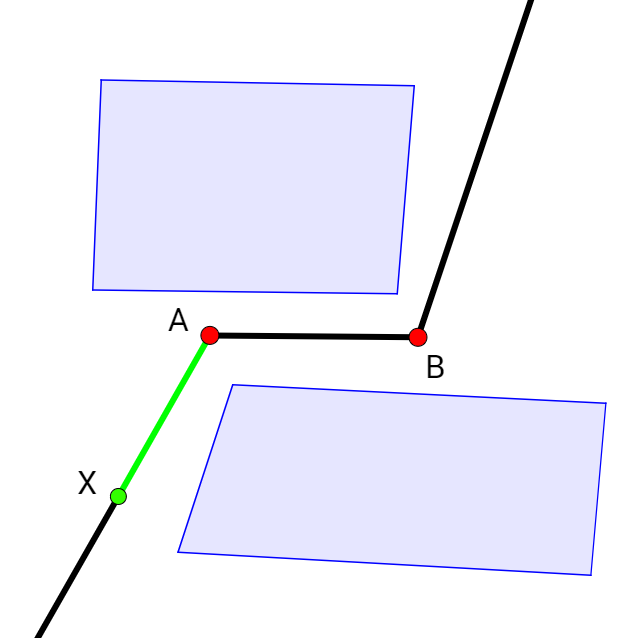
\includegraphics[width=\textwidth]{segment-xb}
        		\caption{}
        		 \label{fig:segment-demo-x}
	\end{subfigure}	
	\hfill
	\begin{subfigure}[t]{0.3\columnwidth}
        		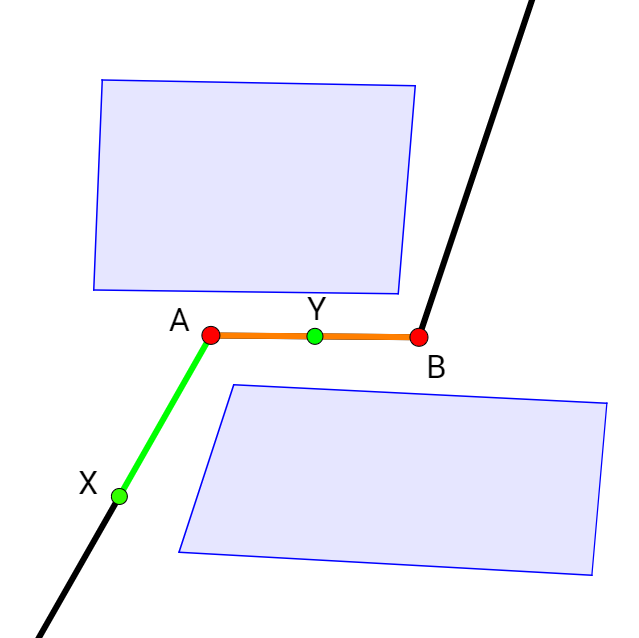
\includegraphics[width=\textwidth]{segment-yb}
        		\caption{}
        		 \label{fig:segment-demo-y}
	\end{subfigure}	
		\hfill
	\begin{subfigure}[t]{0.3\columnwidth}
        		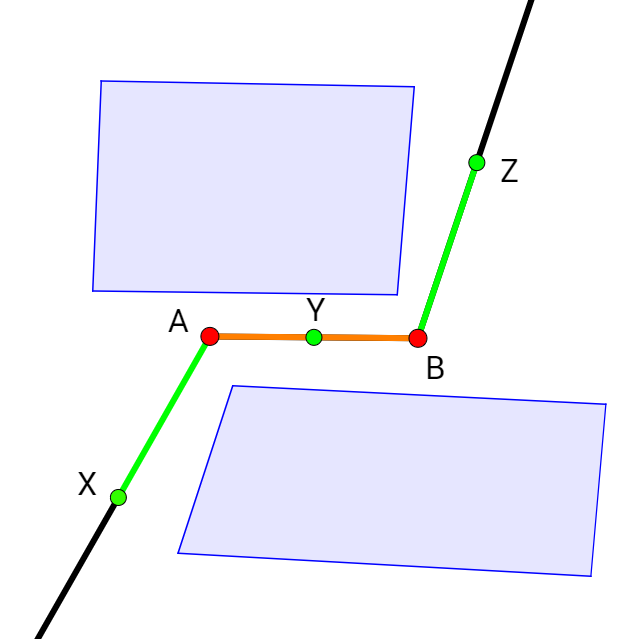
\includegraphics[width=\textwidth]{segment-z}
        		\caption{}
        		 \label{fig:segment-demo-z}
	\end{subfigure}	
	\caption[A demonstration of the segmentation algorithm]{A demonstration of the segmentation algorithm. In this example, there are two turn events at A and B as shown in red. The last segment before turn event A ends in point X, which is one expansion distance away from A. This expansion distance is marked as the green line as seen in \ref{fig:segment-demo-x}. The start position of the segment around A is X. The next step is to determine the end position of this segment. Turn event B is closer to A than the expansion distance, so the mid-point Y between A and B is chosen. This is shown in \ref{fig:segment-demo-y}, where the orange lines denote that Y is the mid-point between A and B. The segment around A is now fully constructed, starting at X and ending at Y. The next segment, around turn event B, starts in Y. There is plenty of space between B and the next turn event, so the end of the segment can be the full expansion distance removed away B, at point Z. This can be seen in \ref{fig:segment-demo-z}. The segment around B is now also fully defined, starting in Y and ending in Z. The algorithm will need to catch up to the next turn event. It will do this by adding additional straight segments which end one expansion distance before the next turn event. This leads to the situation seen in \ref{fig:segment-demo-x} as the process repeats itself.}
    \label{fig:segment-demo}     
\end{figure}

\subsection{Amount of time steps}
The amount of time steps in the MILP problem needs to be determined ahead of time. The length of the Theta* path is used to estimate how much time is needed for the UAV to reach the end of each segment. To ensure that there are always enough time steps, a conservative estimate is used. This estimate assumes that the UAV starts the segment while stopped. Afterwards, the UAV accelerates towards the turn in the segment and comes to a stop at the turn. Finally, the UAV accelerates again from the turn and stops again at the end of the segment. The time needed to complete those actions is multiplied by a multiplier parameter.

\clearpage

\section{Generating the active region for each segment}
The last step of preprocessing determines which obstacles will be modeled in the MILP problem for each segment. Segmentation already reduces the amount of time steps needed in each segment. However, modeling a large amount of obstacles still reduces the performance to unacceptable levels. \\
Not every obstacle needs to be modeled in the MILP subproblems to avoid collisions. Only the obstacles in the neighborhood around each segment are relevant. \\
Furthermore, not all obstacles in the neighborhood actually need to be modeled either. There is a fundamental difference between the obstacles on the inside of the turn and those on the outside. Obstacles on the inside of a turn are the cause for that turn. They cause the non-convex search space. Without those obstacles, the UAV could move in a straight line from the start of a segment to the goal. Therefore, obstacle avoidance for the inner obstacles must make the search space more non-convex\\
The same is not true for obstacles on the outside of the turn. Without those obstacles the optimal trajectory may have a slightly different shape, but the turn would still be there. As a result, obstacle avoidance for the outer obstacles does not necessarily have to reduce convexity. \\

\begin{figure}[h]
	\centering
	\begin{subfigure}[t]{0.45\columnwidth}
        		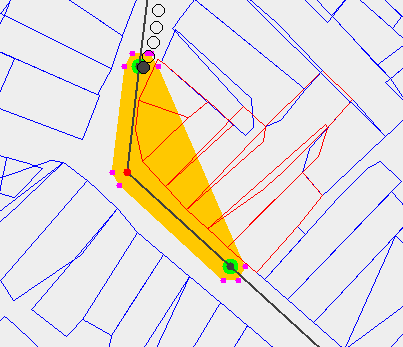
\includegraphics[width=\textwidth]{ga-seed}
        		\caption{}
        		 \label{fig:ga-seed}
	\end{subfigure}	
	\hfill
	\begin{subfigure}[t]{0.45\columnwidth}
        		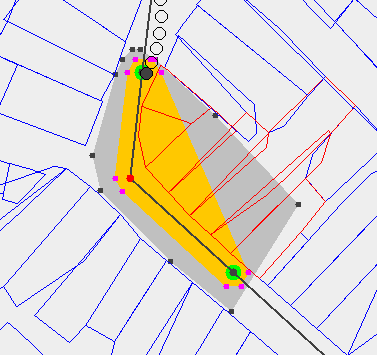
\includegraphics[width=\textwidth]{ga-seed-expanded}
        		\caption{}
        		 \label{fig:ga-seed-expanded}
	\end{subfigure}		
	\caption[A demonstration of the input and output of the genetic algorithm]{\ref{fig:ga-seed} shows the original safe region based on the convex hull of the path in orange. The obstacles that intersect this safe region are marked in red. \ref{fig:ga-seed-expanded} shows the expanded safe region as generated by the genetic algorithm in dark grey. This expanded region may not intersect any of the blue obstacles.}
    \label{fig:ga-seed-demo}     
\end{figure}

Figure \ref{fig:ga-seed} shows this difference. The obstacles on the inside of the turn are displayed in red. These are the obstacles that prevent the UAV from moving in a straight line to its goal. The other obstacles, as displayed in blue, do not prevent the UAV from moving in a straight line. As long as the UAV stays inside the orange shape, it cannot collide with any of the blue obstacles. Only the red obstacle still pose a risk. These are the obstacles that will be modeled in the MILP problem.
\par
The orange shape determines which obstacles need to be modeled. This shape is based on several important points in the segment. These points include the start position of the UAV, the goal position, and every node on the Theta* path inside the segment. Because the UAV has a physical size, these points are actually represented by regular polygons which approximate the shape of the UAV. Afterwards, the convex hull of these points/polygons is calculated using the QuickHull algorithm by Barber et al. \cite{Barber1996}. Finally, the convex hull is scale up slightly to also catch some potentially very restricting obstacles on the outside of the corner.
\par
The convex hull can be considered a safe region. If the UAV stays inside this region, it cannot collide with obstacles since any obstacle that overlaps with the safe region is modeled in the MILP problem. However, this safe region restricts the movements of the UAV more than necessary. \\
To make the safe region less restrictive, A genetic algorithm is used which attempts to expand the safe region. An example of an expanded safe region is shown in \ref{fig:ga-seed-expanded}.

\begin{algorithm}[h]
\caption{Genetic Algorithm}
\label{alg:ga}
\begin{algorithmic}[1]
\Function{GenSafeRegion}{$scenario$, $segment$}
\State $pop \leftarrow $ \Call{SeedPopulation}{}
\For {$i \gets 0, N_{gens} $}
\State $pop \leftarrow pop \cup $ \Call{Mutate}{$pop$}
\State \Call{Evaluate}{$pop$}
\State $pop \leftarrow $ \Call{Select}{$pop$}
\EndFor
\Return \Call{BestIndividual}{$pop$}
\EndFunction
\Function{Mutate}{$pop$}
\ForEach {$individual \in pop$}
\State add vertex with prob. P(add vertex)
\State OR remove vertex with prob. P(remove vertex)
\ForEach {$gene \in individual.chromosome$}
\State randomly nudge  vertex
\If{new polygon is legal}
\State update polygon
\Else
\State try again at most $N_{attempts}$ times
\EndIf
\EndFor
\EndFor
\Return \Call{BestIndividual}{$pop$}
\EndFunction
\end{algorithmic}
\end{algorithm}

\subsection{Implementation of the genetic algorithm}
A genetic algorithm is an algorithm which evolves solutions using a process inspired by natural selection in biological evolution. Genetic algorithms typically use a population of individuals which compete with each other. Each individual has a genome consisting of chromosomes, which in turn consists of individual genes. The genome determines the traits of each individual, also called the phenotype. The structure and quantity of the genes depend on the kind of problem that the genetic algorithm should solve. \\
Like in biology, the individuals can produce offspring. This offspring can be a crossover between multiple parent individuals, or a mutated version of a single parent. An important part of evolution is the concept of "survival of the fittest". A genetic algorithm improves its population by letting individuals compete. The losing individuals get eliminated from the population, while those who survive get the opportunity to create offspring. This competition is based on a fitness function. Each individual represents a possible solution for a problem. The fitness function scores the individuals based on how well they solved the problem.
\par
Algorithm \ref{alg:ga} shows the implementation of the genetic algorithm. In this implementation, each individual in the population represents a single legal polygon. A legal polygon is convex, does not self-intersect, can only overlap with the selected obstacles and contains the original safe region entirely. The latter requirement prevents the polygon from drifting off. Each individual has a single chromosome, and each chromosome has a varying number of genes. Each gene represents a vertex of the polygon.
\par
\begin{figure}[h]
\centering
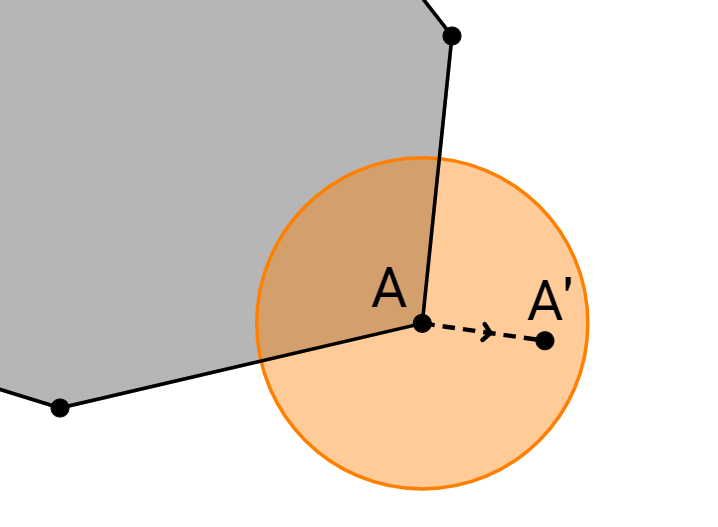
\includegraphics[width=0.45\textwidth]{genetic-mutate}
\caption[A visualization of the mutator of the genetic algorithm]{A visualization of the mutator of the genetic algorithm. The grey are is the polygon defined by the current individual. Vertex A of the individual is being mutated. The orange circle shows the maximum nudge distance. The position of the nudged vertex A' is picked at random inside this circle.}
\label{fig:genetic-mutate}
\end{figure}
The only operator is a mutator (line 4). Contrary to how mutators usually work, the mutation does not change the original individual. This means that the every individual can be mutated in every generation, since there is no risk of losing information. This mutator can add or remove vertices of the polygon by adding or removing genes (lines 12-13), but only if the amount of genes stays between a specified minimum and maximum. The mutator attempts to "nudge" every vertex/gene to a random position inside a circle around the current position (line 15). If the resulting polygon is not legal, it retries a limited number of times (line 16-19). Figure \ref{fig:genetic-mutate} shows a visual representation of this.
Tournament selection is used as the selector, with the fitness function being the surface area of the polygon (line 5-6). In tournament selection, individual compete two-by-two in each round. If an individual wins, it advances to the next round of the tournament to compete again. This is repeated until the desired population size is reached.


\clearpage
\chapter{Extensions}
\label{section:extensions}

\section{Solver-specific improvements}
The main principles that drive the algorithm work regardless of which solver is used. However, the implementation can be improved by using more specific features of the solver. For this thesis, IBM CPLEX is used as the MILP solver. This is one of the fastest, proprietary solvers available on the market. 

\subsection{Indicator constraints}
The Big M method to turn constraints on or off is functional, but there are some issues with it. M has to be big enough so it can always "overpower" the rest of the inequality. If M is too low, incorrect behavior may occur. However, if M is very large, CPLEX may have numerical difficulties or even find incorrect results \footnote{\url{http://www-01.ibm.com/support/docview.wss?uid=swg21400084}}. \\
Indicator constraints are a solution for this problem. The goal of the large M is to overpower the inequality so the constraint can be turned on or off based on a boolean variable. Indicator constraints allow constraints to be turned on or off, based on other constraints. They provide a direct way to model an "if/then" relation. Equation \ref{eq:indicator-obs} is a modified version of the obstacle avoidance constraints \ref{eq:obs-m-1-v} - \ref{eq:obs-m-4-v}. If $slack_{i,n}$ is not true, then the matching constraint on the right side must be true.

\begin{equation}
\label{eq:indicator-obs}
\neg slack_{i,n} \rightarrow \\
\begin{cases}
y_{n} -  v_i \quad \geq 
\quad a_{i} x_{n} + b_{i},  	
& \Delta q_{x,i} < 0 							 	
 \\
y_{n} + v_i \quad \leq 
\quad a_{i} x_{n} + b_{i},
& \Delta q_{x,i} > 0 							 	
 \\
x_{n} + r \quad \leq
\quad  q_{x,i}, 		
& \Delta q_{y,i} < 0, \quad \Delta q_{x,i} = 0 	
 \\
x_{n} - r \quad \geq 
\quad q_{y,i},  		
& \Delta q_{y,i} > 0, \quad \Delta q_{x,i} = 0 	
\end{cases}
\end{equation}

\subsection{Max time}
When the MILP problem is sufficiently difficult to solve, it may take a long time before the solver can find the optimal solution. To ensure an upper limit on computation time, CPLEX accepts a maximum solve time parameter. When the maximum time has expired, it will return the best solution found so far.\\
In the experiments, the maximum solve time was typically 120 seconds per segment. The goal is for every segment to be relatively easy to solve, so if no solution can be found in two minutes it counts as a failure.
\subsection{Max delta}
During testing it became clear that the solver often spends a relatively long time trying to improve trajectories which are already nearly optimal, or optimal but not yet proven to be optimal. CPLEX provides a maximum delta parameter. The delta is the difference between the best solution found so far and the upper bound for the optimal solution. If the delta is below this maximum delta, the solvers stop executing and returns the best result. When this value is small, this can reduce some of the execution time while barely changing the quality of the trajectory.

\section{Corner cutting}
\label{subsec:corner-cutting}
\begin{figure}
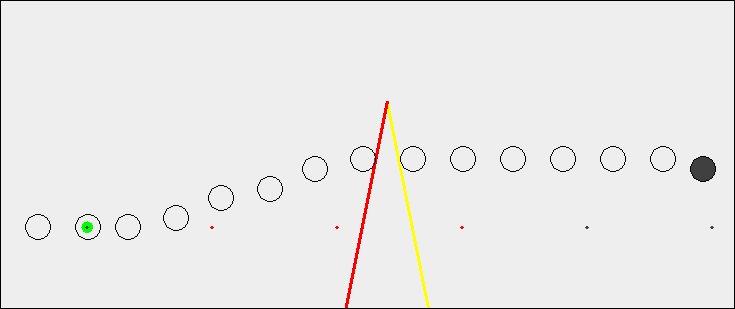
\includegraphics[width=\textwidth]{img/cornercut_bad}
\caption{An example of corner cutting}
\label{fig:cornercut-example}
\end{figure}
The MILP problem uses discrete time steps to model the changes in the UAV's state over time. An issue with this approach is that constraints are only enforced at those specific time steps. This allows the UAV to cut corners or even move through obstacles entirely if the vehicle is moving fast enough. Figure \ref{fig:cornercut-example} shows an example of this. Each time step on its own is a valid position, but a collision is ignored between the time steps.\\
Using the indicator constraint notation, Equation \ref{eq:obs-repeat-1} and \ref{eq:obs-comb-repeat-1} prevent collisions with obstacle $o$ at time step $n$. Each edge of each obstacle has an associated $slack$ variable, which determines whether or not the UAV is on the safe side for that edge.
\begin{equation}
\label{eq:obs-repeat-1}
\neg ~ slack_{i,n} \rightarrow \\
\begin{cases}
y_{n} -  v_i \quad \geq 
\quad a_{i} x_{n} + b_{i},  	
& \Delta q_{x,i} < 0 							 	
 \\
y_{n} + v_i \quad \leq 
\quad a_{i} x_{n} + b_{i},
& \Delta q_{x,i} > 0 							 	
 \\
x_{n} + r \quad \leq
\quad  q_{x,i}, 		
& \Delta q_{y,i} < 0, \quad \Delta q_{x,i} = 0 	
 \\
x_{n} - r \quad \geq 
\quad q_{y,i},  		
& \Delta q_{y,i} > 0, \quad \Delta q_{x,i} = 0 	
\end{cases}
\end{equation}
\begin{equation}
\label{eq:obs-comb-repeat-1}
\neg \mathlarger{\mathlarger{\bigwedge_{i}}} slack_{i,n} \quad 0 \leq n \leq N
\end{equation}
Richards and Turnbull\cite{Richards2015} proposed a method which prevents corner cutting. In their method, the UAV is consider on the safe side of an edge only if that is true for two consecutive time steps.  This is visualized in Figure \ref{fig:cc-fixed}. They apply the same constraints again, but this time on the position of the UAV in the last time step:
\begin{equation}
\label{eq:corner-skip-fixed}
\neg ~ slack_{i,n} \rightarrow \\
\begin{cases}
y_{n-1} -  v_i \quad \geq 
\quad a_{i} x_{n-1} + b_{i},  	
& \Delta q_{x,i} < 0 							 	
 \\
y_{n-1} + v_i \quad \leq 
\quad a_{i} x_{n-1} + b_{i},
& \Delta q_{x,i} > 0 							 	
 \\
x_{n-1} + r \quad \leq
\quad  q_{x,i}, 		
& \Delta q_{y,i} < 0, \quad \Delta q_{x,i} = 0 	
 \\
x_{n-1} - r \quad \geq 
\quad q_{y,i},  		
& \Delta q_{y,i} > 0, \quad \Delta q_{x,i} = 0 	
\end{cases}
\end{equation}
\begin{figure}
	\centering
	\begin{subfigure}[t]{0.3\columnwidth}
        		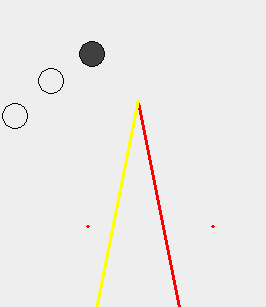
\includegraphics[width=\textwidth]{cornercut-fixed-1}
        		\caption{}
        		\label{fig:cc-fixed-1}
	\end{subfigure}
	\hfil
	\begin{subfigure}[t]{0.3\columnwidth}
        		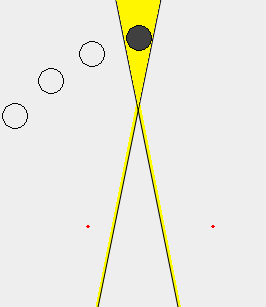
\includegraphics[width=\textwidth]{cornercut-fixed-2b}
        		\caption{}
        		 \label{fig:cc-fixed-2}
	\end{subfigure}	
		\hfil
	\begin{subfigure}[t]{0.3\columnwidth}
        		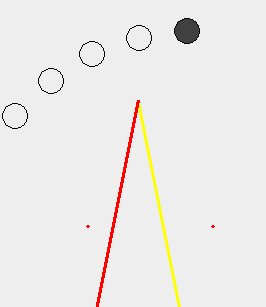
\includegraphics[width=\textwidth]{cornercut-fixed-3}
        		\caption{}
        		\label{fig:cc-fixed-3}
	\end{subfigure}
    \caption[A visual demonstration of how the corner cutting prevention works.]{These images are three consecutive time steps which demonstrate how the corner cutting prevention works. In \ref{fig:cc-fixed-1}, the UAV is in the safe region of the left edge (which is indicated by the yellow color). In \ref{fig:cc-fixed-3}, the UAV is in the safe region for the right edge, but not the left edge. To ensure that the UAV does not cut the corner, the UAV must enter the safe region of the right edge before it exits the safe region of the left edge. The intersection between those two safe regions is the inverted yellow triangle in \ref{fig:cc-fixed-2}. If the UAV spends at least one time step in that yellow, it cannot cut the corner.}
    \label{fig:cc-fixed}     
\end{figure}

\subsection{Goal conditions}
\label{subsec:goal-cond}

\begin{figure}
	\centering
	\begin{subfigure}[t]{0.45\columnwidth}
        		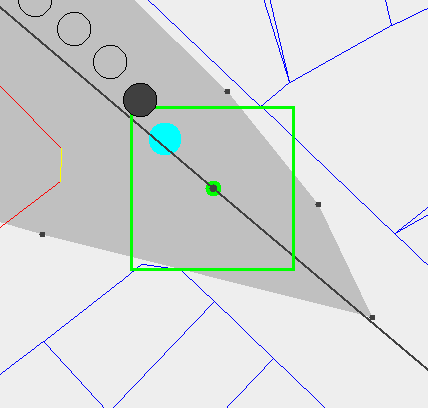
\includegraphics[width=\textwidth]{segment-pre-goal-zoom}
        		\caption{}
        		 \label{fig:goal-ext-pre}
	\end{subfigure}	
		\hfil
	\begin{subfigure}[t]{0.45\columnwidth}
        		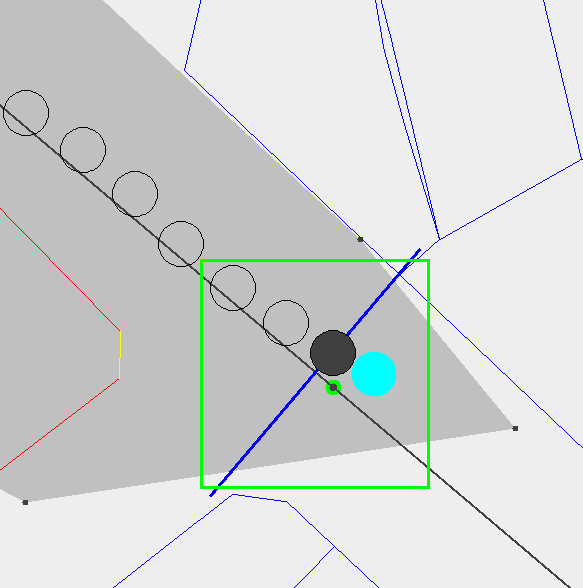
\includegraphics[width=\textwidth]{segment-extend-goal-zoom}
        		\caption{}
        		\label{fig:goal-ext-post}
	\end{subfigure}
    \caption[A visualization of the extended goal conditions]{\ref{fig:goal-ext-pre} shows the UAV right before a reaching its goal. The blue circle shows the position of the UAV at the segment transition. The goal position is the green dot, while the square around it show the tolerance region where the goal is considered to be reached. Note how the segment transition happens earlier because of the tolerance region. \ref{fig:goal-ext-post} shows the same, only this time a (blue) finish line is added. This time, the UAV needs to cross the finish line so it so the segment transition is roughly as far along the path as planned.}
    \label{fig:goal-ext}     
\end{figure}
Forcing the UAV to exactly reach each intermediate goal position is overly restrictive. Because the goal conditions are only check for each time step, the arrival at the goal position must line up with a time step. If this is not the case, the UAV could be right before the goal position on one time step, and already have passed the goal position the by the next time step. The result is that the UAV will slow down near the end of each segment so it can exactly line up with the goal position for that segment. This effect gets worse as the velocity increases.
\\
By allowing some difference between the goal position and the position of the UAV, this behavior can be resolved. However, this tolerance on the UAV's position means that the goal condition tends to be satisfied before the UAV has actually reached the goal. This is visible in Figure \ref{fig:goal-ext-pre}. By adding a finish line perpendicular to the path at the goal position and forcing the UAV to cross this line, this early finish can be counteracted. The tolerance makes the trajectory less restricted, while the finish line ensures that the segment transitions happen at the right time. This can be seen in Figure \ref{fig:goal-ext-post}.

\section{Stability Improvements}

\subsection{Maximum goal velocity}
\label{subsec:maxgoalvel}
\begin{figure}[]
	\centering
	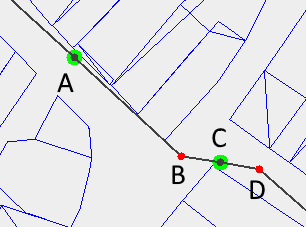
\includegraphics[width=0.5\textwidth]{goalvel}
	\caption[A scenario in which a maximum goal velocity is useful.]{A visual demonstration of when a maximum goal velocity is used. Points B and D are individual turn events. The segment for event B starts at A, with $|AB|$ being the desired expansion distance for the segment. However, because D is so close to B, the end of the segment C cannot be placed at the desired expansion distance from B. Instead, C is placed in the middle between B and D, such that $|BC|=|CD|$. The first segment solves the trajectory from A to C past turn event B, the second segment starts as C, past D and onwards. The goal is to ensure that the UAV can still safely stop at D when it starts the second segment at C. This is done by limiting the maximum velocity of the UAV when it reaches the goal C in the first segment.}
	\label{fig:max-goal-vel}
\end{figure}

When two corners are close to each other, it may not be possible to expand each corner outwards by the full expansion distance. In that case, the middle between those corners is chosen as the transition between the the segments for each corner. \\
This ensures that both corners get a fair share of the space between them. However, it breaks the assumption behind the corner expansion. If the velocity after the first corner is high, due to the reduced approach distance, the UAV may not be able to stop in time for the corner. In this situation, no solution will be found in the second segment. Figure \ref{fig:max-goal-vel} shows a situation when this may be necessary.\\
As a solution for this, the UAVs velocity at the goal of the first segment can be limited so it can stop in time for the corner in the next segment. The maximum distance at the goal of the segment is $v'_{max}$, given the actual expansion distance $dist$ in Equation \ref{eq:goalvel}. 

\begin{equation}
\label{eq:goalvel}
v'_{max} = \sqrt{2 * dist * a_{max}}
\end{equation}

\subsection{Initial Safe Region}
\label{subsec:safe-ext}
\begin{figure}
	\centering
	\begin{subfigure}[t]{0.35\columnwidth}
        		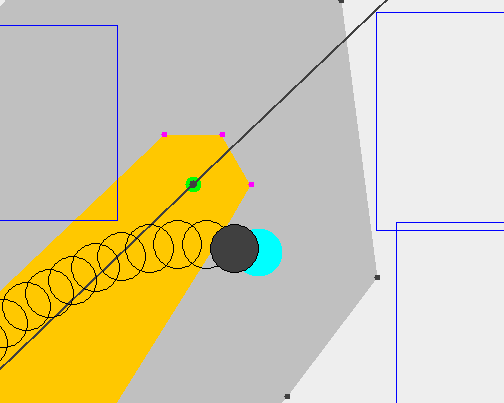
\includegraphics[width=\textwidth]{stoppoint-fail-pre}
        		\caption{}
        		\label{fig:stoppoint-fail-pre}
	\end{subfigure}
	\hfill
	\begin{subfigure}[t]{0.35\columnwidth}
        		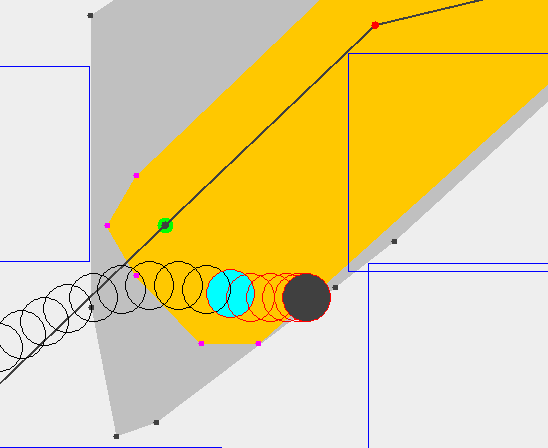
\includegraphics[width=\textwidth]{stoppoint-fail-post}
        		\caption{}
        		 \label{fig:stoppoint-fail-post}
	\end{subfigure}		
	\caption[A case in which a lack of stop point makes a segment transition fail]{An example of how transition between segments can fail. In \ref{fig:stoppoint-fail-pre}, shows the UAV right before the segment transition which happens at the blue circle. \ref{fig:stoppoint-fail-post} shows the orange initial safe region and dark grey expanded safe region of the next segment, after the transition. The next segment fails to solve because the UAV cannot come to a stop within the safe region. The position of the UAV shows where the UAV came to a stop in the previous segment (the safe region of which is the grey region in \ref{fig:stoppoint-fail-pre}).}
    \label{fig:stoppoint-fail}     
\end{figure}

The genetic algorithm is relatively simple and makes no attempt to construct the safe region such that the UAV can always stay inside it. This is problematic when the UAV has a long maximum acceleration distance. This problem presents itself in two ways.\\
The first issue arises at the start of the segment. The maximum goal velocity from section \ref{subsec:maxgoalvel} limits the UAV's velocity, but it does not determine which way the vector is pointed. The maximum goal velocity only ensures safety when the velocity vector is pointed along the path. If the velocity vector is not pointed entirely along the path, the UAV may not be able to stay within the safe region generated by the genetic algorithm. This can be seen in Figure \ref{fig:stoppoint-fail}. The solution to this issue is including the "stop point" in the initial set of points used as the safe region. This stop point is the position where the UAV would come to a halt if it starts decelerates as at the start of the segment. This depends on the initial velocity vector for that segment.\\


\begin{figure}
	\centering
	\begin{subfigure}[t]{0.30\columnwidth}
        		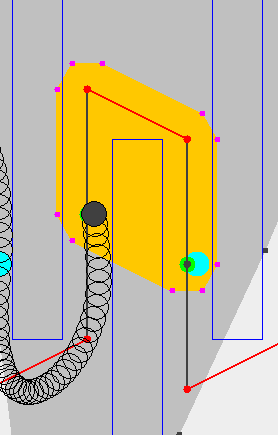
\includegraphics[width=\textwidth]{limited-ga-seed-1}
        		\caption{}
        		\label{fig:ga-seed-without}
	\end{subfigure}
	\hfill
	\begin{subfigure}[t]{0.30\columnwidth}
        		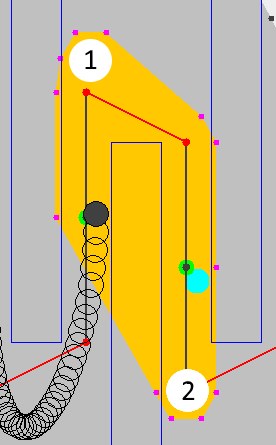
\includegraphics[width=\textwidth]{extended-ga-seed-2}
        		\caption{}
        		 \label{fig:ga-seed-with}
	\end{subfigure}	
	\hfill
	\begin{subfigure}[t]{0.30\columnwidth}
        		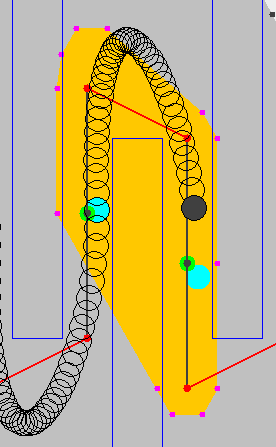
\includegraphics[width=\textwidth]{extended-ga-seed-2b}
        		\caption{}
        		 \label{fig:ga-seed-nomaxvela}
	\end{subfigure}		
	\caption[The effect of the inclusion of stop points on the initial convex safe region.]{\ref{fig:ga-seed-without} shows the initial safe region without the extra stop points in orange. \ref{fig:ga-seed-with} shows the initial safe region with the extra stop points. The position marked with "1" is the stop point for the initial velocity, while the position marked with "2" is the stop point for the trajectory after the goal has been reached. \ref{fig:ga-seed-nomaxvela} shows how the stop point ensured that the UAV could stop. The UAV leaves the initial safe region because it already has started to turn, however the stop point clearly provided enough space.}
    \label{fig:ga-seed-1}     
\end{figure}


The second issue comes into play at the end of a segment. The sub-trajectory for each segment does not end when the goal is reached. It must be calculated for all available time steps. The safe region may be very restrictive just after the UAV has reached its goal. The result is that the UAV has to slow down \emph{before} it reaches its goal to ensure the rest of the trajectory stays within the safe region. This can also by counteracted by including a stop point in the safe region. This time, the velocity vector of the UAV is not known in advance (since the segment has not been solved yet). The velocity vector is assumed to point along the path and the magnitude is either the maximum goal velocity or maximum velocity, depending on whether the maximum goal velocity is defined.\\
Figure \ref{fig:ga-seed-1} shows the result when both of these stop points are included. In the example, the maximum goal velocity has been ignored to exaggerate the effect. However, the extra stop points should always be used together with the maximum goal velocity. The stop points allow the UAV to make the transition between segments at higher velocities, but that also means they can overshoot in turns. This is demonstrated in Figure \ref{fig:ga-seed-maxvel}.

\begin{figure}
	\centering
	\begin{subfigure}[t]{0.30\columnwidth}
        		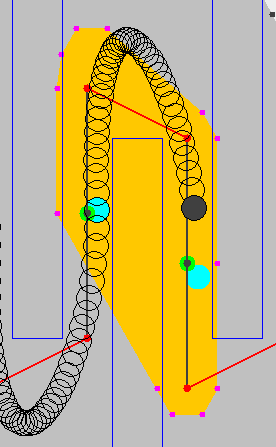
\includegraphics[width=\textwidth]{extended-ga-seed-2b}
        		\caption{}
        		 \label{fig:ga-seed-nomaxvelb}
	\end{subfigure}	
	\hfill
	\begin{subfigure}[t]{0.30\columnwidth}
        		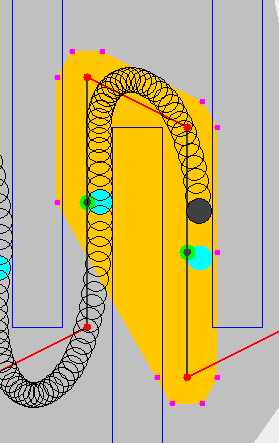
\includegraphics[width=\textwidth]{extended-ga-seed-2c}
        		\caption{}
        		 \label{fig:ga-seed-maxvelc}
	\end{subfigure}		
	\caption[A demonstration of why stop points should only be used with a maximum goal velocity.]{ \ref{fig:ga-seed-nomaxvelb} and \ref{fig:ga-seed-maxvelc} show the trajectory respectively without and with the maximum goal velocity enabled. In \ref{fig:ga-seed-nomaxvelb}, the UAV overshoots the corner which results in a slower trajectory.}
    \label{fig:ga-seed-maxvel}     
\end{figure}


\begin{figure}
	\centering
	\begin{subfigure}[t]{0.30\columnwidth}
        		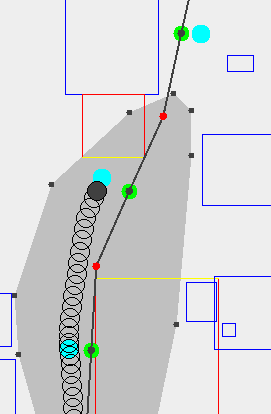
\includegraphics[width=\textwidth]{img/transition-suboptimal-pre}
        		\caption{}
        		 \label{fig:transition-suboptimal-pre}
	\end{subfigure}	
	\hfill
	\begin{subfigure}[t]{0.30\columnwidth}
        		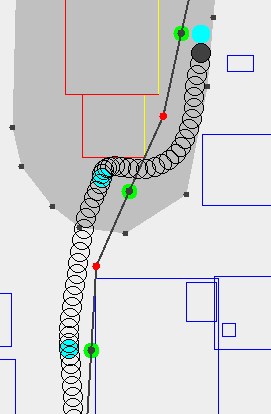
\includegraphics[width=\textwidth]{img/transition-suboptimal-post}
        		\caption{}
        		 \label{fig:transition-suboptimal-post}
	\end{subfigure}	
		\hfill
	\begin{subfigure}[t]{0.30\columnwidth}
        		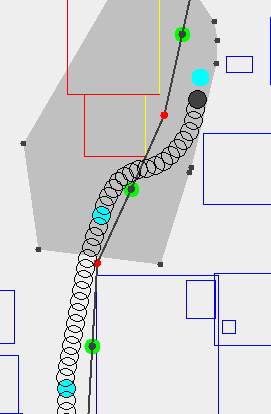
\includegraphics[width=\textwidth]{img/transition-suboptimal-fixed}
        		\caption{}
        		 \label{fig:transition-suboptimal-fixed}
	\end{subfigure}		
	\caption[A case in which overlapping segments significantly improves the quality of the trajectory]{\ref{fig:transition-suboptimal-pre} shows the optimal approach to the goal of the previous segment. However, as seen in \ref{fig:transition-suboptimal-post}, this is a very bad start state for the next segment. By starting the next segment 5 time steps earlier in \ref{fig:transition-suboptimal-fixed}, this bad approach for can be partially mitigated.}
    \label{fig:transition-suboptimal}     
\end{figure}
\section{Overlapping segment transitions}

The initial safe region extensions (section \ref{subsec:safe-ext}), more tolerant goal condition (section \ref{subsec:goal-cond}) and the maximum goal velocity (section \ref{subsec:maxgoalvel}) often improve the quality of the trajectory. However, they do not deal with all cases in which a bad segment transition happens, as demonstrated in Figure \ref{fig:transition-suboptimal}. The trajectory up to the goal of the first segment is optimal ( Figure \ref{fig:transition-suboptimal-pre}), but provides a really bad start for the next segment ( Figure \ref{fig:transition-suboptimal-post}). \\
This can be counteracted by starting the next segment earlier than usual. Instead of starting at the time step where the goal in the previous segment is reached, the next segment start several time steps earlier. This ensures the the previous segment still attempts to reach its goal as fast as possible, but also allows the next segment to correct for suboptimal transitions earlier. This can be seen in Figure \ref{fig:transition-suboptimal-fixed}.\\


\section{Graphical Visualization Tool }
\label{section:visual}
Using MILP to solve the trajectory planning problem makes my algorithm flexible. Different constraints can be added and removed without having to change complex algorithm. The solver takes those changes into account and still finds a solution.
This declarative approach makes it much easier to experiment with different variants of the problem, however it does also have downsides. One of those downsides is that it becomes harder to understand why the solution to the problem is what it is. Especially since MILP solvers don't provide a lot of useful insight during execution.\\
This problem is made worse by the fact that the trajectory planning problem is an optimization problem. We're not just interested in having any solution, but instead we want a good or possibly even the best solution.\\
These factors make the MILP solvers a "black box". This is especially problematic when they fail to find a solution. Most solvers will inform you which constraint caused the failure, but that constraint is not necessarily the one that is incorrect. Another constraint may have made the problem impossible to solve, but the solver will only fail by the time it leads to a contradiction.\\
Another problem is figuring out if all constraints are actually modeled properly. A badly modeled constraint may have no effect at all, or a different effect than intended. Gaining a deep understanding of what is happening is an issue as more and more constraints are added and the interactions between them increase.\\

\begin{figure}
	\centering
    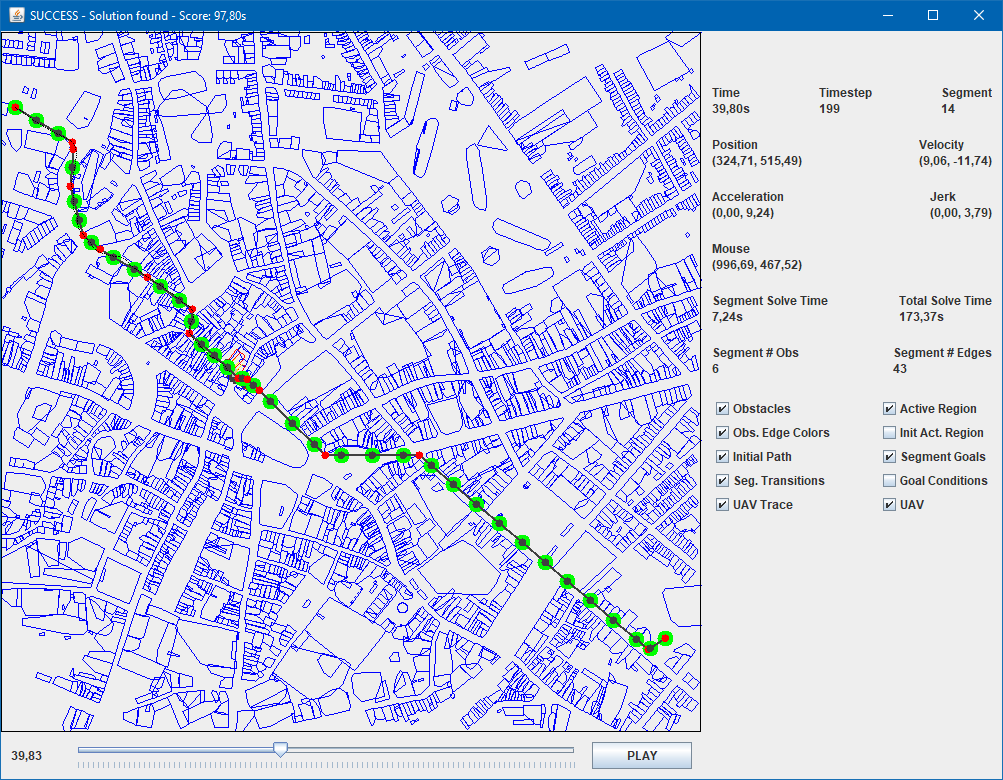
\includegraphics[width=\textwidth]{ui-full}
    \caption[An overview of the visualization tool]{An overview of the visualization tool that shows the results of the algorithm.}
    \label{fig:ui-full}     
\end{figure}

For this reason, I spent a significant amount of time building a visualization tool which displays not only the solution, but also the constraints of the MILP problem and other debugging information. This proved to be a critical part of the development cycle of the algorithm. Figure \ref{fig:ui-full} shows this tool. At first glance, the tool may look familiar. It has been used to create every example shown in this thesis. 
\subsection{Interface Elements}
The graphical interface is divided into three parts.

\paragraph{World view}The first and most prominent part is the visualization on the left. This shows a view of the world with a variety of information overlaid on top of it. The view can be translated by holding down the left mouse button and dragging around. Scrolling zooms in and out on the view.

\paragraph{Timeline}The second element is the timeline on the bottom. By dragging the slider, the user can change the time step being visualized. There is also a play/pause button which can be used to animate the visualization. The animation runs in realtime according to the progress of time of the trajectory. The animations help spot more subtle changes in acceleration which are not immediately clear from the still view.

\paragraph{Data Panel} The last element is the panel on the right. This panel contains more detailed information about the current time step being visualized. This information includes:
\begin{itemize}
\item The current time in the trajectory
\item The current time step number
\item The current segment number
\item The position, velocity, acceleration and jerk (derivative of acceleration) at the current time step
\item The world coordinates at the position of the mouse
\item The solve time for the current segment
\item The total execution time of the entire algorithm
\item The amount of obstacles and edges being modeled in the current segment
\end{itemize}
On top of that information, there are also visibility toggles for the various elements of the visualization.

\subsection{World View Elements}
\paragraph{Obstacles} The obstacles are the most common element in the visualization. Obstacles are visualized as blue polygons. See Figure \ref{fig:vis-1}.
\paragraph{Initial path} The initial path if the result of the Theta* algorithm. It is shown as black lines. The turn events on this path are red. When multiple nodes on the path belong to the same turn event, the lines connecting them are also red. See Figure \ref{fig:vis-1}.
\paragraph{Scenario goals} The scenario goals are visualized as the green circles on the initial path. These goals mark both the end of a segment and the start of the next segment. See Figure \ref{fig:vis-1}.

\begin{figure}[h]
	\centering
    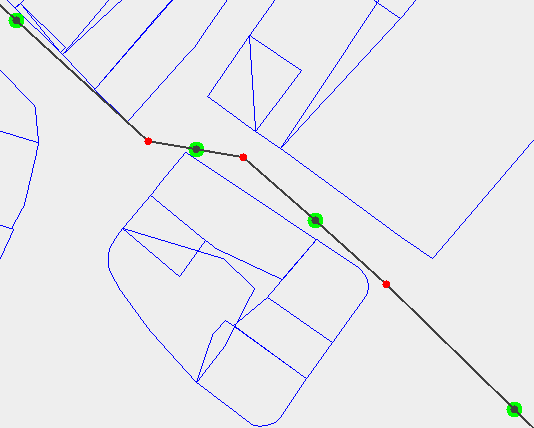
\includegraphics[width=0.7\textwidth]{vis-1}
    \caption[Visualization of the obstacles, initial path, turn events and segment goals]{The obstacles are blue, initial path is black with turn events being red. The green circles are the segment goals.}
    \label{fig:vis-1}     
\end{figure}

\paragraph{Safe region} The safe region for the current segment, the result from the genetic algorithm, is shows as a dark grey polygon. The UAV must stay within this polygon at all times. See Figure \ref{fig:vis-2}.
\paragraph{Obstacle Edge Colors} The obstacles within the safe region are modeled in the MILP problem. The color of the edges of these obstacles display whether or not the constraint is active for that edge at the current time step. If the color is yellow, the UAV is on the safe side of the obstacle. Otherwise, the color is red. See Figure \ref{fig:vis-2}.
\paragraph{Segment Transitions} The segment transitions do not always happen right at the goal positions of the segments. The light blue circle shows the position of the UAV at the time of the actual segment transition. See Figure \ref{fig:vis-2}.

\begin{figure}[h]
	\centering
    \includegraphics[width=0.7\textwidth]{vis-2}
    \caption[Visualization of the safe region, obstacle edge constrain state and the segment transitions.]{The safe region is dark grey and the segment transitions are light blue. The edges of the obstacles inside the safe region are yellow or red to signify whether or not the UAV is on the safe size of that edge.}
    \label{fig:vis-2}     
\end{figure}

\paragraph{Initial Safe Region} Before the genetic algorithm is executed, an initial safe region is constructed which ensures the UAV can reach its goal in the current segment. This initial safe region is shown in orange. The (expanded) safe region from the genetic algorithm must completely contain this initial region. See Figure \ref{fig:vis-3}.
\paragraph{Goal Conditions} The UAV does not have reach its goal exactly. The green square around the segment goal shows the tolerance region where the UAV is close enough to its goal. The blue line shows the finish line which the UAV must cross as well. See Figure \ref{fig:vis-3}.

\begin{figure}[h]
	\centering
    \includegraphics[width=0.7\textwidth]{vis-3}
    \caption[Visualization of the initial safe region and the segment goal conditions]{The initial safe region is shown in orange. To reach its goal, the UAV must be inside the green square and have crossed the blue finish line.}
    \label{fig:vis-3}     
\end{figure}
\clearpage
\chapter{Experiments and Results}
\label{section:analysis}

\section{Scenarios}
Several different scenarios are used to test the algorithm. Each scenario takes place in a world with a certain distribution of obstacles, has a start and goal position, and a UAV with certain characteristics.
\par
There are three categories of scenarios, which will be discussed in section \ref{subsec:synth} to \ref{subsec:leuven}. All scenarios are tested in a general performance test (section \ref{subsec:gen-perf}) to get an overview of the performance of the algorithm with the default parameters. This test determines whether or not the algorithm scales to large and complex environments.\\
In the other tests, only one scenario of each category has been used. Section \ref{subsec:agility} tests the performance of the algorithm as the characteristics of the UAV change. Section \ref{subsec:stability} looks at the stability of the algorithm. These tests should provide further insight into the limitations of the algorithm.\\

Sections \ref{subsec:cutting} to \ref{subsec:approach-margin} look at the effects of different parameters on both the performance of the algorithm and the quality of the trajectory. Sensible default parameters have been chosen. However, changing these parameters provides deeper insights in the characteristics of the algorithm.

All tests were executed on an Intel Core i5-4690k running at 4.4GHz with 16GB of 1600MHz DDR3 memory. The reported times are averages of 5 runs, unless stated otherwise. The machine runs on Windows 10 using version 12.6 of IBM CPLEX. The algorithm is programmed in Java 8, and uses the Jenetics 3.7 library\footnote{\url{http://jenetics.io}} for the genetic algorithm. Table \ref{table:params} on page \pageref{table:params} show the default parameters as used in all tests.

\begin{table}[h]
\centering
\begin{tabular}{ l  r | l r }
grid size 			& $2m$ 	& turn tolerance 		& $2$ \\
approach multiplier & $2$ 	& population size 		& $ 10$ \\
\# generations 		& $25$ 	& max. nudge distance 	& $5m$\\
min. \# vertices 	& $ 4$ 	& max. \# vertices 		& $12$ \\
P(add vertex) 		& $0.1$ & P(remove vertex) 		& $0.1$  \\
max nudge attempts 	& $15$ 	& $ T_{max}$ 			& $5s$ \\
time step size 		& $0.2s$& position tolerance & $3$ \\
CPLEX max solve time & $120s$ & CPLEX max delta & $1$ \\
time limit multiplier & $1.5$ & max segment time & $3s$\\
linear approx vertices & $12$ & & \\
%approach margin, maxsegment time
%fps
%pop, gens, mutrate, nudge dist, minpoints-maxpoints, addprob, removeprob
\end{tabular}
\caption{The algorithm parameters used for testing}
\label{table:params}
\end{table}
\clearpage
\subsection{Synthetic Scenarios}
\label{subsec:synth}
The synthetic scenarios have small, handmade worlds. They have few obstacles, but the obstacles are laid out in a way that makes them challenging to solve. The scenarios are shown in Figure \ref{fig:synth-scens} on page \pageref{fig:synth-scens}. There are two "Up/Down" scenarios, small (Figure \ref{fig:bench-small}) and large (Figure \ref{fig:bench-large}), in which the UAV has to move in a zig-zag pattern to reach its goal. The difference between those scenarios is the amount of obstacles, which also changes the amount of zig-zags required. These scenarios are built to see how the algorithm handles sharp turns. There is also a spiral scenario in which the UAV must go in an outwards spiral (Figure \ref{fig:spiral}).\\
The large Up/Down scenario represents this category in the tests. Table \ref{table:uav-synth} shows the properties of the UAV.

\begin{table}[h]
\centering
\begin{tabular}{ c | c | c }
$v_{max}$ ($ms^{-1}$)	& $a_{max}$ ($ms^{-2}$) 	& radius ($m$) 	 \\
\hline
$3$ & $4$ 	& $0.5$ \\
\end{tabular}
\caption{The UAV properties for the synthetic scenarios}
\label{table:uav-synth}
\end{table}

\begin{figure}
	\centering
	
	\begin{subfigure}[t]{0.5\textwidth}
        		\includegraphics[width=\textwidth]{img/bench-small}
        		\caption{The Up/Down Small Scenario}
        		\label{fig:bench-small}
	\end{subfigure}
	\par\bigskip
	\begin{subfigure}[t]{0.6\textwidth}
        		\includegraphics[width=\textwidth]{img/bench-large}
        		\caption{The Up/Down Large Scenario}
        		\label{fig:bench-large}
	\end{subfigure}	
	\par\bigskip
	\begin{subfigure}[t]{0.5\textwidth}
        		\includegraphics[width=\textwidth]{img/spiral}
        		\caption{The Spiral Scenario}
        		\label{fig:spiral}
	\end{subfigure}
        
    \caption{An overview of the synthetic scenarios}\label{fig:synth-scens}
\end{figure}
\clearpage
\subsection{San Francisco Scenarios}
\label{subsec:sf}
The San Francisco scenarios each contain a world which is based on a map of San Francisco. There are two small San Francisco scenarios (Figure \ref{fig:sf-small-1} and \ref{fig:sf-small-2}), which both share the same 1km by 1km area of San Francisco but have different start and goal locations. There is also a larger San Francisco scenario which takes places on a 3km by 3km world (Figure \ref{fig:sf-large}). \\
All obstacles in the San Francisco dataset are grid-aligned rectangles, laid out in typical city blocks. Because of this, density of obstacles is predictable. These scenarios showcase that the algorithm can scale to realistic scenarios with much more obstacles than is typically possible with a MILP approach. \\
The first small San Francisco scenario is used to represent this category in the tests. Table \ref{table:uav-sf} shows the properties of the UAV and Figure \ref{fig:sf-zoom} shows a zoomed-in view of the first small scenario. 


\begin{table}[h]
\centering
\begin{tabular}{ c | c | c }
$v_{max}$ ($ms^{-1}$)	& $a_{max}$ ($ms^{-2}$) 	& radius ($m$) 	 \\
\hline
$10$ & $15$ 	& $2.5$ \\
\end{tabular}
\caption{The UAV properties for the San Francisco scenarios}
\label{table:uav-sf}
\end{table}

\begin{figure}[h]
	\centering
	\includegraphics[width=0.8\textwidth]{sf-zoom}
	\caption{A zoomed-in view of the first small San Francisco scenario}
	\label{fig:sf-zoom}
\end{figure}


\begin{figure}
	\centering
	
	\begin{subfigure}[t]{0.46\textwidth}
        		\includegraphics[width=\textwidth]{img/sf-small-1}
        		\caption{San Francisco Small 1}
        		\label{fig:sf-small-1}
	\end{subfigure}
	\hfil	
	\begin{subfigure}[t]{0.46\textwidth}
        		\includegraphics[width=\textwidth]{img/sf-small-2}
        		\caption{San Francisco Small 2}
        		\label{fig:sf-small-2}
	\end{subfigure}	
	\par
	\begin{subfigure}[t]{0.8\textwidth}
        		\includegraphics[width=\textwidth]{img/sf-large}
        		\caption{San Francisco Large}
        		\label{fig:sf-large}
	\end{subfigure}
        
    \caption{An overview of the San Francisco scenarios}\label{fig:sf-scens}
\end{figure}

\clearpage
\subsection{Leuven Scenario}
\label{subsec:leuven}
The Leuven scenarios each contain a world based on a map of the city of Leuven. This is an old city with a very irregular layout. The dataset, provided by the local government\footnote{\url{https://overheid.vlaanderen.be/producten-diensten/basiskaart-vlaanderen-grb}}, also contains full polygons instead of the grid-aligned rectangles of the San Francisco dataset. While most buildings in the city are low enough so a UAV could fly over, it presents a very difficult test case for the path planning algorithm. The density of obstacles varies greatly and is much higher than in the San Francisco dataset across the board.\\
The first small Leuven scenario is used to represent this category in the tests. Table \ref{table:uav-leuven} shows the properties of the UAV and Figure \ref{fig:leuven-zoom} shows a zoomed-in view of the first small scenario. 
\begin{table}[h]
\centering
\begin{tabular}{ c | c | c }
$v_{max}$ ($ms^{-1}$)	& $a_{max}$ ($ms^{-2}$) 	& radius ($m$) 	 \\
\hline
$10$ & $15$ 	& $1$ \\
\end{tabular}
\caption{The UAV properties for the Leuven scenarios}
\label{table:uav-leuven}
\end{table}

\begin{figure}[h]
	\centering
	\includegraphics[width=0.8\textwidth]{leuven-zoom}
	\caption{A zoomed-in view of the first small the Leuven scenario}
	\label{fig:leuven-zoom}
\end{figure}



\begin{figure}
	\centering
	
	\begin{subfigure}[t]{0.46\textwidth}
        		\includegraphics[width=\textwidth]{img/leuven-small-1}
        		\caption{Leuven Small 1}
        		\label{fig:leuven-small-1}
	\end{subfigure}
	\hfil	
	\begin{subfigure}[t]{0.46\textwidth}
        		\includegraphics[width=\textwidth]{img/leuven-small-2}
        		\caption{Leuven Small 2}
        		\label{fig:leuven-small-2}
	\end{subfigure}	
	\par
	\begin{subfigure}[t]{0.8\textwidth}
        		\includegraphics[width=\textwidth]{img/leuven-large}
        		\caption{Leuven Large}
        		\label{fig:leuven-large}
	\end{subfigure}
        
    \caption{The Leuven scenarios}\label{fig:leuven-scens}
\end{figure}
\clearpage
\section{General Performance}
In this test, the general performance of the different parts of the algorithm are tested. Every scenario is tested with the default parameters. Table \ref{table:gen-data} shows some detailed information about the scenarios, including the length of the Theta* path and the amount of segments the problem is divided into. Table \ref{table:gen-results} shows the execution parts for the most computationally expensive parts of the algorithm (the Theta* path, genetic algorithm and MILP solver), as well as the total time required. It also shows the score of the resulting trajectories. This score is in seconds and is the amount of time that the UAV needs to reach the goal position when following the trajectory. 

\label{subsec:gen-perf}
\begin{table}[]
\centering
\begin{tabular}{ l | r | r  | l | r | r}
Scenario name & \# obs. & \# edges & world size & path (m) & \# segments \\
\hline
Up/Down Small 	& 5 	& 5 		& 25m x 20m 	& 88 	& 7   \\ 
Up/Down Large 	& 9 	& 9 		& 40m x 20m 	& 146 	& 11  \\
Spiral		 	& 11 	& 11 		& 30m x 30m 	& 96 	& 10  \\
SF Small 1		& 1235 	& 4940 		& 1km x 1km 	& 1392 	& 34  \\
SF Small 2		& 1235 	& 4940 		& 1km x 1km 	& 1490 	& 38  \\
SF Large	 	& 6580 	& 26320		& 3km x 3km 	& 4325 	& 107 \\
Leuven Small 1 	& 3079 	& 19941	 	& 1km x 1km 	& 1312 	& 34  \\
Leuven Small 2	& 3079 	& 19941		& 1km x 1km 	& 864 	& 22  \\
Leuven Large 	& 18876	& 111998 	& 3km x 3km 	& 3041 	& 78  \\
\end{tabular}
\caption{Some information about the scenarios tested.}
\label{table:gen-data}
\end{table}

\begin{table}[]
\centering
\begin{tabular}{ l | r | r | r | r || r}
Scenario name & Theta* (s) & GA (s) & MILP (s)  & total (s) & score (s) \\
\hline
Up/Down Small 	& 0.00 	& 0.33 	& 10.48 & 10.97 & 27.24	\\ 
Up/Down Large 	& 0.00 	& 0.65 	& 17.95 & 18.87 & 44.76	\\
Spiral		 	& 0.01 	& 1.06	& 7.17	& 8.46 	& 28.72	\\
SF Small 1		& 1.37 	& 7.68 	& 32.81 & 42.43 & 106.20\\
SF Small 2		& 1.82 	& 7.98	& 36.81 & 47.32 & 114.36\\
SF Large	 	& 15.88	& 15.41	& 75.44 & 108.28 & 325.10\\
Leuven Small 1 	& 1.51 	& 23.49	& 135.86& 161.85& 97.44	\\
Leuven Small 2	& 0.53 	& 14.00	& 62.03 & 76.99 & 65.52	\\
Leuven Large 	& 14.65	& 67.55	& 460.46 & 544.73 & 227.27\\
\end{tabular}
\caption{A breakdown of the execution time for each scenario, as well as the score of the trajectory.}
\label{table:gen-results}
\end{table}






\begin{table}[]
\centering
\begin{tabular}{ l | r | r | r | r | r}
Scenario name & path (m) & Theta* (s) & GA (s) & MILP (s)  & total (s) \\
\hline
Up/Down Small 	& 12.57	& 0.00 	& 0.05 	& 1.50 	& 1.57 	\\ 
Up/Down Large 	& 13.27	& 0.00 	& 0.06 	& 1.63 	& 1.72 	\\
Spiral		 	& 9.60	& 0.00 	& 0.11	& 0.72	& 0.85	\\
SF Small 1		& 40.94 & 0.04 	& 0.23 	& 0.97 	& 1.25 	\\
SF Small 2		& 39.21	& 0.05 	& 0.21	& 0.97 	& 1.25 	\\
SF Large	 	& 40.42	& 0.15	& 0.14	& 0.71 	& 1.01 	\\
Leuven Small 1 	& 38.59	& 0.04 	& 0.69	& 4.00	& 4.76	\\
Leuven Small 2	& 39.27	& 0.02 	& 0.64	& 2.82 	& 3.50	\\
Leuven Large 	& 38.99	& 0.19	& 0.87	& 5.9 	& 6.98 	\\
\end{tabular}
\caption{A breakdown of the execution time per segment}
\label{table:gen-results-rel}
\end{table}

\newpage
\subsection{Interpretation}
With the default settings, the algorithm is capable of solving all scenarios within a reasonable amount of time. In every case, solving the MILP problem takes the majority of the time. \\
The amount of segments differs between these scenarios. Table \ref{table:gen-results-rel} expresses the results relative to the amount of segments, as well as the path length per segment.
\par
A first observation is that the path length per segment is very similar for all San Francisco and Leuven segments. The UAV has the same maximum velocity and acceleration in those scenarios. Even though the density and layout of the obstacles is very different, the amount of segments scales linearly with the path length as long as the UAV properties remain the same.
\par
Another observation is that the relative time needed to calculate the Theta* path increases as the path length increases. This is not surprising since Theta*, like A*, has an exponential worst-case complexity. This means that the scalability of Theta* puts an upper limit on the scalability of the entire algorithm.
\par
The next observation is that the genetic algorithm (GA) execution times and MILP solve times are very similar within categories. For the synthetic category, the Up/Down scenarios are virtually identical in both measures. For the spiral scenario, the GA execution time is slightly higher, but the MILP solve time is lower .  \\
For the San Francisco scenarios, the two small scenarios have very similar GA and MILP execution times, but the larger scenario is actually faster per segment. The two small Leuven scenarios are also similar in GA execution time, although the first scenario has a higher MILP solve time. The large Leuven scenario has higher execution times per segment for both the GA and MILP solver.
\par
\newpage
\begin{figure}[h]
	\centering
	
	\begin{subfigure}[t]{.40\textwidth}
        		\includegraphics[width=\textwidth]{img/sf-sparse}
        		\caption{The large San Francisco scenario has a region with very sparse obstacles.}
        		\label{fig:sf-sparse}
	\end{subfigure}
	\hfil
	\begin{subfigure}[t]{.45\textwidth}
        		\includegraphics[width=\textwidth]{img/leuven-dense-2}
        		\caption{The large Leuven scenario passes through several regions with very dense obstacles}
        		\label{fig:leuven-dense}
	\end{subfigure}	
	
        
    \caption[The variations in density in different scenarios in the same world]{}\label{fig:perf-density}
\end{figure}

These variations can be explained by differences in densities between the scenarios. In the large San Francisco scenario, the trajectory crosses a region with very sparse buildings (Figure \ref{fig:sf-sparse}). The sections in the regions are easier to solve than in the smaller scenarios. The opposite happens in the large Leuven scenario, which passes through several regions with very dense obstacles (Figure \ref{fig:leuven-dense}). These account for the significant increase in execution time for both the genetic algorithm as the MILP solver.

\subsection{Comparison to pure MILP}
Comparing these results to the "pure" MILP model without preprocessing is difficult. Only the small Up/Down scenario could be solved. When given 900 seconds, the average trajectory score after 5 runs is $27.60s$. For all other scenarios, no solutions could be found even after hours of computation. The new algorithm solves the same problem in roughly $11s$, with a trajectory score of $27.24s$. The trajectory score for the pure MILP solution is worse than what  the new algorithm found, even though it is capable of finding the optimal trajectory. Finding a better solution would take even more time than the 900 seconds the solver was given.
\clearpage
\section{Agility of the UAV}
\label{subsec:agility}
The properties of the segments strongly rely on the agility of the UAV. The size of the segments is determined by the maximum acceleration distance of the UAV. \\
This experiment tests the relation between the maximum velocity and the maximum acceleration of the UAV. This test was executed on the standard set of scenarios: the large Up/Down scenario, the small San Francisco scenario and the small Leuven scenario. For each scenario I tested nine configurations of the vehicle: Every combination between three different maximum velocities and three different maximum accelerations. Table \ref{table:synth-agility} shows the different UAV properties for the Up/Down scenario, Table \ref{table:sf-leuven-agility} shows the same properties for the San Francisco and Leuven Scenarios. Table \ref{table:synth-agility-data}, \ref{table:sf-agility-data} and \ref{table:leuven-agility-data} on page \pageref{table:sf-agility-data} show the results for respectively the Up/Down, San Francisco and Leuven scenarios. Figure \ref{fig:agility-low}, \ref{fig:agility-med} and \ref{fig:agility-high} on pages \pageref{fig:agility-low}-\pageref{fig:agility-high} show the same data, but fix either the acceleration or velocity and vary the other property. \\

\begin{table}[h]
\centering
\begin{tabular}{ c || c | c | c}
 & Low & Med & High \\
\hline\hline
Velocity ($ms^{-1}$) 	& 2		& 4		& 8 	\\ 
\hline
Acceleration ($ms^{-2}$)& 1		& 3 	& 6 	\\  
\end{tabular}
\caption{The different maximum velocity and acceleration values for the vehicle for the Up/Down scenario.}
\label{table:synth-agility}
\end{table}

\begin{table}[h]
\centering
\begin{tabular}{ c || c | c | c}
 & Low & Med & High \\
\hline\hline
Velocity ($ms^{-1}$) 	& 5		& 15	& 30 	\\ 
\hline
Acceleration ($ms^{-2}$)& 3		& 10	& 20 	\\  
\end{tabular}
\caption{The different maximum velocity and acceleration values for the vehicle for the San Francisco and Leuven scenarios.}
\label{table:sf-leuven-agility}
\end{table}

\clearpage

\begin{table}[]
\centering
\begin{tabular}{ c || r | r | r}
solve time (s) & Low vel& Med vel& High vel\\
\hline\hline
Low acc 	& 26.08		& 91.98		& 100.28	\\ \hline
Med acc		& 9.93		& 16.93		& 15.17		\\  \hline
High acc	& 7.23		& 6.39		& 4.85 		\\  
\end{tabular}
\caption{Up/Down}
\label{table:synth-agility-data}
\end{table}

\begin{table}[]
\centering
\begin{tabular}{ c || r | r | r}
solve time (s) & Low vel& Med vel& High vel\\
\hline\hline
Low acc 	& 57.3		& -			& -			\\ \hline
Med acc		& 22.78		& 31.85		& 483.17	\\  \hline
High acc	& 19.53		& 13.75		& 39.64 		\\  
\end{tabular}
\caption{San Francisco}
\label{table:sf-agility-data}
\end{table}


\begin{table}[]
\centering
\begin{tabular}{ c || r | r | r}
solve time (s) & Low vel& Med vel& High vel\\
\hline\hline
Low acc 	& 127.62	& -			& -			\\ \hline
Med acc		& 64.16		& 118.86	& -			\\  \hline
High acc	& 60.83		& 53.8		& - 		\\  
\end{tabular}
\caption{Leuven}
\label{table:leuven-agility-data}
\end{table}

\subsection{Interpretation}
Several of the combinations failed to complete because the segments could not be solved within 120 seconds each. The general trend is that a higher maximum acceleration and a lower maximum velocity decrease the solve time. This is as expected, as both of those make the maximum acceleration distance smaller. A larger maximum acceleration distance leads to larger segments with more obstacles in them, which have a negative effect on the performance. 
\par
When the acceleration is high, varying the velocity has an unexpected effect. When going from a low to medium maximum velocity, the solve time actually decreases for all scenarios. I do not have an explanation for why this happens.
\par
Another slightly unexpected result is that the combination of a high maximum acceleration and high maximum velocity fails for the Leuven scenario. This is not a particularly difficult combination for the other scenarios, so the failure is unexpected.
\par
The default UAV properties seem to be right on the limit for the Leuven scenario. If the UAV is a bit less agile, the algorithm fails to find a solution. This can also be flipped on its head: the Leuven scenario is on the edge of what can be solved. The density of obstacles in the Leuven scenario is at the limit of what can be handled using the default parameters.
\begin{figure}
	\centering
	
	\begin{subfigure}[t]{\textwidth}
        		\includegraphics[width=\textwidth]{img/agility-low-speed}
        		\caption{The effects of a varying maximum acceleration and a low maximum velocity.}
        		\label{fig:agility-low-speed}
	\end{subfigure}
	\par\bigskip
	\begin{subfigure}[t]{\textwidth}
        		\includegraphics[width=\textwidth]{img/agility-low-acc}
        		\caption{The effects of a varying maximum velocity and a low maximum acceleration.}
        		\label{fig:agility-low-acc}
	\end{subfigure}	
	
        
    \caption[The low velocity and low acceleration results]{}\label{fig:agility-low}
\end{figure}

\begin{figure}
	\centering
	
	\begin{subfigure}[t]{\textwidth}
        		\includegraphics[width=\textwidth]{img/agility-med-speed}
        		\caption{The effects of a varying maximum acceleration and a medium maximum velocity.}
        		\label{fig:agility-med-speed}
	\end{subfigure}
	\par\bigskip	
	\begin{subfigure}[t]{\textwidth}
        		\includegraphics[width=\textwidth]{img/agility-med-acc}
        		\caption{The effects of a varying maximum velocity and a medium maximum acceleration.}
        		\label{fig:agility-med-acc}
	\end{subfigure}	
	
        
    \caption[The medium velocity and medium acceleration results]{}\label{fig:agility-med}
\end{figure}

\begin{figure}
	\centering
	
	\begin{subfigure}[t]{\textwidth}
        		\includegraphics[width=\textwidth]{img/agility-high-speed}
        		\caption{The effects of a varying maximum acceleration and a high maximum velocity.}
        		\label{fig:agility-high-speed}
	\end{subfigure}
	\par\bigskip	
	\begin{subfigure}[t]{\textwidth}
        		\includegraphics[width=\textwidth]{img/agility-high-acc}
        		\caption{The effects of a varying maximum velocity and a high maximum acceleration.}
        		\label{fig:agility-high-acc}
	\end{subfigure}	
	
        
    \caption[The high velocity and high acceleration results]{}\label{fig:agility-high}
\end{figure}



\clearpage
\section{Stability}
\label{subsec:stability}
\begin{figure}[]
	\centering
	\includegraphics[width=\textwidth]{stability-data}
	\caption{The data for the stability experiment}
	\label{fig:stability-data}
\end{figure}
Stability is an important property of an algorithm. When the same problem is solved several times, the algorithm should not occasionally fail to solve the problem or require a wildly different amount of time to solve that problem. \\
This experiment aims to measure the stability of the algorithm. Each of the testing scenarios is executed 50 times, instead of 5 like in the other tests. Figure \ref{fig:stability-data} shows the results of this test. The error bars show sample standard deviation. \\
\begin{figure}[h]
	\centering
	\includegraphics[width=0.5\textwidth]{transition-fail}
	\caption{A case where the transition between segments fails}
	\label{fig:transition-fail}
\end{figure}

\begin{figure}[t]
	\centering
	
	\begin{subfigure}[t]{.45\textwidth}
        		\includegraphics[width=\textwidth]{img/leuven-fail-pre}
        		\caption{This segment starts and fails with what seems like an inevitable collision...}
        		\label{fig:leuven-fail-pre}
	\end{subfigure}
	\hfill
	\begin{subfigure}[t]{.45\textwidth}
        		\includegraphics[width=\textwidth]{img/leuven-fail-post}
        		\caption{... However, this shows the trajectory in the previous segment after the goal in that segment has been reached in red. Clearly a collision is not inevitable.}
        		\label{fig:leuven-fail-post}
	\end{subfigure}	
	
        
    \caption[A demonstration that the segment transition failures are not caused by impossible starting states]{}\label{fig:leuven-fail}
\end{figure}
\subsection{Interpretation}
Even though each subproblem should ensure that the next segment can be solved, occasionally (2-4\% of the time) this was not the case as demonstrated in Figure \ref{fig:transition-fail}. It seems like a collision is inevitable, but that is actually not the case as demonstrated in \ref{fig:leuven-fail}. I believe this may be a bug in how the algorithm transitions between segments. I could not properly figure out what causes this bug.
\par
However, the algorithm does find a good trajectory in nearly all cases. When it does succeed, the standard deviation of trajectory scores are 0.6\%, 1.6\% and 0.9\% of the mean scores for the Up/Down, San Francisco and Leuven scenarios respectively. The standard deviations on execution time are higher, at respectively 13\%, 10\% and 15\% of the mean values.






\clearpage
\section{Corner cutting Prevention}
\label{subsec:cutting}
A trajectory that allows corner cutting cannot be considered safe. However, additional constraints are required to prevent this from happening. This experiment attempts to measure the impact of the corner cutting prevention. The scenarios are solved with the corner cutting mitigation from section \ref{subsec:corner-cutting} both enabled and disabled. Figure \ref{fig:corner-data} shows the results. 

\begin{figure}[]
	\centering
	\includegraphics[width=\textwidth]{corner-cutting-data}
	\caption[The results from the corner cutting prevention experiment]{The results from the corner cutting prevention experiment. The error bars show the 95\% confidence interval.}
	\label{fig:corner-data}
\end{figure}

\subsection{Interpretation}
As expected, enabling the corner cutting prevention has a negative impact on performance. This effect is limited for the Up/Down and San  Francisco scenarios. For the Leuven Scenario, the solve time more than doubles. This is likely due to the higher obstacle density and complexity.


\clearpage
\section{Linear approximation}
\label{subsec:lin-approx}
The velocity and acceleration of the UAV are limited to some finite value. Because both of those quantities are vectors, that maximum can only be approximated with linear constraints. More constraints are needed to model this more accurately which can allow for faster solutions. However, more constraints also have a performance cost. This experiment analyses the trade-off that needs to be made. The amount of vertices used for the linear approximation is tested with values of 6, 12 and 24.
\begin{figure}[]
	\centering
	\includegraphics[width=\textwidth]{linear-data}
	\caption{The results for the 2-norm linear approximation experiment.}
	\label{fig:linear-approx-data}
\end{figure}



\subsection{Interpretation}
In all cases, increasing the amount of vertices used to approximate the 2-norm also increases the solve time. The effect on trajectory score seems to be minimal for the Up/Down and Leuven trajectory. However, for the San Francisco trajectory there is a noticeable improvement with the better approximation.

\clearpage
\section{Time Step Size}
\label{subsec:timestep}
The time step size determines how many time steps are used in each MILP problem. The discretized time steps are samples at regular intervals of the continuous trajectory that the UAV would actually travel in the real world. As a result, the trajectory defined by those time steps is a piece-wise linear approximation of this smooth, real world trajectory. As the size of each step goes to zero, the approximation becomes more accurate. This also means that the trajectory should become faster, since the UAV can be controlled more precisely through time. This allows for more aggressive maneuvers. 
However, adding more time steps increases the amount of integer variables and constraints. This comes at a performance cost.
In this experiment, time step sizes of $0.1s$, $0.2s$ and $0.5s$ are tested.
\begin{figure}[]
	\centering
	\includegraphics[width=\textwidth]{timestep-data}
	\caption{The results for the time step size experiment.}
	\label{fig:timestep-data}
\end{figure}
\subsection{Interpretation}
The time step size has a dramatic impact on performance. Changing the time step size from $0.2s$ to $0.1s$ or $0.5s$ changes the solve time by a factor of 5 to 10 or even more for the Up/Down scenario. This experiment really shows the exponential complexity of MILP. Making the time steps smaller makes the algorithm much slower.
\par
As expected, decreasing the time step size also improves the score of the trajectory. The largest gain is the step from $0.5s$ to $0.2s$, although there still is some improvement when going to $0.1s$.


\section{Maximum Time}
\label{subsec:maxtime}
\begin{figure}[]
	\centering
	\includegraphics[width=\textwidth]{maxtime-data}
	\caption{The results for the segment maximum time experiment.}
	\label{fig:maxtime-data}
\end{figure}
For each subproblem, the amount of time steps to model needs to be determined in advance. The algorithm calculates an estimated upper bound for the time (and thus the amount of time steps). In the ideal case, this upper bound is equal to the time needed for the optimal trajectory. However, if the upper bound is too low, no solution can be found.\\
This experiment looks at the importance of a low upper bound on the time needed. By default, the estimated upper bound is multiplied by 1.5 to ensure enough time steps are available. A time limit multiplier of 1 is also tested, along with a multiplier of 2. 

\subsection{Interpretation}
The time needed to solve the scenarios is heavily influenced by maximum time given. For these scenarios, the default multiplier of 1.5 seems unnecessary and could be lowered to 1 without issues. Increasing the multiplier to 2 nearly doubles the solve time across the board.


\clearpage
\section{Approach Margin}
\label{subsec:approach-margin}
\begin{figure}[]
	\centering
	\includegraphics[width=\textwidth]{approach-data}
	\caption{The results for the approach margin and segment overlap experiment.}
	\label{fig:approach-data}
\end{figure}
The approach margin determines have far turn events are expanded outwards to create the boundaries between segments. A value of 1 is the minimum safe value and ensures that in the worst case, the UAV can just barely come to a stop before a turn. Higher values give the UAV more space to maneuver so more efficient approaches are possible. This experiment looks at 3 different values for the approach margin: $1.1$, $2$ and $3$. \\
Additionally, it also looks at the effect of overlapping the segments. Usually, the segments only overlap by 1 time step: the time step in which the UAV reaches the goal in the previous segment, which is the starting state for the next segment as well. Since the overlap also helps to improve the efficiency of the approach of the UAV, a scenario was tested in which 5 time steps overlap between segments with an approach margin of $1.1$.

\subsection{Interpretation}
As expected, a higher approach margin leads to a higher solve time. Larger segments tend to include more obstacles and need more time steps, negatively impacting performance. For the Up/Down scenario there is a small decrease in solve time with a margin of $3$ compared to $2$, which I cannot explain. The San Francisco scenario sees a steady increase in solve time as the approach margin is increased. This is the same for the Leuven scenario when going from a margin of $1.1$ to $2$, but between $2$ and $3$ there is a large leap in solve time. This is likely caused by the higher density of obstacles. \\
The low approach margin of $1.1$ with an overlap of 5 time steps results in the highest solve time for all 3 scenarios. This is unexpected, because a higher approach margin pushes the start of segments back more than the extra 4 time steps. More thorough analysis of where the slowdown occurs is necessary to fully understand this.
\par
In the Up/Down and San Francisco scenarios, going from an approach margin of $1.1$ to $2$ results in a clear improvement in the trajectory score. The Leuven scenario also shows an improvement, but the difference is smaller. Increasing the margin even more to $3$ has no significant effect on any scenario. Overlapping the segments results in a large improvement in trajectory scores for the San Francisco and Leuven scenario, scoring the best out of all combinations. Overlapping segments seems to be more computationally expensive, but also more effective than having a high approach margin. 
%\clearpage
%\section{Genetic Algorithm Parameters}
%\label{subsec:ga-params}

\clearpage
\chapter{Discussion}
\label{section:discussion}
The main focus points during this thesis were the performance and stability of the algorithm. Most decisions were made with either performance or stability in mind, and often both. The performance and stability of the algorithm are discussed in section \ref{subsec:disc-perf} and \ref{subsec:disc-stab} respectively. Some important parameters and their impact on the algorithm are also discussen in \ref{section:imp-params}.
\section{Performance}
\label{subsec:disc-perf}
On the performance side, it is clear that the new algorithm with preprocessing is much faster than solving the pure MILP problem without preprocessing. Comparing the new algorithm to the pure approach is difficult since the challenging scenarios for the new algorithm simply cannot be solved with the pure approach.
\par
When it comes to scalability, there are a few noteworthy observations to make. 
\subsection{Path Length Scalability}
The first is that the time needed to solve each MILP subproblem does not depend on the length of the trajectory or the size of the world. Accounting for variations due to obstacle density, the average MILP solve times for scenarios using the same data set (San Francisco or Leuven) are very similar. Since the amount of segments scales linearly with the path length, the MILP part of the algorithm also scales linearly with the length of the initial path. This is in stark contrast with the exponential worst-case performance of the pure MILP approach.\\
However, this exponential complexity has not been eliminated. It has been shifted to the initial path planning algorithm: Theta*. This algorithm still has exponential worst-case complexity with respect to the length of the path. While Theta* does limit the scalability regarding the size of the world, it is a much easier problem to solve. It is part of the A* family of path planning algorithms which have been the subject of a large body of research.
\par
The algorithm separates the "routing" aspect from the trajectory planning aspect of the problem. The exact properties of the initial path are not very important. What matters is that it determines where and when to turn. By the time the MILP solver runs, the navigation aspect of the problem has already been solved. The MILP solver only needs to find a viable trajectory. The two aspects of the problem are solved separately, making both of them easier to tackle.
\par
The realization that these two aspects can be solved separately is the key insight that makes the performance improvements possible. Solving these aspects separately means that the optimal trajectory is unlikely to be found. However, at this point this seems like a necessary sacrifice for long term trajectory planning through complex environments. I could not find any algorithm in the literature that scales as well as my algorithm does, and is capable  of finding the optimal trajectory.

\subsection{Obstacle Density Scalability}
The second observation is that the density of the obstacles plays a large role in the scalability of the algorithm. The San Francisco and Leuven scenarios are very similar, except for their obstacle density. The Leuven scenario has a significantly higher density of obstacles and is also much harder to solve. Without preprocessing, the scalability of the MILP problem is limited by the total amount of obstacles. Because each MILP subproblem in my algorithm is roughly the same size, the total amount of obstacles is no longer the limiting factor. The density of the obstacles is the limiting factor in my algorithm.
\par
The Leuven scenarios can still be solved in an acceptable amount of time, but I do not believe this will be the case if the density is increased even more. Luckily, the Leuven data set is more detailed than it needs to be. Each building in the city is represented separately, even when multiple buildings are connected. It should be possible to reduce the obstacle density substantially with a minimal amount of effort. Figure \ref{fig:leuven-dense2} shows a dense region in the Leuven dataset where there is a lot of room for improvement.

\begin{figure}[h]
	\centering
	\includegraphics[width=0.5\textwidth]{leuven-dense}
	\caption{One of the denser regions in the Leuven dataset}
	\label{fig:leuven-dense2}
\end{figure}

Given that the Leuven data set is so unoptimized for this purpose and the algorithm still only needs, on average, a few seconds per segment, I believe that the scalability with regards to the obstacle density is acceptable.

\subsection{UAV Agility} 
The last observation is the importance of the agility of the UAV. The algorithm was developed with high-end consumer to professional grade multirotor UAVs in mind. These are very agile vehicles capable of impressive feats of acrobatics when properly piloted. This agility is one of the assumptions this algorithm is based on. The UAV must be able to hover and accelerate quickly.
\par
The results from the UAV agility experiment in section \ref{subsec:agility} show that these assumptions are indeed a critical part of the performance of the algorithm. The algorithm fails when faced with UAVs with an (unreasonably) low agility. 
\par
This reliance on agility is one of the factors that made the dramatic improvement in performance possible, but it also limits the applicability of the algorithm. However, the goal of this thesis was not to developed a general algorithm. The algorithm performs well for reasonable estimates of the agility of a multirotor UAV. On top of that, the agility of any UAV can be increased by limiting its maximum velocity\footnote{Limiting the maximum velocity of UAVs with a low acceleration when navigating through a city seems like a wise decision anyway. Such a UAV would not be able to react to unexpected obstacles quickly, so having it fly at a high velocity through the city seems like a dangerous proposition.}.


\section{Stability}
\label{subsec:disc-stab}
For the algorithm to be useful, it must be stable. The first aspect of stability is whether or not it can find a solution. If the algorithm is capable of finding a solution, it should find that solution every time. It should also be able to solve problems with a similar difficulty as well. The second aspect is that the solution for the same problem should always be similar. There should be no large differences in the trajectory scores when the same problem is solved multiple times, nor should there be a large difference between similar problems. This is also applies to the execution time. The execution time for similar problems should also be similar without large variations.
\par
The new algorithm can find a solution most of the time. Due to what I believe to be a bug, it occasionally fails to find a solution. I was not able to fully understand why the bug occurs, but I believe it can be fixed.  
\par
The stability of the trajectory scores is excellent. All trajectories found are scored within a few percentage points of each other. When it comes to the execution time, there is more variation. However, with a standard deviation around 10-15 \% of the mean execution time, I believe that the stability is still acceptable for offline trajectory planning.

\section{Important parameters}
\label{section:imp-params}
During development of the algorithm I settled on sensible default parameters which balance both the performance of the algorithm and the quality of the resulting trajectory. The experiments which tested different values for those parameters provide a deeper insight in the effects of those parameters. Many of those insights point to possible improvements to the current algorithm.

\subsection{Time Step Size and Maximum Time}
In the time step size experiment (section \ref{subsec:timestep}) and maximum time experiment (section \ref{subsec:maxtime}) it becomes clear that the amount of time steps in each segment has a very large effect on the performance of the algorithm. The time step size should be chosen such that the quality of the trajectory is high enough to be usable, without being more detailed than necessary. How large the time step size should be will depend on the specific use case. The maximum time should always be as low as possible, while still ensuring that the goal can be reached in that time. \\
By combining the effects of those parameters, the algorithm could be made faster without suffering a quality penalty. For each  segment, the algorithm could first solve a MILP problem with a conservative maximum time and a large time step size. The solution to this problem shows how much time the UAV needed to reach its goal in that segment. This value can be used as a much tighter maximum time in a MILP problem with a smaller time step size. While I did not have time to properly implement this, a quick-and-dirty test showed promising results.  Using this method and solving the segments first with a time step size of $0.5s$, the San Francisco scenario MILP solve time dropped from 32s to 10s. For the Leuven scenario the MILP solve time dropped from  136s down to 38s. In both cases, the execution time was cut by more than two thirds without impacting the quality of the trajectory.
\paragraph{Divide and Conquer}
This fits in well with the "divide and conquer" approach used throughout the thesis. Not only is the trajectory planning problem solved as many smaller sub-trajectories, but the algorithm also divides the kinds of problems that need to solved. The usage of Theta* separates the routing problem from the actual trajectory planning problem. The extension suggested here separates the optimization aspect from the trajectory planning problem for the most part. The tight time estimation provided by the coarse solution ensures that any viable trajectory in the fine MILP problem is necessarily also close to the optimal trajectory. Most of the optimization already happened in the coarse MILP problem.
\par
Further exploiting this divide and conquer approach will probably lead to even more improvements. Maybe it is possible to look at the slack variables of the edges of obstacles in the coarse solution and reduce the amount of edges which need to be modeled in the fine MILP problem? Maybe the motion of the UAV in the coarse trajectory can be used to place the transitions between segments in better locations? There are many possibilities which could be explored.

\subsection{Approach Margin}
The approach margin experiment (section \ref{subsec:approach-margin}) shows that having some approach margin is beneficial, but that the gains are often relatively small. Overlapping the segments by just 5 time steps already results in a significantly better trajectory than a very large approach margin. Because of this, I believe that the idea that a larger approach margin leads to more efficient approach is not accurate. I suspect that the slight improvements in trajectory score when increasing the approach margin are caused by simply having fewer segments. Or to put it more accurately: it is caused by having fewer transitions between segments. Overlapping the segments smooths out bad transitions between those segments. A larger approach margin does not improve bad transitions, it only guarantees that the UAV can correct for it in time. These bad transitions are not immediately obvious when the UAV is constantly maneuvering, but they become very clear when the UAV is flying straight. Figure \ref{fig:sf-wavy2} shows a case where the UAV is not moving entirely along the path after a turn. This is corrected, but it starts an oscillation along the trajectory that takes many segments to die down. In Figure \ref{fig:sf-wavy2b}, the slight overlap of the segments prevents that oscillation from starting in the first place. 
\begin{figure}[h]
	\centering
	
	\begin{subfigure}[t]{.4\textwidth}
        		\includegraphics[width=\textwidth]{img/sf-wavy2}
        		\caption{}
        		\label{fig:sf-wavy2}
	\end{subfigure}
	\hfill
	\begin{subfigure}[t]{.4\textwidth}
        		\includegraphics[width=\textwidth]{img/sf-wavy2b}
        		\caption{}
        		\label{fig:sf-wavy2b}
	\end{subfigure}	
	
        
    \caption[The effect of overlapping obstacles on oscillations in the trajectory]{Without overlapping the segments, oscillations tend to occur in the trajectory as seen in \ref{fig:sf-wavy2}. Even a small amount of overlap is an effective countermeasure as seen in \ref{fig:sf-wavy2b}.}
    \label{fig:sf-wavy}
\end{figure}
With the current algorithm there is a high performance cost involved with overlapping the segments. However, I do not believe this necessarily has to be the case. This is definitely something to look at in future work.

\subsection{Genetic Algorithm}
The genetic algorithm is the part of the thesis that got the least attention. This is mainly because the genetic algorithm itself is not an essential part of the trajectory planning algorithm. It is used to grow the convex safe region, and the current genetic algorithm does that well enough. Due to time constraints I have omitted detailed parameter tuning of this genetic algorithm.
\par
Either way, the genetic algorithm is very crude. A genetic algorithm was chosen to grow the convex safe region because it is a quick way to get a reasonably good result.  Since it never was the most pressing issue in the project, it never got replaced by a more refined algorithm (genetic or otherwise). 



\clearpage
%\chapter{Degree of Non-convexity}
TODO: intro
\begin{figure}
	\centering
	\begin{subfigure}[t]{1\columnwidth}
        		\includegraphics[width=\textwidth]{small-bench-flat}
        		\caption{The horizontal scenario.}
        		\label{fig:convex-straight}
	\end{subfigure}
	\par\bigskip
	\begin{subfigure}[t]{1\columnwidth}
        		\includegraphics[width=\textwidth]{small-bench-diag}
        		\caption{The diagonal scenario.}
        		 \label{fig:convex-diag}
	\end{subfigure}	
	\par\bigskip
	\begin{subfigure}[t]{0.8\columnwidth}
        		\includegraphics[width=\textwidth]{small-bench}
        		\caption{The Up/Down Scenario.}
        		 \label{fig:convex-full}
	\end{subfigure}	
    \caption{Three different testing scenarios, each with the same amount of obstacles. In each scenario, the UAV needs nearly the same amount of time steps to reach its goal. The only difference is the layout of the obstacles.}
    \label{fig:benchmarks}     
\end{figure}

\section{Scenarios}
\label{subsec:naive-scenarios}
\begin{figure}[]
	\centering
	\includegraphics[width=\textwidth]{naive-performance}
	\caption{Performance of the MILP problem.}
	\label{fig:naive-performance}
\end{figure}
Typically, the amount of integer variables is used as a metric for the difficulty of a MILP problem. The amount of integer variables determines the worst case time needed to solve the MILP problem. An integer variable is needed for every edge, for every obstacle, for every time step. Increasing the amount of time steps and obstacles also increases the time needed to solve.\\
However, the amount of integer variables does not seem to be the only factor that determines the solve time. Figure \ref{fig:benchmarks} shows three different scenarios, each with the same amount of obstacles. The time step size is $0.2s$, and in each scenario there were 30 seconds worth of time steps. The scenarios are built such that the time needed for the UAV to reach the goal position is roughly the same (between 26 and 27 seconds). As a result, each scenario has the same amount of integer variables. With 4 edges for all 5 obstacles and 150 time steps, they each have 3000 integer variables to model the obstacles alone.\\

In the Horizontal scenario, the obstacles are not in the way of the UAV. The UAV can move in a straight line from the start position to its goal. In the Diagonal scenario, two of the obstacles are slightly in the way. The UAV is forced to make slight turns near the start and end of the trajectory. However, most of the trajectory is still straight. In the Up/Down scenario, the vehicle has to slalom around every obstacle.\\
\section{Results}
\label{subsec:naive-results}

Each scenario was solved five times. Figure \ref{fig:naive-performance} shows the time needed to solve the models, as well as the score. The score is also expressed in seconds, and is the time needed for the UAV to reach the goal position when following the generated trajectory. \\
The time needed to solve these scenarios varies dramatically. The Horizontal scenario is solved consistently in just under 3 seconds. The Diagonal scenario comes in at around 20 seconds, although the 95\% confidence interval is $\pm 4.9s$. The Up/Down scenario was limited to 900s of execution time. In this time, the solver could not find the optimal trajectory, which is why the score has a confidence interval.
\section{Discussion}
\label{subsec:naive-discussion}
Intuitively, it is not surprising that the Up/Down scenario is harder to solve than the other two. A human pilot would also have more difficulties navigating the Up/Down scenario compared to the others. However, this is cannot be determined by looking a the amount of integer variables or constraints alone.\\
Problems where the trajectory requires maneuvers seem to be harder to solve. The maneuvers are necessary because there are obstacles blocking a straight approach to the goal position. This observation led me to believe that the integer variables themselves do not cause the poor performance, but the real issue is what they model: a non-convex search space.\\
The amount of integer variables determines the worst-case performance because it determines the degree to which the search space can be non-convex. An informal definition of this degree of non-convexity would be the minimum amount of (possibly overlapping) convex shapes needed to reconstruct the original shape. With a single boolean variable, you need at most 2 convex shapes. With $n$ boolean variables, at most $2^n$ convex shapes are needed. TODO: cite.\\
\begin{figure}
	\centering
	\begin{subfigure}[t]{0.47\columnwidth}
        		\includegraphics[width=\textwidth]{small-bench-diag-convexity}
        		\caption{8 convex regions are needed to reconstruct the diagonal scenario.}
        		 \label{fig:convex-diag-convexity}
	\end{subfigure}	
	\hfill
	\begin{subfigure}[t]{0.47\columnwidth}
        		\includegraphics[width=\textwidth]{small-bench-convexity}
        		\caption{11 convex regions needed to reconstruct the Up/Down Scenario.}
        		 \label{fig:convex-full-convexity}
	\end{subfigure}	
    \caption{}
    \label{fig:benchmarks-convex}     
\end{figure}
The degree of convexity of the open space for the Up/Down scenario is 11 as shown in Figure \ref{fig:convex-full-convexity}. For the Horizontal and Diagonal scenarios, this is 8 as shown in Figure \ref{fig:convex-diag-convexity}. There is a difference, but this still does not seem like a good explanation. The Horizontal and Diagonal scenarios have the same degree of convexity, even though there's almost an order of magnitude difference in the solve times. \\
Even though the global degree of convexity is the same for the Horizontal and Diagonal scenarios, this is not the case for the neighborhood around the trajectory. In the Horizontal scenario, the trajectory only goes through a single convex region. In the Diagonal scenario, the trajectory goes through 3 convex regions. For the Up/Down scenario, the trajectory goes through all 11 regions. I present the following hypothesis:
\begin{hyp}
The degree of non-convexity around the optimal trajectory is a better indicator of the time needed to solve a MILP trajectory planning problem than the amount of integer variables.
\label{hyp:nonconvex}
\end{hyp}

%\subsection{Implications for the thesis}
%\label{subsec:naive-implications}
%While I present Hyptothesis \ref{hyp:nonconvex} before my algorithm, I actually only came up with it near the end of the project when the algorithm was already completed. The development of the algorithm was based on a lot of trial and error, exploiting the ideas that work and ignoring those that do not. MILP solvers are black boxes, so it is hard to predict which ideas will work and which do not. It is not uncommon for mathematically equivalent constraints to have drastically different effects on solve time. \\
%However, near the end of the project I started to understand the behavior of the solver better. Hypothesis \ref{hyp:nonconvex} is the result of what I have learned during the project. It is what I believe to be the core reason why my algorithm is effective.
%\par
%Section \ref{section:segment} often refers back to this hypothesis to motivate certain decisions. However, the hypothesis was often not the actual motivation behind those decisions. The arguments I present in section \ref{section:segment} are the arguments I believe to be correct at the time of writing.
%\par
%Due to time constraints, this thesis does not investigate Hypothesis \ref{hyp:nonconvex}. The outcome and conclusions of this thesis do not depend on this hypothesis

%\clearpage


\chapter{Conclusions}
\label{section:conclusions}
In this thesis, I presented a scalable trajectory planning algorithm using Mixed-Integer Linear Programming (MILP). This algorithm is capable of generating trajectories through environments on the scale of cities in 2D space. These environments can be on the order of square kilometers in size with trajectories spanning several kilometers. Previous approaches with MILP trajectory planning were not scalable enough to generate trajectories through such environments.
\par
This improvement of performance is achieved by using several steps of preprocessing. This preprocessing approach is the main contribution of this thesis to the field. During preprocessing, a Theta* path planning algorithm is used to find a viable route to reach the goal. Based on this path, the trajectory planning problem is divided into many subproblems or segments, each of which solve a small part of the final trajectory. The segments are solved consecutively and their results are stitched together to form the final trajectory.
\par
Dividing the trajectory planning problem reduces the amount of time steps and obstacles that have to be modeled in each subproblem. Minimizing both those properties is critical to ensure the MILP subproblem can be solved quickly. Special care was taken to ensure that the transitions between the segments do not cause the algorithm to fail.
\par
The algorithm was tested with a variety of scenarios. Several of those scenarios are based on maps of actual cities, namely San Francisco and Leuven. The results show that the MILP part of the algorithm scales linearly (instead of exponentially) with the trajectory length and is dependent on the density of the obstacles instead of the total amount of obstacles. The Theta* algorithm still scales exponentially, but is a much easier problem to solve with a large body of research detailing possible improvements.
\par
Detailed analysis of the effects of some of the parameters have shown that there is still a lot of room for improvement for the algorithm. 

%Path planning using MIP was previously not computationally possible in large and complex environments. The approach presented in this paper shows that these limitations can effectively be circumvented by dividing the path into smaller segments using several steps of preprocessing. The specific algorithms used in each step to generate the segments can be swapped out easily with variations. Because the final path is generated by a solver, the constraints on the path can also be easily changed to account for different use cases. The experimental results show that the algorithm works well in realistic, city-scale scenarios, even when obstacles are distributed irregularly and dense.


\clearpage

\backmatter

\bibliographystyle{plain}
\bibliography{../papers/bib.bib}
\end{document}